\documentclass[12pt,a4paper,oneside,titlepage]{report}

%\textwidth=15cm
%\hoffset=-1 cm
\usepackage{ngerman}
\usepackage[latin1]{inputenc}
\usepackage{ae}
\usepackage{graphicx}
\usepackage{amsmath}
\usepackage{amsthm}
\usepackage{dsfont}
\usepackage{listings}
%\usepackage{amsfonts,textcomp}
%\usepackage{calc}

\usepackage{makeidx,showidx} \makeindex
\usepackage{multirow}
\usepackage{tabularx}
\usepackage{subfigure}
\usepackage{epic}
\usepackage{longtable}
\usepackage{rotating}
\usepackage{float}
\usepackage{fancyvrb}
%\usepackage{glossary}
%URL Farb und Link Anpassung
%\usepackage{fancyhdr}
\usepackage{color}
\usepackage{hyperref}
\usepackage{lscape}
\definecolor{black}{rgb}{0,0,0}
\definecolor{darkblue}{rgb}{0,0,0.5}
\hypersetup{colorlinks, linkcolor=black, urlcolor=darkblue, citecolor=black, pdftitle={Implementierung und Optimierung von Algorithmen zur Audiosignal-Klassifikation auf einer heterogenen Prozessorarchitektur}, pdfauthor={Kristian Wolpers}, pdfsubject={Masterarbeit, Juli 2013}}


\renewcommand{\arraystretch}{1.5}
\newcommand\textsubscript[1]{\ensuremath{{}_{\text{#1}}}}

\addtolength{\headheight}{0,3cm}
\addtolength{\headsep}{-0,3cm}
\setlength{\parindent}{0pt}
\setlength{\parskip}{12pt plus 6pt minus 3pt}
\setlength{\partopsep}{0pt}
\addtolength{\topmargin}{-0,6cm}
\addtolength{\oddsidemargin}{-0,6cm}
\addtolength{\textwidth}{2cm}
\addtolength{\textheight}{2cm}

\restylefloat{figure}
\IfFileExists{url.sty}{\usepackage{url}}

\usepackage{fancyhdr}
\pagestyle{fancy}


\renewcommand{\headrulewidth}{0.4pt}
\renewcommand{\sectionmark}[1]{\markright{ Kapitel  \thesection\ \it #1}}
\renewcommand{\chaptermark}[1]{\markright{ Kapitel  \thechapter\ \it #1}}

\lhead{\nouppercase{\rightmark}}
\rhead{\thepage}
\cfoot{}

% Damit auch die Titelseiten fancy sind!
\makeatletter
\let\ps@plain=\ps@empty
\makeatother

%Fourier-Korrespondenz link  *-o

\newcommand{\ftranl}{\bullet\!\!-\!\!\circ}

%

%Fourier-Korrespondenz rechts  o-*

\newcommand{\ftranr}{\circ\!\!-\!\!\bullet} 

%

%Fourier-Korrespondenz unten o

%                            |

%                            *

\newcommand{\ftranb}{{\setlength{\unitlength}{12pt}\begin{picture}(0.5,1.6)\put(0,1){$\circ$}\put(0.186,0.186){\rule[2.5pt]{0.6pt}{7.5pt}}\put(0,0){$\bullet$}\end{picture}}}

%

%Fourier-Korrespondenz oben  *

%                            |

%                            o

\newcommand{\ftrant}{{\setlength{\unitlength}{12pt}\begin{picture}(0.5,1.6)\put(0,1){$\bullet$}\put(0.186,0.186){\rule[2.5pt]{0.6pt}{7.5pt}}\put(0,0){$\circ$}\end{picture}}}

\begin{document}

% Listing Package definieren
\lstset{
framexleftmargin=6mm,
framexrightmargin=0mm,
framextopmargin=2mm,
framexbottommargin=2mm,
frame=lines,
basicstyle=\scriptsize, % \footnotesize,
keywordstyle=\bfseries,
identifierstyle=,
commentstyle=\color{white},
%stringstyle=\ttfamily,
showstringspaces=false,
numbers=left,
numberstyle=\tiny,
xleftmargin=18pt
%morekeywords={MV,MACI_U8,MACPLZI_U8,SUB_16,PERMREG0_8,ABSADDI_8,CLIP_U8,SMVI,SUBICS_8,SUBCR_8,MVCR_8,V0R10,V1R23,V1R7,V0R28,V1R4,V1R0,V1R1,V0CONDSEL}
}

\pagenumbering{alph}

\thispagestyle{empty} 
 \begin{large}
  \begin{center}
  %\includegraphics*[scale=0.3]{bilder/TI_neubau}\\[0.5 cm]
   \Large \textbf{Leibniz Universit�t Hannover}\\
   \Large \textbf{Institut f�r Mikroelektronische Systeme}\\
   \Large \textbf{Prof. Dr.-Ing. H. Blume}\\[4.5 cm]
%  \LARGE Studienarbeit\\[0.8 cm]
%   \Large \textsc{Leibniz Universit�t Hannover}\\
%   \Large \textsc{Institut f�r Mikroelektronische Systeme}\\
%   \Large \textsc{Prof. Dr.-Ing. P. Pirsch}\\[4.5 cm]

   \LARGE \textbf{Implementierung und Optimierung von Algorithmen zur Audiosignal-Klassifikation auf einer heterogenen Prozessorarchitektur}\\
    [5.5 cm]

   \Large \textbf{Masterarbeit}\\
   \large \textbf{von}\\
   \Large \textbf{B.Sc. Inf. Kristian Wolpers}\\
   \Large \textbf{MatrNr.: 2518210}\\[2.8 cm]



   \Large \textbf{August 2013}\\
  \end{center}
 \end{large}

\newpage
\thispagestyle{empty}
\mbox{}
\newpage 
\thispagestyle{empty}
 \begin{large}
  \begin{center}
%  \includegraphics*[scale=0.3]{abbildungen/unilogo}\\[0.5 cm]
   \Large \textbf{Leibniz Universit�t Hannover}\\
   \Large \textbf{Institut f�r Mikroelektronische Systeme}\\
   \Large \textbf{Prof. Dr.-Ing. H. Blume}\\[4.5 cm]
%   \Large \textsc{Leibniz Universit�t Hannover}\\
%   \Large \textsc{Institut f�r Mikroelektronische Systeme}\\
%   \Large \textsc{Prof. Dr.-Ing. P. Pirsch}\\[4.5 cm]
%  \LARGE Studienarbeit\\[0.8 cm]
   \LARGE \textbf{Implementierung und Optimierung von Algorithmen zur Audiosignal-Klassifikation auf einer heterogenen Prozessorarchitektur}\\
    [5.5 cm]

   \Large \textbf{Masterarbeit}\\
   \large \textbf{von}\\
   \Large \textbf{Kristian Wolpers}\\[2.8 cm]

   \Large \textbf{Betreuer: Dipl.-Ing. I. Schm�decke}\\
   \Large \textbf{Erstpr�fer: Prof. Dr.-Ing. H. Blume}\\
   \Large \textbf{Zweitpr�fer: Prof. Dr.-Ing. C. M�ller-Schloer}\\

  \end{center}
 \end{large}

















\thispagestyle{empty}

\vspace*{18cm}

\par
Ich versichere, dass ich die vorgelegte Arbeit selbstst�ndig verfasst und keine anderen als die angegebenen Quellen, Hilfen und Hilfsmittel benutzt habe. 
%\\[\baselineskip]

\vspace*{1cm}

\par
Hannover, den 28. Oktober 2010 %\today
%\include{Verschwiegenheit}
\pagenumbering{Roman}                   % R�mische Seitennummern �ber den Vorspann
\setcounter{secnumdepth}{4}             % Nur section und subsection numerieren
%Inhaltsverzeichnis erstellen                                        
{\setlength{\parskip}{2pt}
\pdfbookmark[1]{Inhaltsverzeichnis}{toc}
\setcounter{tocdepth}{3}
\tableofcontents}                   
%Abbildungsverzeichnis erstellen
{\setlength{\parskip}{2pt}
\listoffigures}
\newpage
\pagenumbering{arabic}

\sloppy                            % be a bit more tolerant
\hbadness2000 \vbadness2000

% Disable single lines at the start of a paragraph (Schusterjungen)
\clubpenalty = 10000
%
% Disable single lines at the end of a paragraph (Hurenkinder)
\widowpenalty = 10000 \displaywidowpenalty = 10000

\chapter{Einleitung}
\label{ch:intro}
\rm

%Im Spektrum der Forschungsgebiete der digitalen Signalverarbeitung hat sich die Untersuchung von Architekturen und Algorithmen von Audiosignal-Klassifikationssystemen als sehr interessant herausgestellt. Hierbei geht es um die Untersuchung der Umsetzbarkeit von hardwareunterst�tzter Audiosignal-Klassifikation auf mobilen Endger�ten.\\
%Da mobile Endger�te aber nur begrenzte Ressourcen zur Verf�gung stellen k�nnen, wie z.B. Akkuleistung und Speichervolumen, ist es n�tig eine Prozessorarchtektur zu finden, auf der eine Audiosignal-Klassifikation mit optimalem Ressourcenverbrauch verarbeitet werden kann.
%Aus diesem Grund wird eine Exploration des Entwurfraums von Hardware-Architekturen durchgef�hrt um eine solche Prozessorarchitektur zu identifizieren.\\
%Musikklassifikation wird in drei Schritten ausgef�hrt: Merkmalsextraktion, Prozessierung extrahierter Daten und die anschlie�ende Klassifizierung der Musikst�cke auf Basis dieser Daten. Typische Verfahren zur Musikklassifikation weisen einen hohen Rechenaufwand im Extraktionsschritt auf, so dass besonderes Augenmerk auf der energieeffizienten diese Berechnung gelegt werden muss.\\
%Im Rahmen dieser Arbeit soll eine dieser Prozessorarchitekturen auf ihren energieeffiziente Einsetzbarkeit f�r die mobile Umsetzung der Audiosignal-Klassifikation (nachfolgend Musikklassifikation genannt) untersucht werden. Bei dieser Architektur handelt es sich um eine Heterogene Prozessorarchitektur, die durch einen DaVinci Video Prozessor der Firma Texas Instruments repr�sentiert wird. Dieser Prozessor besteht aus einem ARM Cortex-A8 und einem TI C674x DSP. F�r die Untersuchung dieser Architektur ist eine Optimierung des Extraktionsschrittes auf beiden Prozessorkernen durchzuf�hren, um hinterher den Einsatz einer gleichzeitigen Benutzung beider Prozessorkerne zur Musikklassifikation bewerten zu k�nnen.\\
%In \textbf{Kapitel \ref{ch:grund}} werden daher vorab die Grundlagen der Musikklassifikation inklusive der ben�tigten Algorithmen zur Merkmalsextraktion, Prozessierung und Klassifikation vorgestellt. Des weiteren werden in diesem Kapitel ebenfalls die verwendete Musikklassifikationsmethoden erl�utert, die f�r ein Profiling und eine Bewertung herangezogen werden sollen. Daraufhin wird in \textbf{Kapitel \ref{ch:board}} das f�r die Untersuchungen verwendete Evaluationsboard EVM8168 und die sich darauf befindliche heterogene Prozessorarchitektur des DaVinci Video Prozessors n�her vorgestellt. Au�erdem wird in diesem Kapitel die verwendete Entwicklungsumgebung EZSDK vorgestellt, die f�r die Entwicklung von Programmen auf diesem Prozessor von der Firma Texas Instruments zur Verf�gung gestellt wird. In \textbf{Kapitel \ref{ch:opt}} wird anschlie�end die Implementierung der Musikklassifikation, die Optimierungsstrategie und die auf Basis dieser durchgef�hrten Optimierungen vorgestellt und bewertet. Eine Evaluation der gesammelten Ergebnisse wird in \textbf{Kapitel \ref{ch:results}} durch gef�hrt. Abschlie�end wird in \textbf{Kapitel \ref{ch:sum}} eine Zusammenfassung der Erkenntnisse dieser Arbeit und ein Ausblick f�r weitere Forschung gegeben. 

Heutige mobile Endger�te besitzen gro�e Speicherkapazit�ten und werden daher h�ufig zur Wiedergabe Benutzer-eigener Musikdatenbanken genutzt. Hierbei ist eine nach dem Geschmack des Anwenders automatisierte Strukturierung der Datenbanken w�nschenswert, weil eine manuelle Sortierung der Musikdaten aufgrund der eingeschr�nkten Bedienung aufw�ndig ist. Eine derartige Funktion kann durch Anwendungen der Audio-Signalklassifikation wie z.B. die inhaltsbasierte Musikklassifikation realisiert werden. Bei dieser Art der Klassifikation werden die Audio-Signale der Musikst�cke analysiert und anhand charakteristischer Informationen in Kategorien wie zum Beispiel Classical, Rock und Pop gruppiert. Somit eignet sich die inhaltsbasierte Musikklassifikation zur automatischen Erstellung von Playlisten.

Die Audio-Signalklassifikation besteht aus drei Signalverarbeitungsschritten: Merkmalsextraktion, Prozessierung und Klassifikation. Hierbei weist die Merkmalsextraktion einen signifikant gr��eren Rechenaufwand auf und ist im Fall der Musikklassifikation wegen der zu verarbeitenden Datenmenge besonders zeitintensiv. Aus diesem Grund ist diese Anwendung bis heute in keinem mobilen Endger�t implementiert. 

Das Fachgebiet ``Architekturen und Systeme'' des Instituts f�r Mikroelektronische Systeme (IMS) in Hannover befasst sich mit Algorithmen und Architekturen der digitalen Signalverarbeitung. In einem Forschungsprojekt des IMS werden Algorithmen und Architekturen zur Konzeption Energie-effizienter Systeme f�r die Audio-Signalklassifikation untersucht. Das Ziel ist die Exploration des Entwurfsraums von Hardware Architekturen zur Audio-Signalklassifikation. Hierbei werden auch heterogene Architekturans�tze ber�cksichtigt, welche sich insbesondere f�r mobile Endger�te eignen k�nnten.

Im Rahmen dieser Arbeit soll die Rechenzeit und Energie-Effizienz eines DaVinci Prozessors der Firma Texas Instruments im Anwendungsfall der Musikklassifikation untersucht werden. Diese heterogene Prozessorarchitektur besteht aus einem ARM Cortex-A8 und einem C674x DSP. Zur Bestimmung der Energie-Effizienz und der Rechenzeiten ist zun�chst ein Referenz-Programm der vollst�ndigen Signalverarbeitung f�r den ARM Cortex-A8 zu portieren, w�hrend auf dem C674x DSP ausschlie�lich die Merkmalsextraktion implementiert wird. Anschlie�end werden Architektur-spezifische Optimierungen am jeweiligen Programm-Code durchgef�hrt, so dass die Rechenzeiten auf beiden Prozessor-Kernen reduziert und die Energie-Effizienzen somit gesteigert werden. Das Ziel dieser Arbeit ist eine Bewertung der Energie-Effizienzen sowohl der einzelnen Prozessor-Kerne als auch von der gesamten heterogenen Prozessorarchitektur. 

\textbf{Kapitel \ref{ch:grund}} bietet eine Einf�hrung in die Grundlagen der Musikklassifikation sowie eine Vorstellung der in dieser Arbeit verwendeten Musikklassifikationsmethoden. In \textbf{Kapitel \ref{ch:board}} wird die Entwicklungsumgebung pr�sentiert, die aus dem EVM8168 Evaluationsboard und dem EZSDK-Software-Paket besteht. Hierbei wird insbesondere auf Architekturdetails der Prozessorkerne eingegangen. Die Architketur-spezifischen Implementierungen und Optimierungen der Musikklassifikationsmethoden werden ausf�hrlich in \textbf{Kapitel \ref{ch:opt}} erl�utert. In \textbf{Kapitel \ref{ch:results}} werden die Rechenzeiten und Energieeffizienzen der Prozessorkerne und der gesamten heterogenen Architektur evaluiert. Eine Zusammenfassung der Arbeit wird in \textbf{Kapitel \ref{ch:sum}} gegeben.
\chapter{Grundlagen}
\label{ch:grund}
\rm

\section{Musikklassifikation}\label{sec:mcl}
In diesem Kapitel soll eine kurze Einf�hrung in die Musikklassifikation passieren, die dieser Arbeit zu Grunde liegt.\\
Musikklassifikation findet im wesentlichen in drei Schritten statt:

\begin{enumerate}


	\item Extraktion der zu betrachteten Features (\textbf{\ref{subsec:ext}})
	\item Prozessierung der extrahierten Featurevektoren (\textbf{\ref{subsec:proc}})
	\item Klassifikation der Musiktitel anhand von Klassifikationsalgorithmen (\textbf{\ref{subsec:cla}})
\end{enumerate}

\subsection{Extraktion}\label{subsec:ext}
In der Extraktionsphase werden die f�r die sp�tere Klassifikation n�tigen Features aus den eingelesenen Musiktitel extrahiert.\\
Hierbei werden normalerweise vorher festgelegte FeatureSets verwendet, die unter anderem aus den in \textbf{Kapitel \ref{sec:alg}} vorgestellten Algorithmen bestehen k�nnen, dar�ber hinaus existieren aber noch eine Vielzahl von weiteren Algorithmen, die in dieser Arbeit aber nicht weiter betrachtet werden sollen.\\
Die Extraktion der gew�hlten Features geschieht hierbei Fensterweise, d.h. dass jeweils auf ein betrachtetes Fenster, je nach der zugrunde liegenden Architektur, alle Algorithmen, die f�r die Extraktion der einzelnen Features n�tig sind, sequenziell oder parallel durchgef�hrt werden. Als Ergebnis erzeugt jeder Featurealgorithmus einen Featurevektor, welcher von 1 bis n Vektorranten enthalten kann.

\subsection{Prozessierung}\label{subsec:proc}
Die in der Extraktionsphase erstellten Featurevektoren werden in der Prozessierungsphase anhand von daf�r ben�tigten Algorithmen f�r die sp�tere Klassifikation vorbereitet.\\
Die genaue Funktionsweise dieser Phase soll hier nicht n�her beschrieben werden, da sie f�r die in dieser Arbeit durchgef�hrten Untersuchungen nicht weiter relevant sein wird.


\subsection{Klassifikation}\label{subsec:cla}
In der Klassifikationsphase werden Featurevektoren, die in der Extraktionsphase extrahiert und ich der Prozessierungsphase auf die Klassifikation vorbereitet wurden, anhand von Klassifikationsalgorithmen klassifiziert.\\
Zu den bekanntesten Klassifikationsalgorithmen z�hlen unter anderem der k-Nearest-Neighbor-Algorithmus (KNN-Alorithmus) und der Support-Vector-Maschine-Algorithmus (SVM-Algorithmus).\\
Auch auf die Klassifikationsphase soll in dieser Arbeit nicht weiter eingegangen werden. Es soll nur erw�hnt werden, dass alle Klassifikationsalgorithmen in zwei Schritten abgearbeitet werden:

\begin{enumerate}
	\item Trainieren des Klassifikators anhand eines meist per Hand klassifizierten Trainingssets, dass aus Featurevektor-Klassen-Kombinationen besteht
	\item Klassifizierung der Featurevetoren, die die beiden zuvor beschrieben Phasen durchlaufen haben.
\end{enumerate}

\section{Algorithmen}\label{sec:alg}
In diesem Kapitel sollen die Extraktionsalgorithmen vorgestellt werden, aus denen die im \textbf{Kapitel \ref{ch:optarm}} beschriebenen FeatureSets zusammengesetzt sind, die f�r die Laufzeitanalyse des Codes verwendet werden. Hierf�r werden diese in zwei Bereiche unterteilt, einmal die Features, welche im Zeitbereich arbeiten (\textbf{\ref{subsec:zeit}}) und diese die im Frequenzbereich arbeiten (\textbf{\ref{subsec:freq}}). Diese Unterteilung wurde aus \cite{haller2008} �bernommen.

\subsection{Notation von Ausdr�cken und Variablen}\label{subsec:note}

Hier sollen kurz die verwendeten Ausdr�cke und Variablen eingef�hrt werden, die f�r die sp�tere Definition der einzelnen Features ben�tigt werden (\textbf{Tabelle \ref{tab:note}}), wie sie in  \cite{haller2008} und \cite{Theimer2008} definiert sind.

\begin{table*}[ht]
	\centering
		\begin{tabular}{p{6cm} | c}
			\textbf{Ausdruck} & \textbf{Formel}\\
			\hline
			\hline
			Anzahl der Zeitfenster im Musikst�ck & $L_{total}~=~\left\lceil \frac{N_{total}}{N} \right\rceil$ \\
			Anzahl der Frequenzwerte & $K$ \\
			Anzahl der Samples im Musikst�ck & $N_{total}$ \\
			Amplitude der Spektralkomponente & $A(k)~=~\left|X(k)\right|$ \\
			Amplitude der Spektralkomponente im Zeitfenster l & $A^{(l)},~l\in[1,L_{total}]$\\
			Diskrete Fouriertransformation & $X(k)~=~\sum\limits^{N-1}_{n=0}x(n)\cdot W^
			{kn}_N,~W_N~=~e^{-j\frac{2\pi}{N}},~K~=~N$\\
			diskrete Spektralkomponente & $X(k)$ \\
			diskretes Zeitsignal & $x(n),\ n\in[0,N_{total}~-~1]$\\
			Frequenzwert & $k\in[0,~K]$ \\
			L�nge eines Zeitfensters & $N$\\
			Samplingfrequenz in Hz & $f_{s}$
		\end{tabular}
	\caption{Tabelle der verwendeten Ausdr�cke und Variablen}
	\label{tab:note}
\end{table*}


\subsection{Features des Zeitbreichs}\label{subsec:zeit}

\subsubsection{Root Mean Square (RMS)}\label{subsubsec:rms}
Root Mean Square oder auch das quadratische Mittel normiert die einzelnen Signalenergien innerhalb eines Zeitfensters (\textbf{Formel \ref{eqn:rms}})\cite{haller2008}\cite{Theimer2008}.

\begin{equation}
	\label{eqn:rms}
	x_{rms}~=~\sqrt{\frac{1}{N}\sum^{N-1}_{n=0}x^{2}(n)}
\end{equation}

\subsubsection{Low Energy}\label{subsubsec:le}

Low Energy fasst mehrere aufeinander folgende Zeitfenster $n$ zu einem sogenannten Analysezeitraum zusammen und gibt die Rate der Zeitfenster an, deren RMS unter dem Mittel aller RMS im Analysezeitraum liegen (\textbf{Formel \ref{eqn:le}}). Hierf�r sei $N_{a}$ die Anzahl der betrachteten Zeitfenster im Analysezeitraum\cite{haller2008}\cite{Theimer2008}.

\begin{equation}
	\label{eqn:le}
	r_{low}~=~\frac{1}{N_{a}}\sum^{N_{a}-1}_{i=0}u(\mu_{rms}~-~x_{rms}(n))
\end{equation}
mit \[\mu_{rms}~=~\frac{1}{N_{a}}\sum^{N_{a}-1}_{i=0}x_{rms}(n)\] und \[u(x)~=~\left\{ \begin{array}{ll} 
1 & \textrm{f�r } x~>~0 \\
0 & \textrm{f�r } x~\leq~0\\
\end{array}\right.\]
 

\subsubsection{Zero Crossing Rate}\label{subsubsec:zcr}

Bei der Zero Crossing Rate werden die Auftreten von Vorzeichenwechseln innerhalb eines Zeitfensters berechnet. Diese Rate gibt ein Ma� f�r den hochfrequenten Anteil des Signals an (\textbf{Formel \ref{eqn:zero}})\cite{haller2008}\cite{Theimer2008}.

\begin{equation}
	\label{eqn:zero}			   r_{zcr}~=~\frac{1}{2(N~-~1)}\sum^{N-2}_{n=0}\left|sgn~x(n~+~1)~-~sgn~x(n)\right|
\end{equation}

\subsection{Features des Frequenzbereichs}\label{subsec:freq}

\subsubsection{Fast Fourier Transformation (FFT)}\label{subsubsec:fft}

Unter dem Begriff \textit{Fast Fourier Transformation} werden werden Algorithmen zusammengefasst, die eine schnelle und effiziente Berechnung von \textit{diskreten Fourier-Transformationen (DFT)} bieten. Diese effizienten Algorithmen kann man im wesentlichen in zwei Gruppen unterteilen, diejenigen die mit Zeitzerlegung (\textbf{\ref{ph:dit}}) und diejenigen die mit Frequenzzerlegung (\textbf{\ref{ph:dif}}) arbeiten.\\
F�r beide Gruppen von Algorithmen wird immer eine Operation ben�tigt, die entweder die Eing�nge oder die Ausg�nge in einer bestimmten Form sortiert. Diese Operation wird als \textit{Bitumkehrordnung} oder engl. \textit{bit-reversed order} bezeichnet (\textbf{\ref{ph:bit}})\cite{Opp1999}.

\paragraph{FFT mit Zeitzerlegung (DIT)}\label{ph:dit}$\;$ \\

Bei einer FFT mit Zeitzerlegung wird durch Ausnutzen der Symmetrie- und Periodizit�tseigenschaften der komplexen Exponenzialfolge $W^{kn}_N= e^{j\left(\frac{2\pi}{N}\right)kn}$ das Signal $x(n)$ in immer kleiner werdende Teilfolgen zerlegt. Im ersten Schritt einer solche Zerlegung werden gerade und ungerade Indizes getrennt, so dass zwei Teilfolgen entstehen (\textbf{Formel \ref{eqn:dit1}}).

\begin{equation}
	\label{eqn:dit1}			   
	X[k]~=~ \sum_{n gerade} x[n]W^{nk}_N~+~ \sum_{n ungerade} x[n]W^{nk}_N
\end{equation}

Substituiert man nun $n = 2r$ f�r die gerade und $n=2r+1$ f�r die ungerade Teilfolge, so entsteht \textbf{Formel \ref{eqn:dit2}}.

\begin{equation}
	\label{eqn:dit2}
	\begin{split}			   
	X[k]~=~ \sum^{(N/2)-1}_{r = 0} x[2r]W^{2rk}_N~+~ \sum^{(N/2)-1}_{r = 0} x[2r+1]W^{(2r+1)k}_N \\
	~=~\sum^{(N/2)-1}_{r = 0} x[2r](W^2_N)^{rk}~+~ \sum^{(N/2)-1}_{r = 0} x[2r+1](W^2_N)^{rk} 
	\end{split}
\end{equation}

Da $W^2_N=W_{N/2}$ gilt kann man \textbf{Formel \ref{eqn:dit2}} vereinfachen zu \textbf{Formel \ref{eqn:dit3}}.

\begin{align}
	\label{eqn:dit3}			   
	X[k]~=~ \sum^{(N/2)-1}_{r = 0} x[2r]W^{rk}_{N/2}~+~ W^k_N\sum^{(N/2)-1}_{r = 0} x[2r+1]W^{rk}_{N/2} \\
	~=~G[k]~+~W^k_NH[k]
\end{align}

Eine �hnliche Vereinfachung kann nun f�r beide Teilfolgen durchgef�hrt werden, bis am ende nur noch 2-Punkt DFTs durchgef�hrt werden m�ssen.\\
Diese 2-Punkt DFTs f�hren zu einem Signalflussgraph, wie er in \textbf{Abbildung \ref{fig:BF-DIT}} dargestellt ist.\\
%
\begin{figure}[ht]
	\centering
		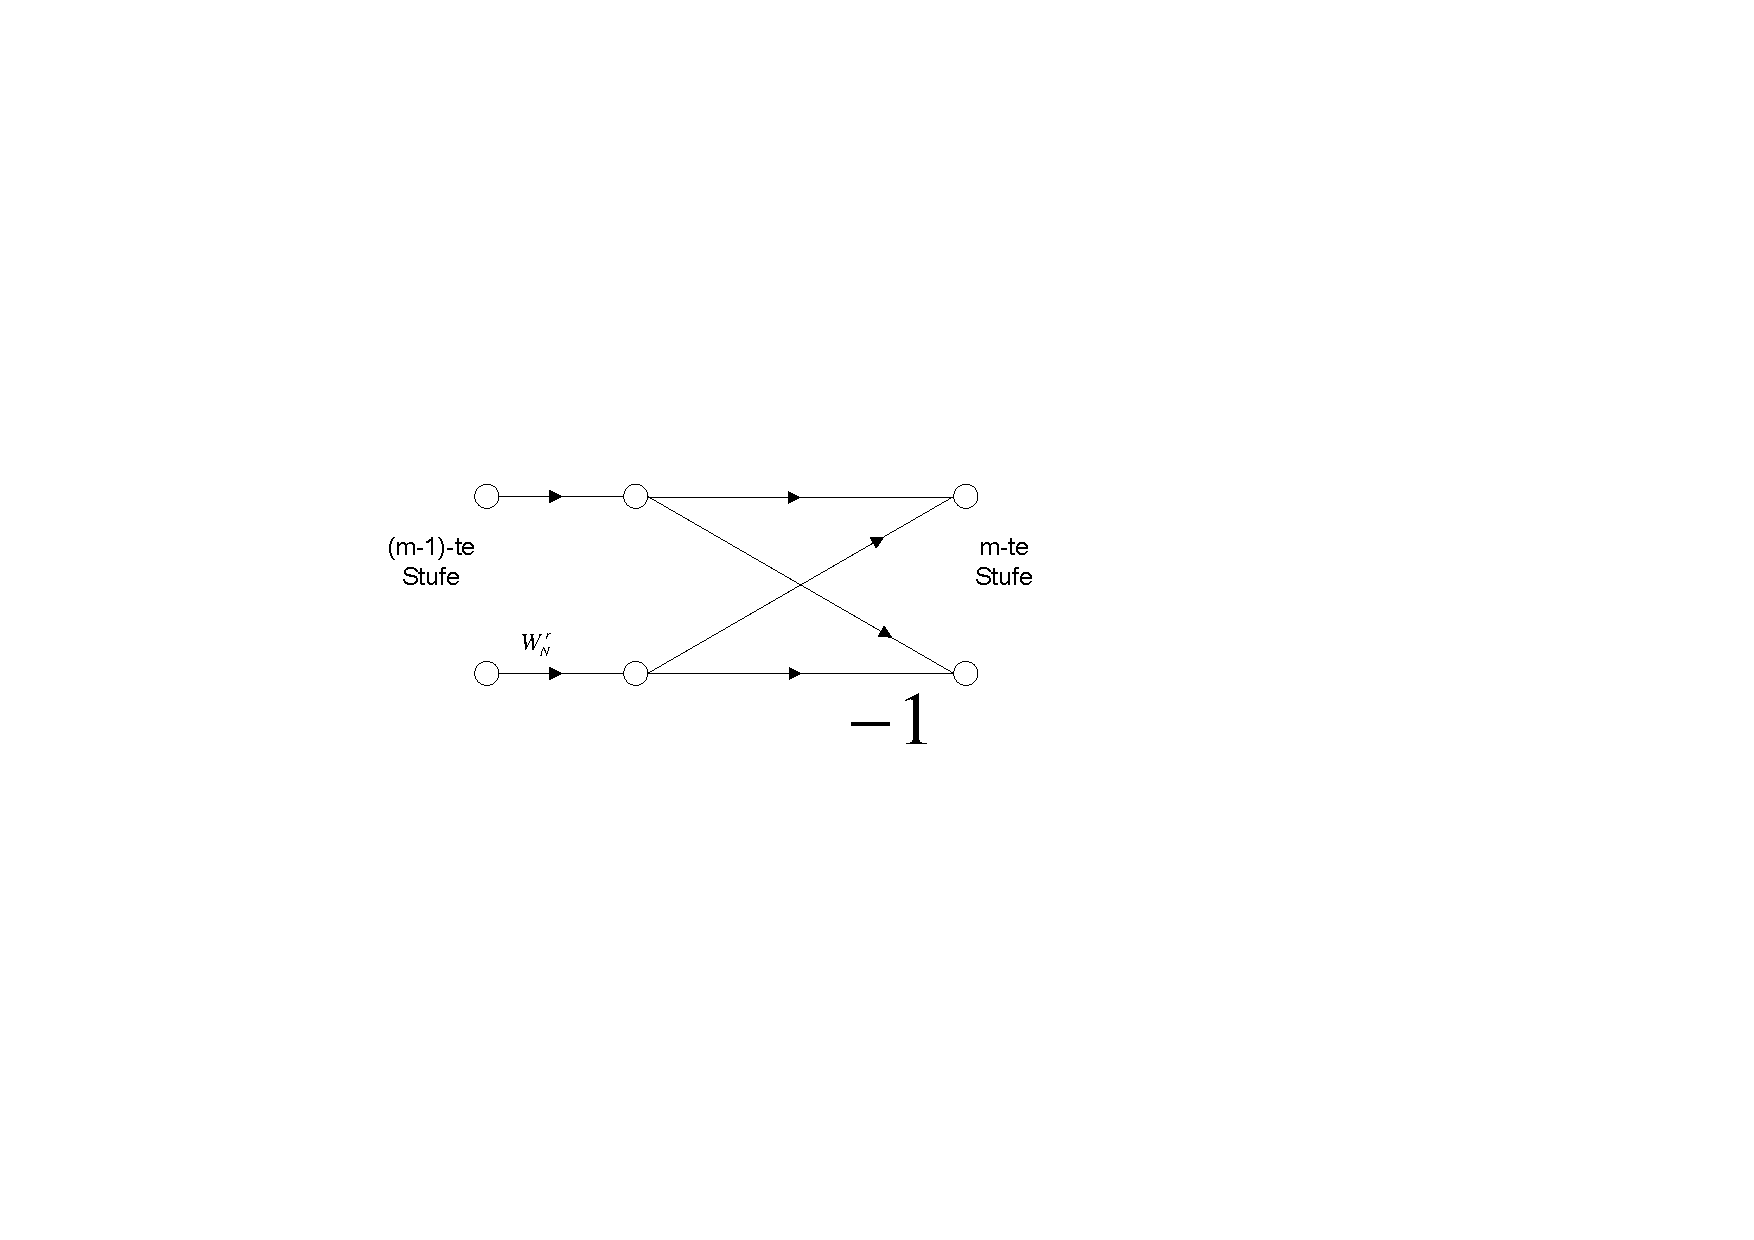
\includegraphics{../Pictures/BF-DIT.pdf}
	\caption{Signalflussgraph eines vereinfachten Butterfly einer DIT\cite{Opp1999}}
	\label{fig:BF-DIT}
\end{figure}
%
Aufgrund der Form dieses Signalflussgraphen wird die dargestellte Operation als \textit{Butterfly} bezeichnet. Der vollst�ndige Signalflussgraph einer 8-Punkte DFT mit Zeitzerlegung ist in \textbf{Abbildung \ref{fig:dit}} zu sehen\cite{Opp1999}.\\
%
\begin{figure}[ht]
	\centering
		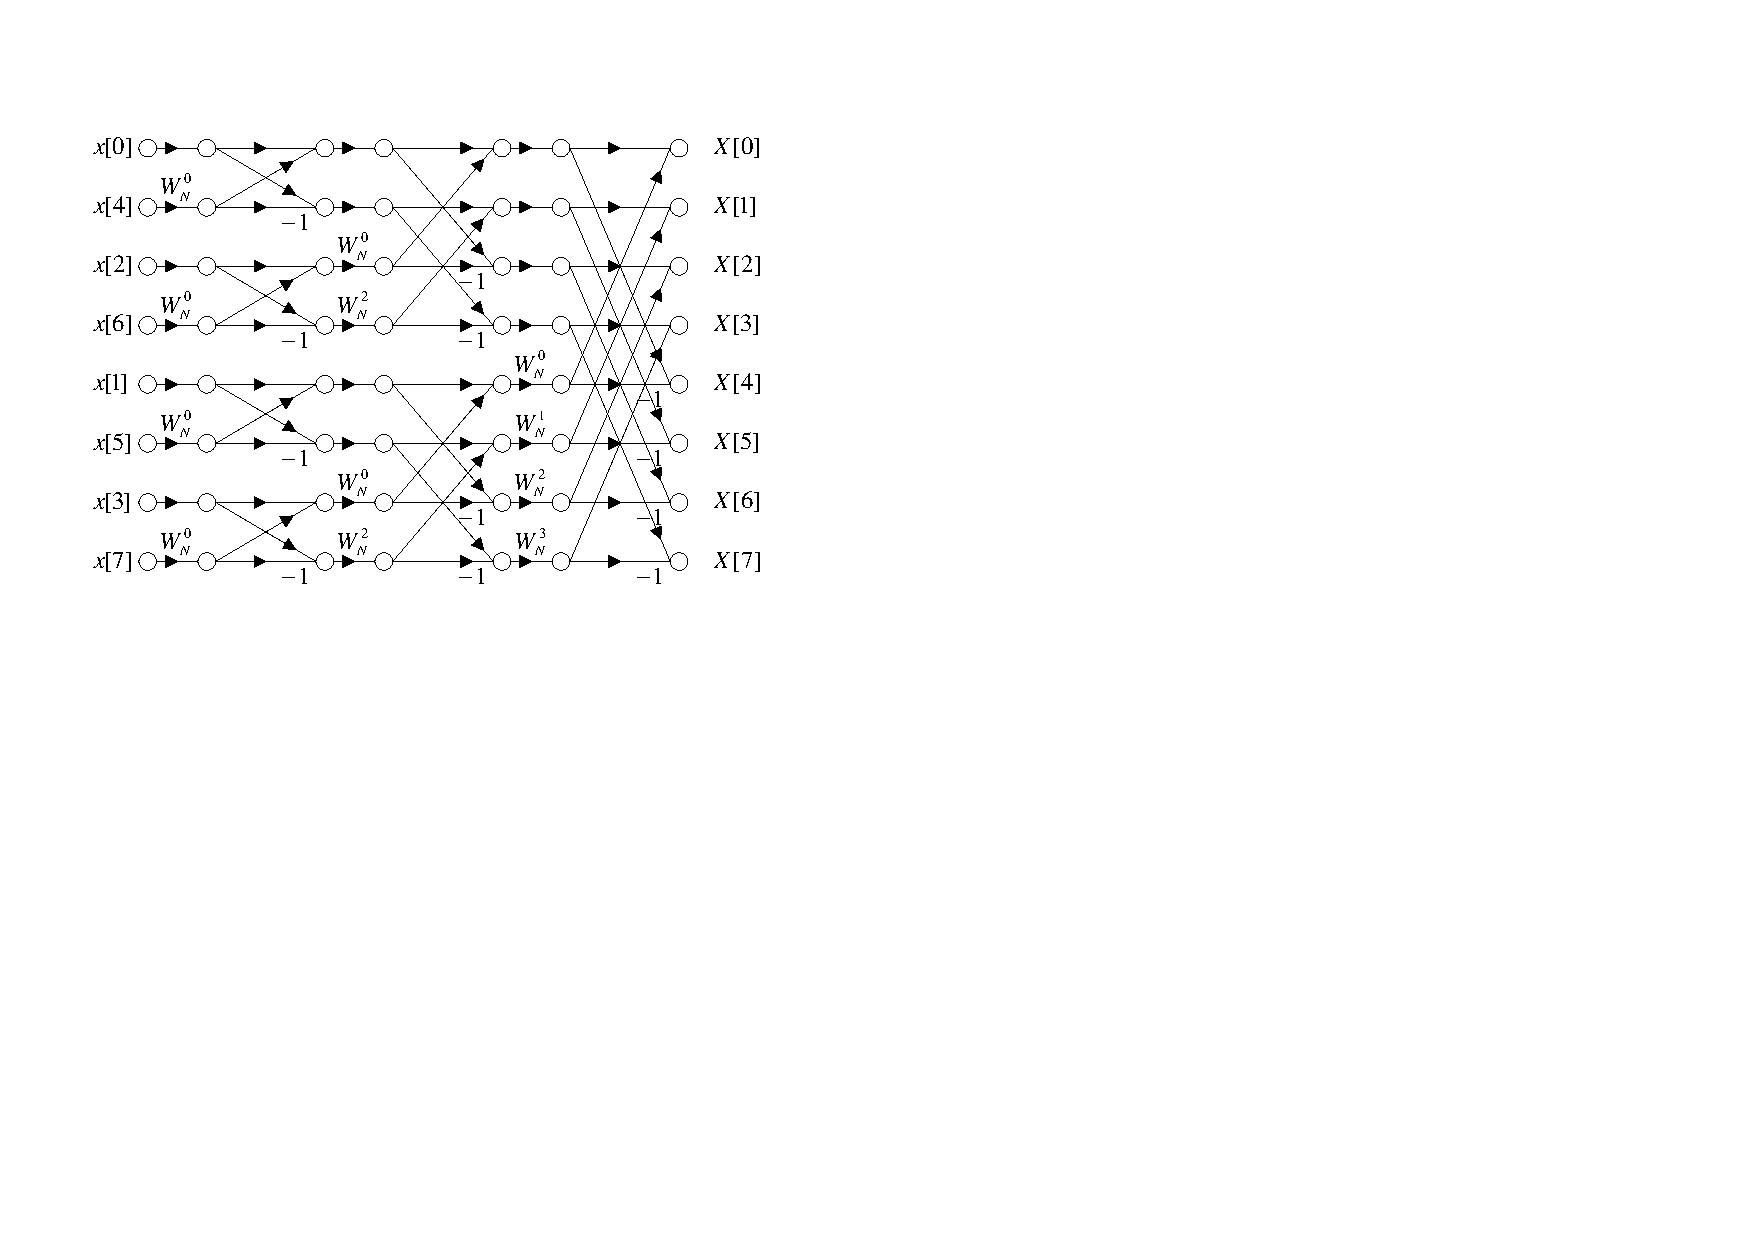
\includegraphics{../Pictures/DIT.pdf}
	\caption{Signalflussgraph einer 8-Punkte DFT mit Zeitzerlegung\cite{Opp1999}}
	\label{fig:dit}
\end{figure}
%
\paragraph{FFT mit Frequenzzerlegung (DIF)}\label{ph:dif}$\;$ \\

Alternativ zur Zeitzerlegung einer FFT kann auch eine Zerlegung der Ausgangsfolge $X[k]$ durchgef�hrt werden, welche als Frequenzzerlegung bezeichnet wird. Hierbei werden wie in \textbf{(\ref{ph:dit})} im ersten Schritt aus der Folge $X[k]$ (\textbf{Formel \ref{eqn:dif1}}) Teilfolgen mit geraden und ungeraden Indizes gebildet (\textbf{Formel \ref{eqn:dif2}}).

\begin{equation}
	\label{eqn:dif1}
	X[k]~=~\sum^{N-1}_{n=0}x[n]W^{nk}_N, ~k=0,1,...,N-1	
\end{equation}

\begin{equation}
	\label{eqn:dif2}
	\begin{split}
	X[2r]~=~\sum^{N-1}_{n=0}x[n]W^{n(2r)}_N, ~r=0,1,...,\frac{N}{2}-1	\\
	X[2r+1]~=~\sum^{N-1}_{n=0}x[n]W^{n(2r+1)}_N, ~r=0,1,...,\frac{N}{2}-1	
	\end{split}
\end{equation}

Diese beiden Folgen k�nnen auch in der in \textbf{Formel \ref{eqn:dif3}} dargestellten Form geschrieben werden.

\begin{subequations}
	\label{eqn:dif3}
	\begin{align}
		X[2r]~=~\sum^{(N/2)-1}_{n=0}x[n]W^{2nr}_N~+~\sum^{N-1}_{n=N/2}x[n]W^{2nr}_N\label{eqn:dif3a}\\
		X[2r+1]~=~\sum^{(N/2)-1}_{n=0}x[n]W^{n(2r+1)}_N~+~\sum^{N-1}_{n=N/2}x[n]W^{n(2r+1)}_N\label{eqn:dif3b}
 	\end{align}
\end{subequations}

F�hrt man an den zweiten Summen der \textbf{Formel \ref{eqn:dif3}} eine Variablensubstitution durch so er gibt sich f�r (\textbf{\ref{eqn:dif3a}}):

\begin{equation}
	\label{eqn:dif4}
	X[2r]~=~\sum^{(N/2)-1}_{n=0}x[n]W^{2nr}_N~+~\sum^{(N/2)-1}_{n=0}x[n+(N/2)]W^{2r(n+(N/2)}_N
\end{equation}

Und f�r die zweite Summe aus (\textbf{\ref{eqn:dif3b}}):

\begin{equation}
	\label{eqn:dif5}
	\begin{split}
		\sum^{N-1}_{n=N/2}x[n]W^{n(2r+1)}_N ~=~ \sum^{(N/2)-1}_{n=0}x[n+(N/2)]W^{[n+(n/2)](2r+1)}_N \\
		=~W^{(N/2)(2r+1)}_N \sum^{(n/2)-1}_{n=0}x[n+(N/2)]W^{n(2r+1)}_N \\
		=~-\sum^{(N/2)-1}_{n=0}x[n+(N/2)]W^{n(2r+1)}_N 
	\end{split}
\end{equation}

Die letzte Umformung aus \textbf{Formel \ref{eqn:dif5}} verwendet die Tatsache, dass $W^{(N/2)2r}_N=1$ und $W^{(N/2)}_N=0$ gilt.\\
Fasst man nun jeweils die Summationen der beiden Teilfolgen zusammen und nutzt wie in (\textbf{\ref{ph:dit}})$W^2_N=W_{N/2}$, kann man die Teilfolgen auch wie in \textbf{Formel \ref{eqn:dif6}} darstellen.

\begin{equation}
	\label{eqn:dif6}
	\begin{split}
		X[2r]~=~\sum^{(N/2)-1}_{n=0}(x[n]+x[n+(N/2)])W^{rn}_{N/2}, ~r=0,1,...,\frac{N}{2}-1 \\
		X[2r+1]~=~\sum^{(N/2)-1}_{n=0}(x[n]+x[n+(N/2)])W^{rn}_{N/2}W^n_N, ~r=0,1,...,\frac{N}{2}-1
	\end{split}
\end{equation}

In \textbf{Abbildung \ref{fig:BF-DIF}} ist der aus \textbf{Formel \ref{eqn:dif6}} abgeleitete Signalflussgraph der \textit{Butterfly}-Operation zu sehen und \textbf{Abbildung \ref{fig:dif}} zeigt den vollst�ndigen Signalflussgraph einer 8-Punkte DFT nach Frequenzzerlegung\cite{Opp1999}.\\
%
\begin{figure}[ht]
	\centering
		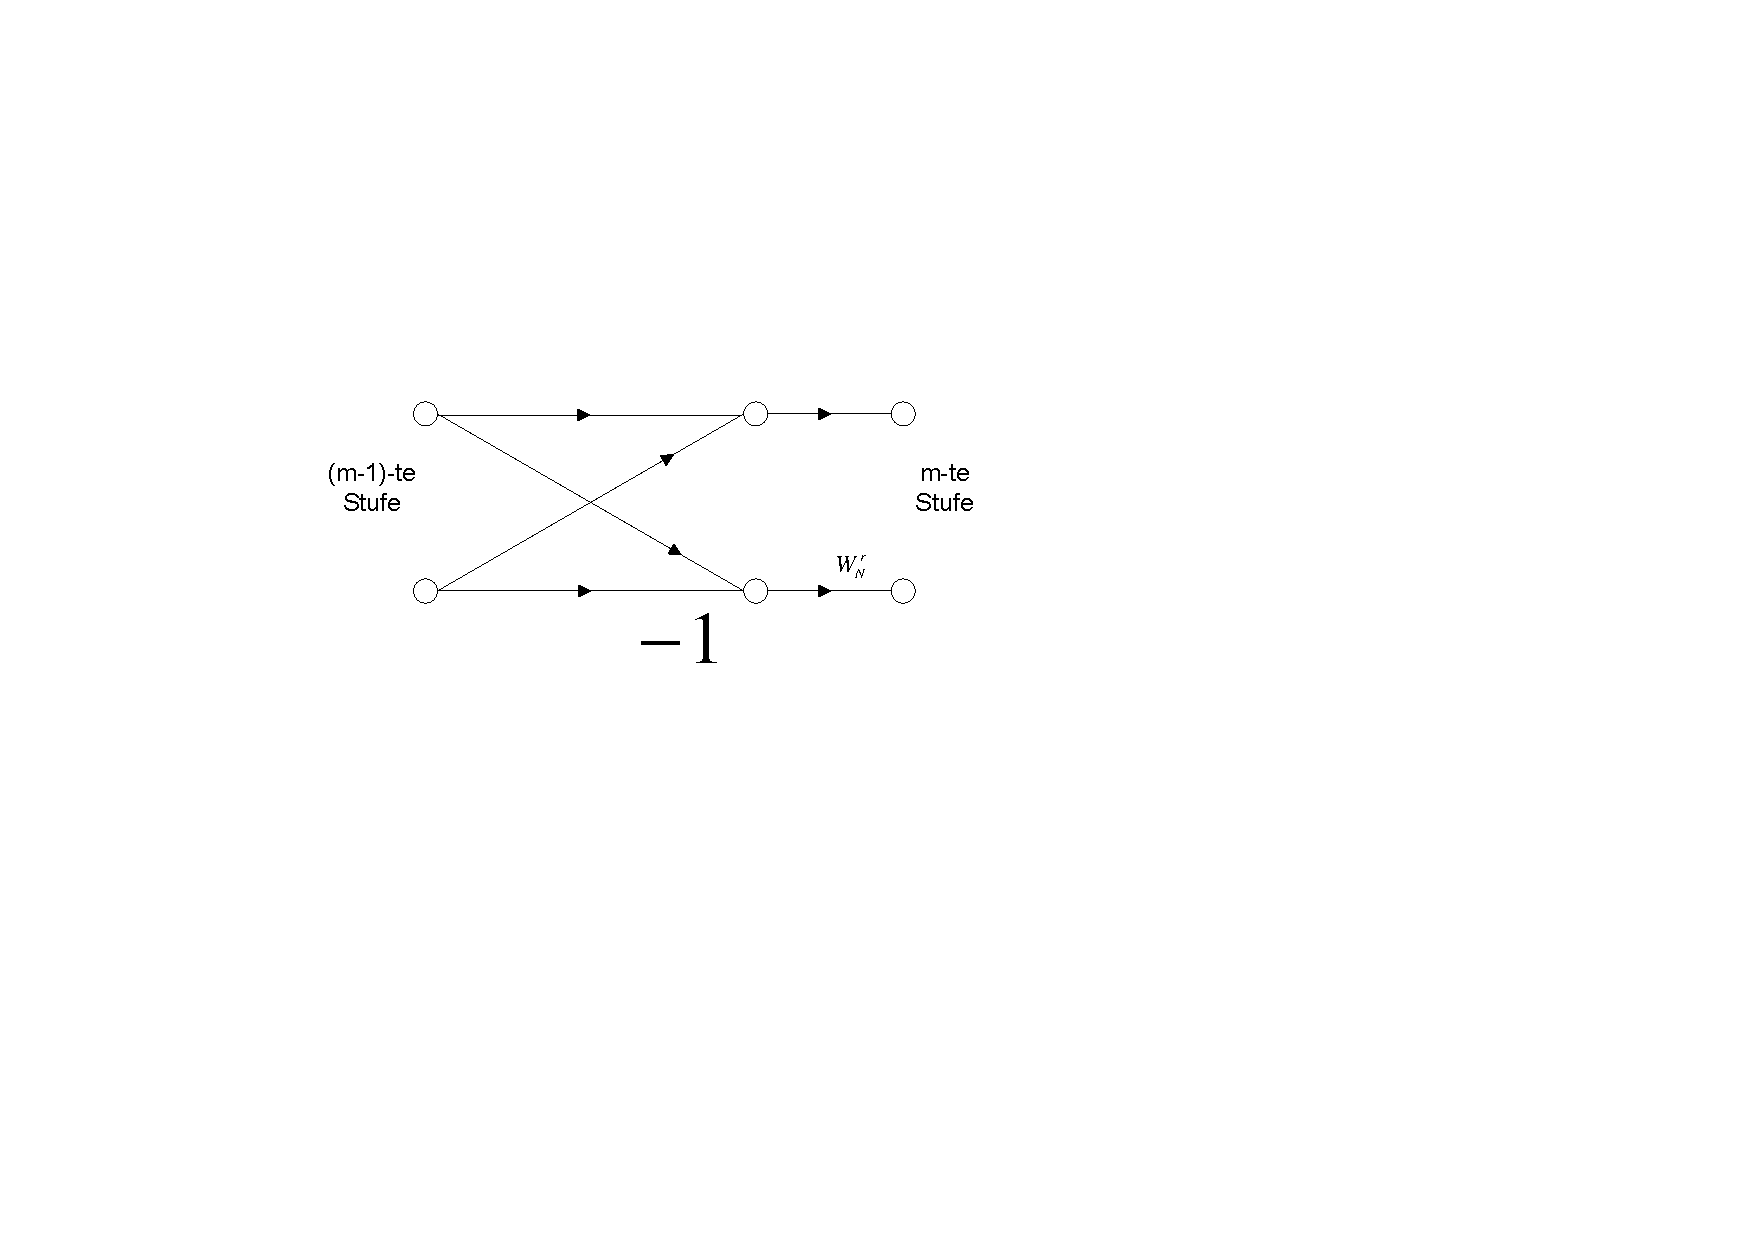
\includegraphics{../Pictures/BF-DIF.pdf}
	\caption{Signalflussgraph eines vereinfachten Butterfly einer DIF\cite{Opp1999}}
	\label{fig:BF-DIF}
\end{figure}
%
\begin{figure}[ht]
	\centering
		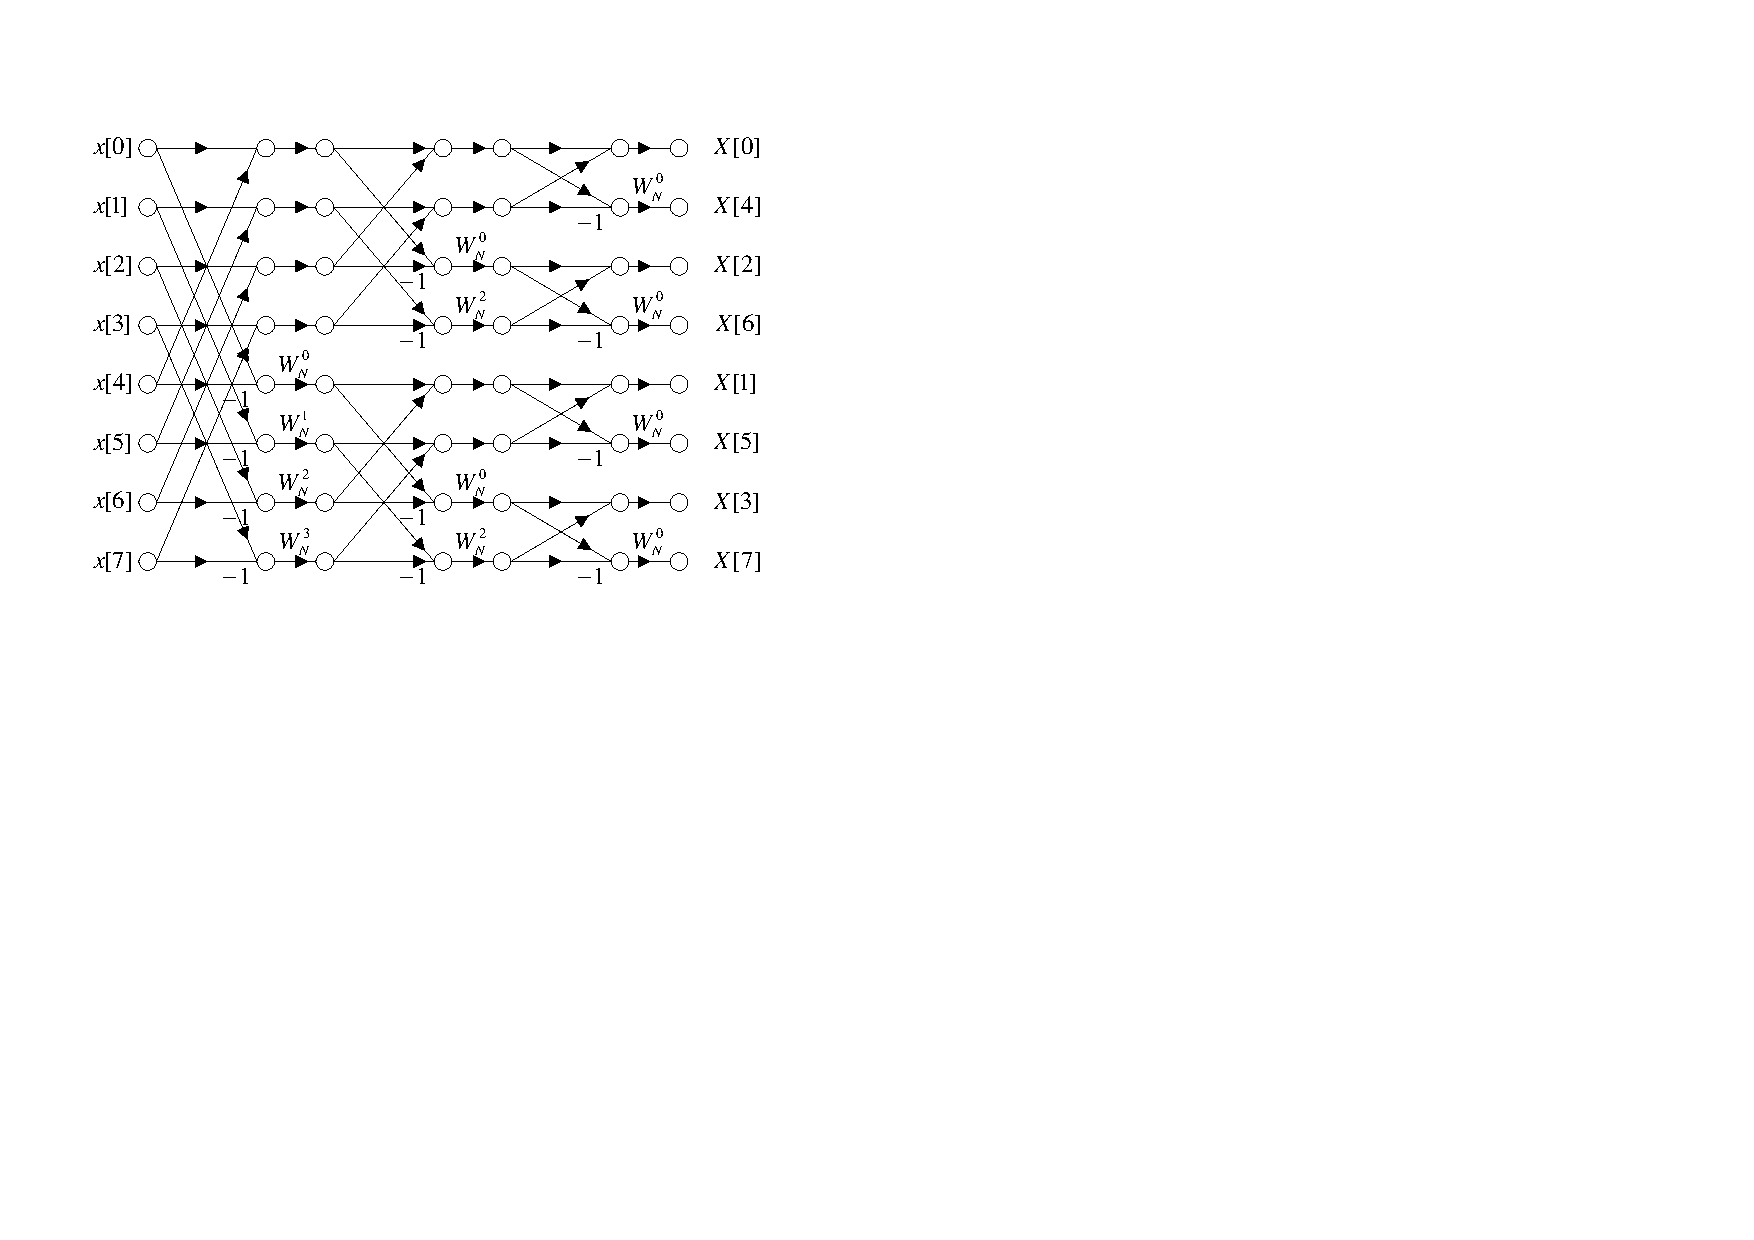
\includegraphics{../Pictures/DIF.pdf}
	\caption{Signalflussgraph einer 8-Punkte DFT mit Frequenzzerlegung\cite{Opp1999}}
	\label{fig:dif}
\end{figure}
%
\paragraph{Bitumkehrungordnung (bit-reversed order)}\label{ph:bit}$\;$ \\

Wie man in \textbf{Abbildung \ref{fig:dit}} und \textbf{Abbildung \ref{fig:dif}} gut erkennen kann, liegen entweder die Eing�nge oder die Ausg�nge in einer nicht numerisch sortierten Form vor. Diese Sortierung ergibt sich aus den in (\textbf{\ref{ph:dit}}) und (\textbf{\ref{ph:dif}}) gezeigten Algorithmen, diese folgt aber immer dem selben Schema.\\ 
Es werden die Indizes des Ein- oder Ausgangs anhand ihrer Bits vom \textit{Least Significant Bit (LSB)} zum \textit{Most Significant Bit (MSB)} sortiert, so dass pro Ebene in der oberen H�lfte die Indizes stehen, die beim momentan betrachteten Bit eine 0 aufweisen.\\
Dieses Prinzip soll in \textbf{Tabelle \ref{tab:bit}} f�r 8-Bit lange Indizes veranschaulicht werden.\\
%
\begin{table}[ht]
	\centering
		\begin{tabular}{c | c | c | c}
			Position (dezimal) & Position (bin�r) & "`bit reversal"' (bin�r) & "`bit reversal"' (dezimal) \\
			\hline\hline
			0 & 000 & 000 & 0\\
			1 & 001 & 100 & 4\\
			2 & 010 & 010 & 2\\
			3 & 011 & 110 & 6\\
			4 & 100 & 001 & 1\\
			5 & 101 & 101 & 5\\
			6 & 110 & 011 & 3\\
			7 &	111 &	111 &	7
		\end{tabular}
	\caption{Bitumkehrordnung f�r 8-Bit Indizes\cite{haller2008}}
	\label{tab:bit}
\end{table}
%
\subsubsection{Amplitude of Spectrum}\label{subsubsec:aos}
Bei der Amplitude of Spectrum wird werden die normalisierten Spektralkomponenten eines Fenster berechnet. \\
Hierf�r wird zu erst der Betrag der diskreten Transformierten berechnet, der danach durch die Gr��e des betrachteten Fensters geteilt wird (\textbf{Formel \ref{eqn:aos}}).

\begin{equation}
	\label{eqn:aos}			   
	A(k)~=~\frac{\sqrt{\Re\left[X(k)\right]^2+\Im\left[X(k)\right]^2}}{N}
\end{equation}

\subsubsection{Chroma Vektor}\label{subsubsec:cv}

Der Chroma Vektor fasst alle Spektralkomponenten einer Tonh�he zusammen und fasst alle Frequenzen zu einer Oktave zusammen. Hierbei werden alle spektralen Amplituden des gleichen Halb- oder Vierteltons aufsummiert (\textbf{Formel \ref{eqn:cv}}).

\begin{equation}
	\label{eqn:cv}			   
	A_{chroma}\left(\widetilde{k}\right)~=~\sum_{k:~p(k)=\widetilde{k}} A(k)
\end{equation}

Z.B. f�r Viertelt�ne gilt

\[p(k)~=~\left\lfloor 24~log_{2}\left(\frac{2k}{N}\frac{f_{s}}{f_{1}}\right) \right\rfloor~mod~24\textrm{ und }f_{1}~=~440~Hz \]

F�r Halbt�ne m�sste 24 durch 12 ersetzt werden\cite{haller2008}\cite{Theimer2008}.

\subsubsection{Amplitude Of Maximum In Chromagram}\label{subsubsec:aomic}

Die maximale Amplitude des Chromagrams gibt den maximalen Chroma Vektor an und stellt daher die St�rke eines Tons in verschiedenen Oktavstufen dar (\textbf{Formel \ref{eqn:aomic}})\cite{haller2008}\cite{Theimer2008}.

\begin{equation}
	\label{eqn:aomic}			   
	A_{maxchroma}~=~\max_{\widetilde{k}}~A_{chroma}\left(\widetilde{k}\right)
\end{equation}

\subsubsection{Mel Frequency Cepstral Coefficients (MFCC)}\label{subsubsec:mfcc}

Das Cepstrum ist definiert als die Fouriertransformation (oder die DCT) des logerithmierten Amplitudenspektrums.\\
Normalerweise wird ein Cepstrum auf der Basis des Frequenzspektrums berechnet, f�r die Berechnung der MFCC wird allerdings das Mel-Band zugrunde gelegt. Das Mel-Band basiert auf der Mel-Skala, die als psychoakustische Ma�einheit definiert ist. Wird zum Beispiel eine Frequenz als doppelt so hoch wahrgenommen wie eine festgelegte Referenzfrequenz, so wird auf der Mel-Skala diesem auch der doppelte Wert dieser Referenzfrequenz zugewiesen. Die hierf�r verwendete Referenzfrequenz liegt bei 1000 Hz.\\
Soll nun eine Frequenz $f$ in den zugeh�rigen Mel-Wert $m$ umrechnen werden, wird hierf�r die \textbf{Formel \ref{eqn:mel}} verwendet.

\begin{equation}
	\label{eqn:mel}			   
	m~=~2595 \log_{10} \left(1+\frac{f}{700}\right)
\end{equation}

F�r die Berechnung der MFCC wird in 4 Schritten durchgef�hrt.\\
Als Erstes wird wie bei allen Features des Frequenzbereiches die Spektralkomponenten durch eine Fouriertransformation berechnet. Der zweite Schritt besteht in einer Bandpassfilterung dieser Spektralkomponenten nach \textbf{Formel \ref{eqn:melm}}.

\begin{equation}
	\label{eqn:melm}			   
	M(k')~=~\sum\limits^{\frac{K}{2}-1}_{k=0}A(k)\cdots w_{k'}(k)
\end{equation}

Hierbei beschreibt $w_{k'}(k)$ Dreiecksfenster, deren Breite f�r wachsendes $k$ zunehmen. Im Normalfall wird f�r diese Transformation in das Mel-Band 12 oder 24 Dreiecksfenster verwendet, wobei die Anzahl der Dreiecksfenster gleichzeitig die Aufl�sung der Transformation beschreibt.\\
Im n�chsten Schritt wird der Logarithmus von $M(k')$ gebildet. Letztendlich wird zur Berechnung der MFCC eine Diskrete Cosinuns Transformation (DCT) durchgef�hrt.\\
Wird die Bandpassfilterung mit 12 Dreiecksfenstern durchgef�hrt, liefert dieser Algorithmus einen Ergebnisvektor mit 13 Komponenten \cite{Lee2009}\cite{haller2008}\cite{Theimer2008}. 

\subsubsection{Normalized Audio Spectrum Envelope}\label{subsubsec:nase}

Der Normalized Audio Spectrum Envelope (NASE) gibt Auskunft �ber das Energiespektrum jedes Fensters. Hierbei wird pro Fenster ein Vektor generiert, bei dem jedes Vektorelement die normalisierte, quadrierte Magnitude eines definierten Frequenz-Unterbandes entspricht.\\
Die Frequenz-Unterb�nder spannen sich logarithmisch zwischen 62.4 Hz ("`loEdge"') und 16 kHz ("`hiEdge"') �ber 8 Oktaven. Die Anzahl $B$ von Unterb�ndern wird hierbei mit

\begin{equation}
	\label{eqn:naseb}			   
	B~=~\frac{8}{r}
\end{equation}
berechnet, wobei $r$ f�r die Spektralaufl�sung steht und 

\begin{equation}
	\label{eqn:naser}			   
	r~=~2^j Oktaven,~-4\leq j \leq 3
\end{equation}
gilt (vgl. \textbf{Abbildung \ref{fig:nase}}).

\begin{figure}[htbp]
	\centering
		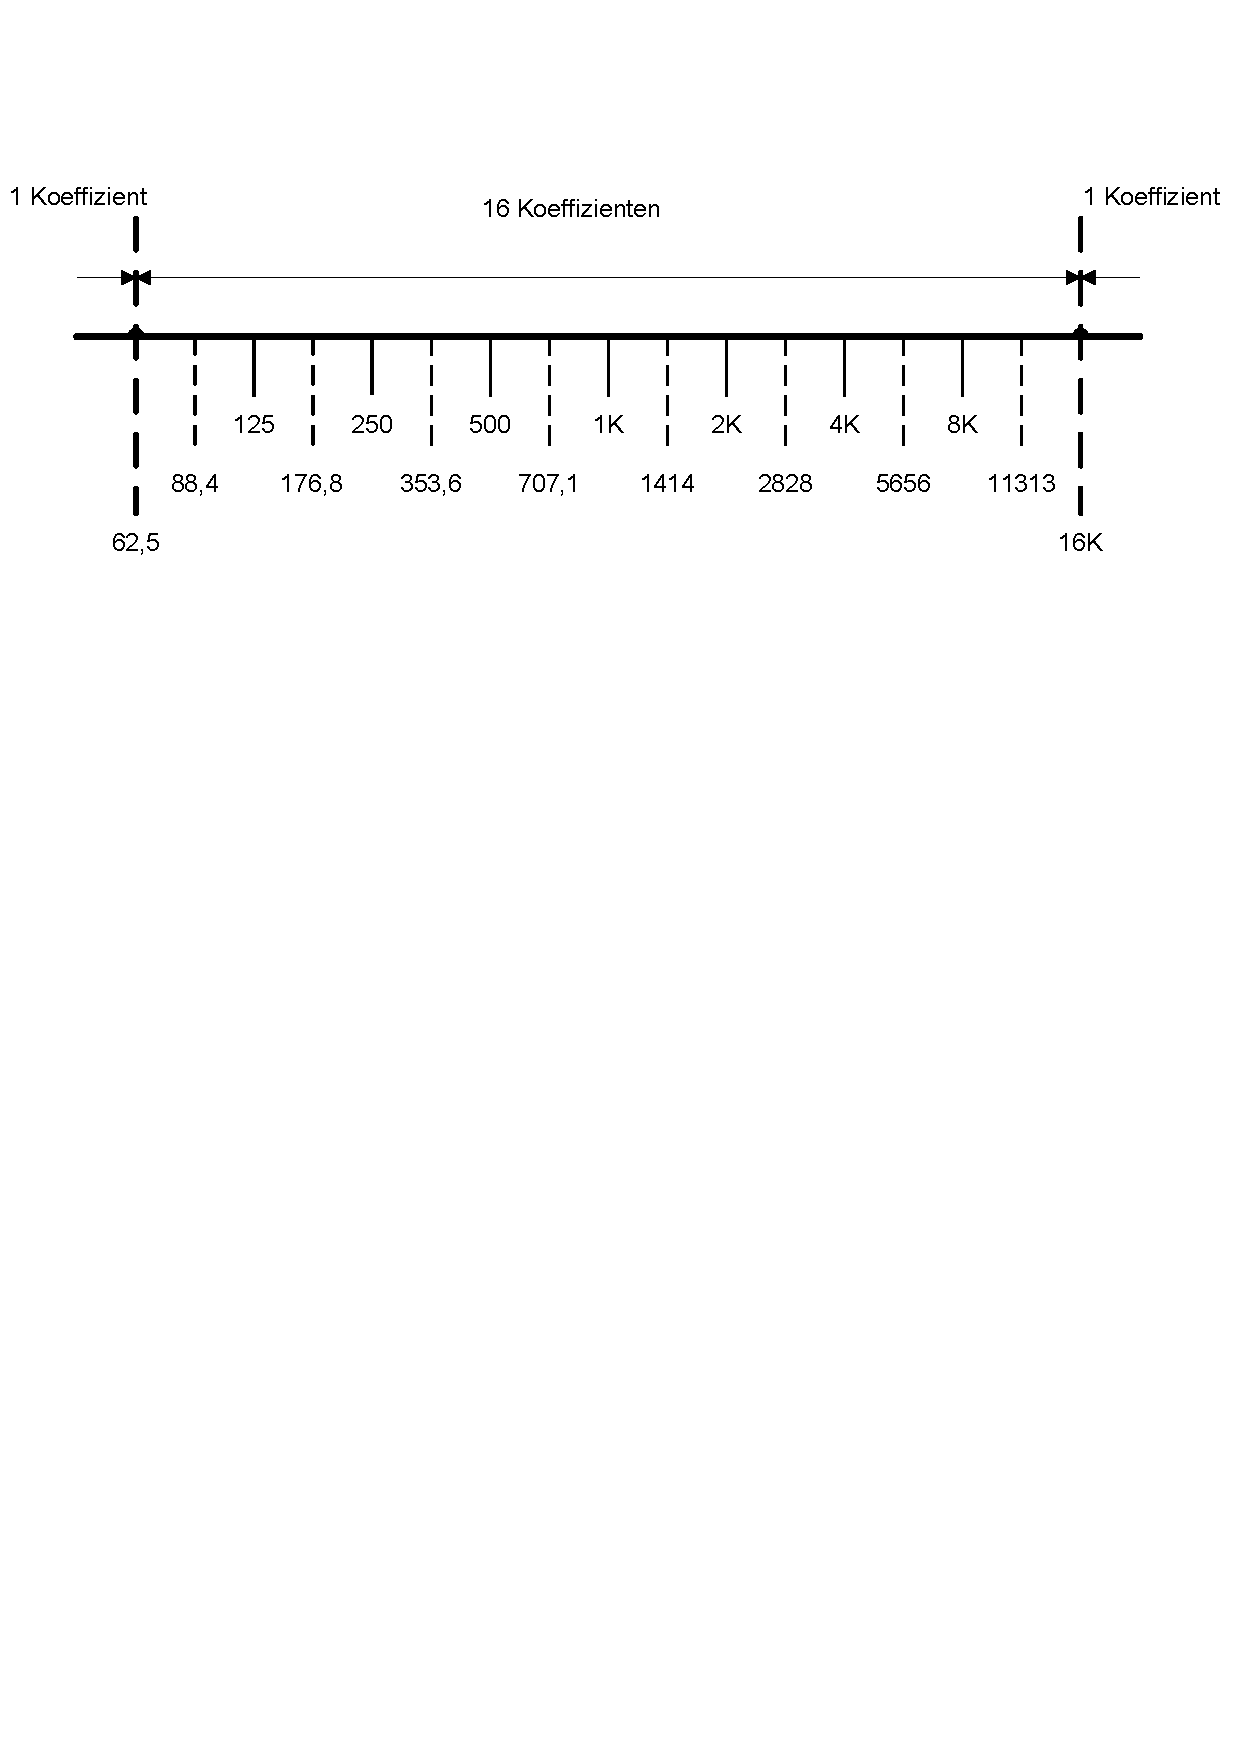
\includegraphics[width=1.00\textwidth]{../Pictures/NASE-coeff.pdf}
	\caption{NASE Unterb�nder f�r eine spektrale Aufl�sung von $\frac{1}{2}$ \cite{Lee2009}}
	\label{fig:nase}
\end{figure}

Die Berechnung der einzelnen NASE-Werte erfolgt hierbei in drei Schritten.\\
Als erstes wird f�r jedes Unterband $b$ der Audio Spectral Envelope (ASE) nach der in \textbf{Formel \ref{eqn:ase}} gegebenen Formel berechnet.

\begin{equation}
	\label{eqn:ase}			   
	ASE(b)~=~\sum^{hiKb}_{k=loKb}P(k),~0\leq b \leq B+1
\end{equation}

Danach werden diese ASE-Werte nach \textbf{Formel \ref{eqn:asedb}} in Dezibelwerte umgerechnet.

\begin{equation}
	\label{eqn:asedb}			   
	ASE_{dB}(b)~=~10\log_{10}(1+ASE(b)),~0 \leq b \leq B+1
\end{equation}

Anschlie�end wird aus diesen Werten der NASE-Wert f�r die einzelnen Unterb�nder $b$ berechnet (\textbf{Formel \ref{eqn:nase}}).

\begin{equation}
	\label{eqn:nase}			   
	NASE(b)~=~\frac{ASE_{dB}(b)}{R},~0\leq b \leq B+1
\end{equation}

Hierbei steht $R$ f�r den normierten RMS-Wert, der nach \textbf{Formel \ref{eqn:naserms}} berechnet wird.

\begin{equation}
	\label{eqn:naserms}			   
	R~=~\sqrt{\sum^{B+1}_{b=0}\left(ASE_{dB}(b)\right)^2}
\end{equation}

Aus den einzelnen NASE-Werten der einzelnen Unterb�nder wird abschlie�end der Ergebnisvektor $X_{NASE}$ gebildet (\textbf{Formel \ref{eqn:nasex}})\cite{Lee2009}.

\begin{equation}
	\label{eqn:nasex}			   
	x_{NASE}~=~\left[R,NASE(0),NASE(1),...,NASE(B+1)\right]^T
\end{equation}

\subsubsection{Octave Spectral Contrast}\label{subsubsec:osc}

Beim Octave Spectral Contrast wird das Frequenzspektrum als erstes via Bandpass-Filtern in Unterb�nder aufgeteilt (siehe \textbf{Tabelle \ref{tab:osc}}), danach werden f�r jedes Unterband \textit{spektrale Peaks} (\textbf{Formel \ref{eqn:peak}}) und\textit{spektrale Valleys}(\textbf{Formel \ref{eqn:valley}}) berechnet, wobei Peaks den harmonischen Komponenten und Valleys nicht-harmonischen Komponenten oder Rauschen des Unterbandes $b$ entsprechen. Hierbei werden die Power Spektren $P_{b,n}$ vorher so sortiert, dass $P_{b,1}\geq P_{b,2}\geq ... \geq P_{b,n}$ gilt.\\
\begin{table}[ht]
	\centering
		\begin{tabular}{c | c}
			Filternummer & Frequenzbereich (Hz)\\
			\hline\hline
			0 & [0,0]\\
			1 & (0,100]\\
			2 & (100, 200]\\
			3 & (200, 400]\\
			4 & (400, 800]\\
			5 & (800, 1600]\\
			6 & (1600, 3200]\\
			7 & (3200, 6400]\\
			8 & (6400, 12800]\\
			9 & (12800, 22050]\\
			
		\end{tabular}
	\caption{Frequenzbereiche der Bandpass-Filter bei 44.1 kHz Samplingfrequenz\cite{Lee2009}}
	\label{tab:osc}
\end{table}
%
\begin{equation}
	\label{eqn:peak}			   	
	Peak(b)~=~\log\left(\frac{1}{\alpha N_b}\sum\limits^{\alpha N_b}_{i=1}P_{b,i}\right)
\end{equation}
\begin{equation}
	\label{eqn:valley}			   	
	Valley(b)~=~\log\left(\frac{1}{\alpha N_b}\sum\limits^{\alpha N_b}_{i=1}P_{b,N_b - i+1}\right)
\end{equation}
Hierbei ist $\alpha$ ein Nachbarschaftsfactor, der in der Literatur mit 0,2 angenommen wird. Der spektrale Kontrast eines Unterbandes errechnet sich nun als Differenz von $Peak(b)$ und $Valley(b)$ (\textbf{Formel \ref{eqn:oscsc}}).
\begin{equation}
	\label{eqn:oscsc}			   	
	SC(b)~=~Peak(b)~-~Valley(b)
\end{equation}
Und der resultierende Featurevektor $x_{OSC}$ abschlie�end aus den Valleys und spektralen Kontrasten eines Audioframes (\textbf{Formel \ref{eqn:osc}})\cite{Lee2009}.

\begin{equation}
	\label{eqn:osc}			   	
	x_{OSC} = \left[Valley(0=,...,Valley(B-1),SC(0),...SC(B-1)\right]^T
\end{equation}

%\subsubsection{Power Spectrum}\label{subsubsec:ps}
%
%Das Power Spectrum berechnet sich indem man den Logarithmus des Amplitudenspektrums berechnet (\textbf{Formel \ref{eqn:ps}})\cite{haller2008}.
%
%\begin{equation}
%	\label{eqn:ps}			   	
%	S(k)~=~10\cdot\log\limits_{10}\left(\frac{1}{N}A^2(k)\right)
%\end{equation}



\subsubsection{Spectral Centroid}\label{subsubsec:sc}

Der Spectral Centroid gibt den Schwerpunkt des Amplitudenspektrums des Signals an (\textbf{Formel \ref{eqn:sc}})\cite{haller2008}\cite{Theimer2008}.

\begin{equation}
	\label{eqn:sc}			   	S_{centroid}~=~\frac{\sum\limits^{\frac{K}{2}-1}_{k=0}k~A(k)}{\sum\limits^{\frac{K}{2}-1}_{k=0}A(k)} 
\end{equation}

\subsubsection{Spectral Crest Factor}\label{subsubsec:scf}

Der Spectral Crest Factor stellt ein Ma� der spektralen Flachheit eines Frequenzbandes dar und ist im Wertebereich $\left[1,\infty\right]$ definiert. Hierbei bedeutet 1, dass alle spektral Amplituden gleich sind und $\infty$ das gar keine Flachheit existiert (\textbf{Formel \ref{eqn:scf}}).\\
Dieser Faktor wird auf folgenden Frequenzb�ndern berechnet\cite{Theimer2008}:
\begin{itemize}
	\item 250 - 500 Hz ($k_{1l}$ - $K_{1u}$)
	\item 500 - 1000 Hz ($k_{2l}$ - $K_{2u}$)
	\item 1000 - 2000 Hz ($k_{3l}$ - $K_{3u}$)
	\item 2000 - 4000 Hz ($k_{4l}$ - $K_{4u}$)
\end{itemize}


\begin{equation}
	\label{eqn:scf}			   
	S_{crest}~=~frac{\max\limits_{k\in\left[k_{il},k_{iu}\right]}A(k)}{\frac{1}{k_{iu}~-~k_{il}~+~1}\sum\limits^{k_{iu}}_{k=k_{il}}A(k)}
\end{equation}

\subsubsection{Spectral Flux}\label{subsubsec:sf}

Der Spectral Flux ist definiert als die quadrierte Differenz zwischen den normalisierten Betragsspektren von zwei aufeinander folgenden Zeitfenstern (\textbf{Formel \ref{eqn:sf}})\cite{haller2008}\cite{Theimer2008}.

\begin{equation}
	\label{eqn:sf}			   
	S_{flux}~=~\frac{2}{K}\sum\limits^{\frac{K}{2}-1}_{k=0}\left( A^{(l)}(k)~-~A^{(l-1)}(k)\right)^2
\end{equation}


\subsubsection{Spectral Rolloff}\label{subsubsec:sr}

Als Spectral Rolloff bezeichnet man der Frequenzwert ($k_{rolloff}$) unter dem sich eine bestimmte Prozentzahl ($p_{rolloff}$) der Spektralwerte konzentrieren (\textbf{Formel \ref{eqn:sr}})\cite{haller2008}\cite{Tza2002}. 

\begin{equation}
	\label{eqn:sr}			   
	\sum^{k_{rolloff}}_{k=0}A(k)~=~p_{rolloff}~\cdot~\sum^{\frac{K}{2}-1}_{k=0}A(k)
\end{equation}

\subsubsection{Sub-Band Energy Ratio}\label{subsubsec:sber}

Die Sub-Band Energy Ratio gibt die Verteilung der Spektralenergie auf die Frequenzintervalle $\left[0,\frac{f_s}{16}\right)$,$\left[\frac{f_s}{16},\frac{f_s}{8}\right)$,$\left[\frac{f_s}{8},\frac{f_s}{4}\right)$ und $\left[\frac{f_s}{4},\frac{f_s}{2}\right)$ an und kann in Indexbereiche $\left[0,\frac{K}{16}\right)$,$\left[\frac{K}{16},\frac{K}{8}\right)$,$\left[\frac{K}{8},\frac{K}{4}\right)$ und $\left[\frac{K}{4},\frac{K}{2}\right)$ �berf�hrt werden (\textbf{Formel \ref{eqn:sber}})\cite{Theimer2008}.

\begin{equation}
	\label{eqn:sber}			   
	S_1~=~\frac{\sum\limits^{\frac{K}{16}-1}_{k=0}A^2(k)}{\sum\limits^{\frac{K}{2}-1}_{k=0}A^2(k)},~S_2~=~\frac{\sum\limits^{\frac{K}{8}-1}_{k=\frac{K}{16}}A^2(k)}{\sum\limits^{\frac{K}{2}-1}_{k=0}A^2(k)},S_3~=~\frac{\sum\limits^{\frac{K}{0}-1}_{k=\frac{K}{8}}A^2(k)}{\sum\limits^{\frac{K}{2}-1}_{k=0}A^2(k)},S_1~=~\frac{\sum\limits^{\frac{K}{2}-1}_{k=\frac{K}{4}}A^2(k)}{\sum\limits^{\frac{K}{2}-1}_{k=0}A^2(k)}
\end{equation}


\section{Profiling}\label{sec:prof}
Der Begriff Profiling beschreibt Methoden, mit denen das Verhalten von Applikationen auf Systemebene analysiert werden k�nnen, hierzu z�hlen Analysen der Laufzeit, der Schreib- und Lesezugriffe und auch die Verh�ltnisse von Instruktionen und Takten zueinander. Im Folgenden werden nun Beispielhaft die Profilingmethoden der Laufzeitmessung, der richtigen Vorhersagen des Vorladens in den Cache (sog. Cache Hits), sowie die Betrachtungen des Verh�ltnisses von Takt und Instruktionen (Instructions per Cycle (IPC) und Cycle per Instruction (CPI)).

\subsection{Laufzeitanalyse}\label{subsec:time}

\subsection{Cache Hits}\label{subsec:cache}

\subsection{IPC und CPI}\label{subsec:ipccpi}


\chapter{Das EVM8168-Entwicklungsboard}
\label{ch:board}
\rm

F�r die in den folgenden Kapiteln beschriebenen Arbeitsschritte zur Optimierung und Analyse des Programmes wurde ein EVM8168-Entwicklungsboard verwendet, welches von der Firma Texas Instruments in Zusammenarbeit mit der Firma Spectrum Digital entwickelt wurde.
Dieses Board kann mit Hilfe eines DM816x (DaVinci\texttrademark) ARM-Prozessors entweder selber Programme ausf�hren oder es k�nnen auch die beiden ARM-Prozessoren C6A816x (Integra\texttrademark) oder AM389x (Sitara\texttrademark) emuliert werden. 


\section{Aufbau des EVM8168} \label{sec:evm816}
Wie in \cite{spec} beschrieben bietet das EVM816x-Entwicklungsboard eine Standalone-Plattform um Programme f�r DaVinci\texttrademark, Integra\texttrademark~oder Sitara\texttrademark~Prozessoren der Firma Texas Instruments zu entwickeln und zu debuggen. Hierf�r sind neben dem DaVinci\texttrademark~noch weitere On-Board Peripherie auf dem Board aufgebracht, die im folgenden aber nicht n�her erl�utert werden sollen.
Das EVM8168-Board hat unter anderem folgende Komponenten integriert:

\begin{itemize}
	\item DM816x- (DaVinci\texttrademark-)ARM Prozessor (\textbf{Kapitel~\ref{sec:davinci}}) mit NEON-Coprozessor (\textbf{Kapitel~\ref{subsubsec:neon}}) und DSP (\textbf{Kapitel~\ref{subsec:dsp}})
	\item 1 GB DDR3-RAM
	\item AC31061-Audiochip
	\item Gigabit Ethernet
	\item HDMI
	\item VGA
	\item USB

\end{itemize}

\textbf{Abbildung~\ref{fig:top_ti816x_evm}} zeigt eine Draufsicht auf das Entwicklungsboard und die unterhalb dessen angebrachte Daughtercard mit weiteren Anschlussm�glichkeiten.

\begin{figure}[htbp]
	\centering
		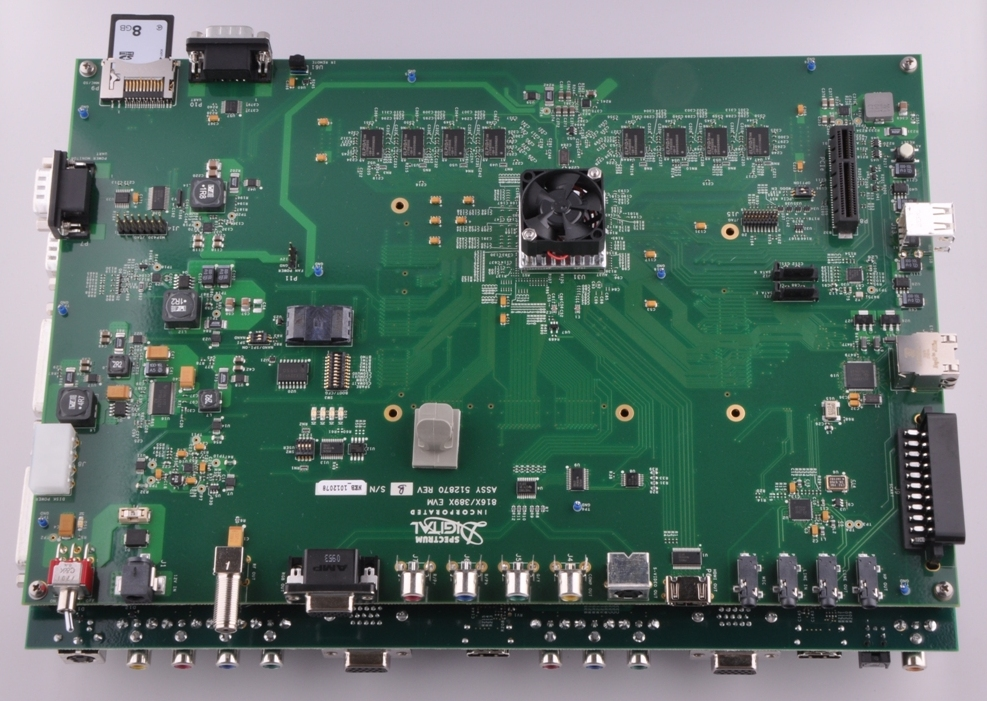
\includegraphics[scale=0.4]{../Pictures/top_ti816x_evm.png}
	\caption{Draufsicht auf das EVM8168}
	\label{fig:top_ti816x_evm}
\end{figure}



\section{Der DaVinci\texttrademark}\label{sec:davinci}
Bei dem auf dem EVM816x verwendeten ARM-Prozessor DM816x handelt es sich um einen eigentlich f�r die Videoprozessierung optimierten Prozessor der DaVinci\texttrademark-Familie von Texas Instruments.\\
Der DM816x ist ein heterogener Prozessor, der mehreren Subsystemen und Coprozessoren besteht.
Genauer gibt des folgende Subsysteme:

\begin{itemize}
\item ARM Subsystem mit einem Cortex-A8 der Firma ARM (\textbf{\ref{subsec:a8}})
\item DSP Subsystem mit einem C674x VLIW DSP der Firma Texas Instruments (\textbf{\ref{subsec:dsp}})
\item SGX530 3D Grafik Engine
\item 512kb On-Chip RAM
\item High-Definition Video Image Coprozessoren (HDVICP2)
\item Media Controller
\item HD Video Processing Subsystem (HDVPSS)
\item System Control
\item Peripherie
\end{itemize} 

All diese Subsysteme und Coprozessoren sind durch eine gemeinsame System Interconnection miteinander verbunden. \textbf{Abbildung \ref{fig:dm8168}} zeigt das funktionale Blockdiagramm des DM816x.\\
%
\begin{figure}[htbp]
	\centering
		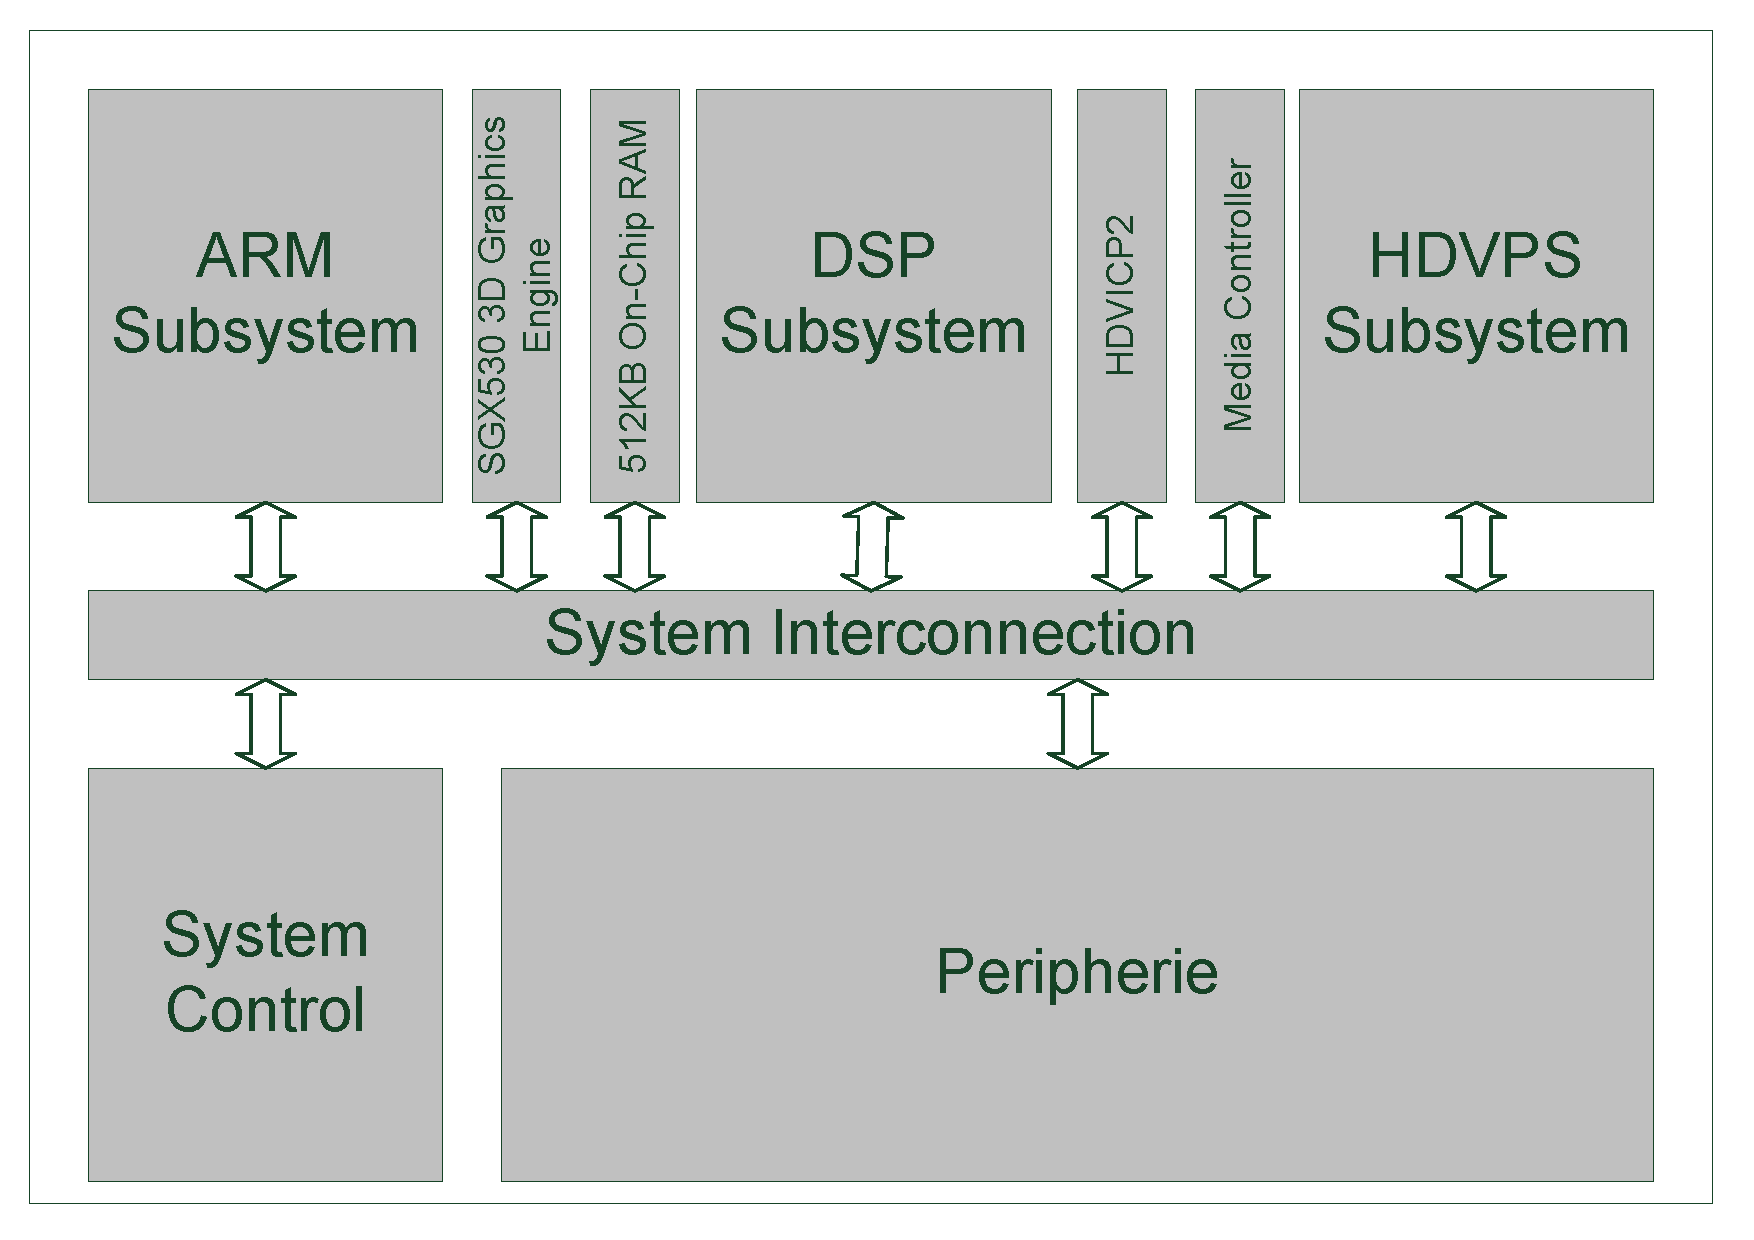
\includegraphics[scale=0.5]{../Pictures/dm8168.pdf}
	\caption{Funktionales Blockdiagramm des DM816x\cite{evm8168}}
	\label{fig:dm8168}
\end{figure}
%

\subsection{ARM Cortex-A8}\label{subsec:a8}

Der erste Prozessor aus der heterogenen Prozessorarchitektur des DM8168 der vorgestellt werden soll, ist ein Cortex-A8 der Firma ARM. Hierbei handelt des sich um einen General-Purpose Prozessor im RISC Design. Er besteht im wesentlichen aus 6 Komponenten (vgl. \textbf{Abbildung \ref{fig:a8}}):

\begin{itemize}
	\item Instruction Fetch
	\item Instruction Decode
	\item Instruction Execute
	\item Load/Store
	\item L2 Cache
	\item NEON-Coprozessor (\textbf{\ref{subsubsec:neon}})
\end{itemize}
%
\begin{figure}[h]
	\centering
		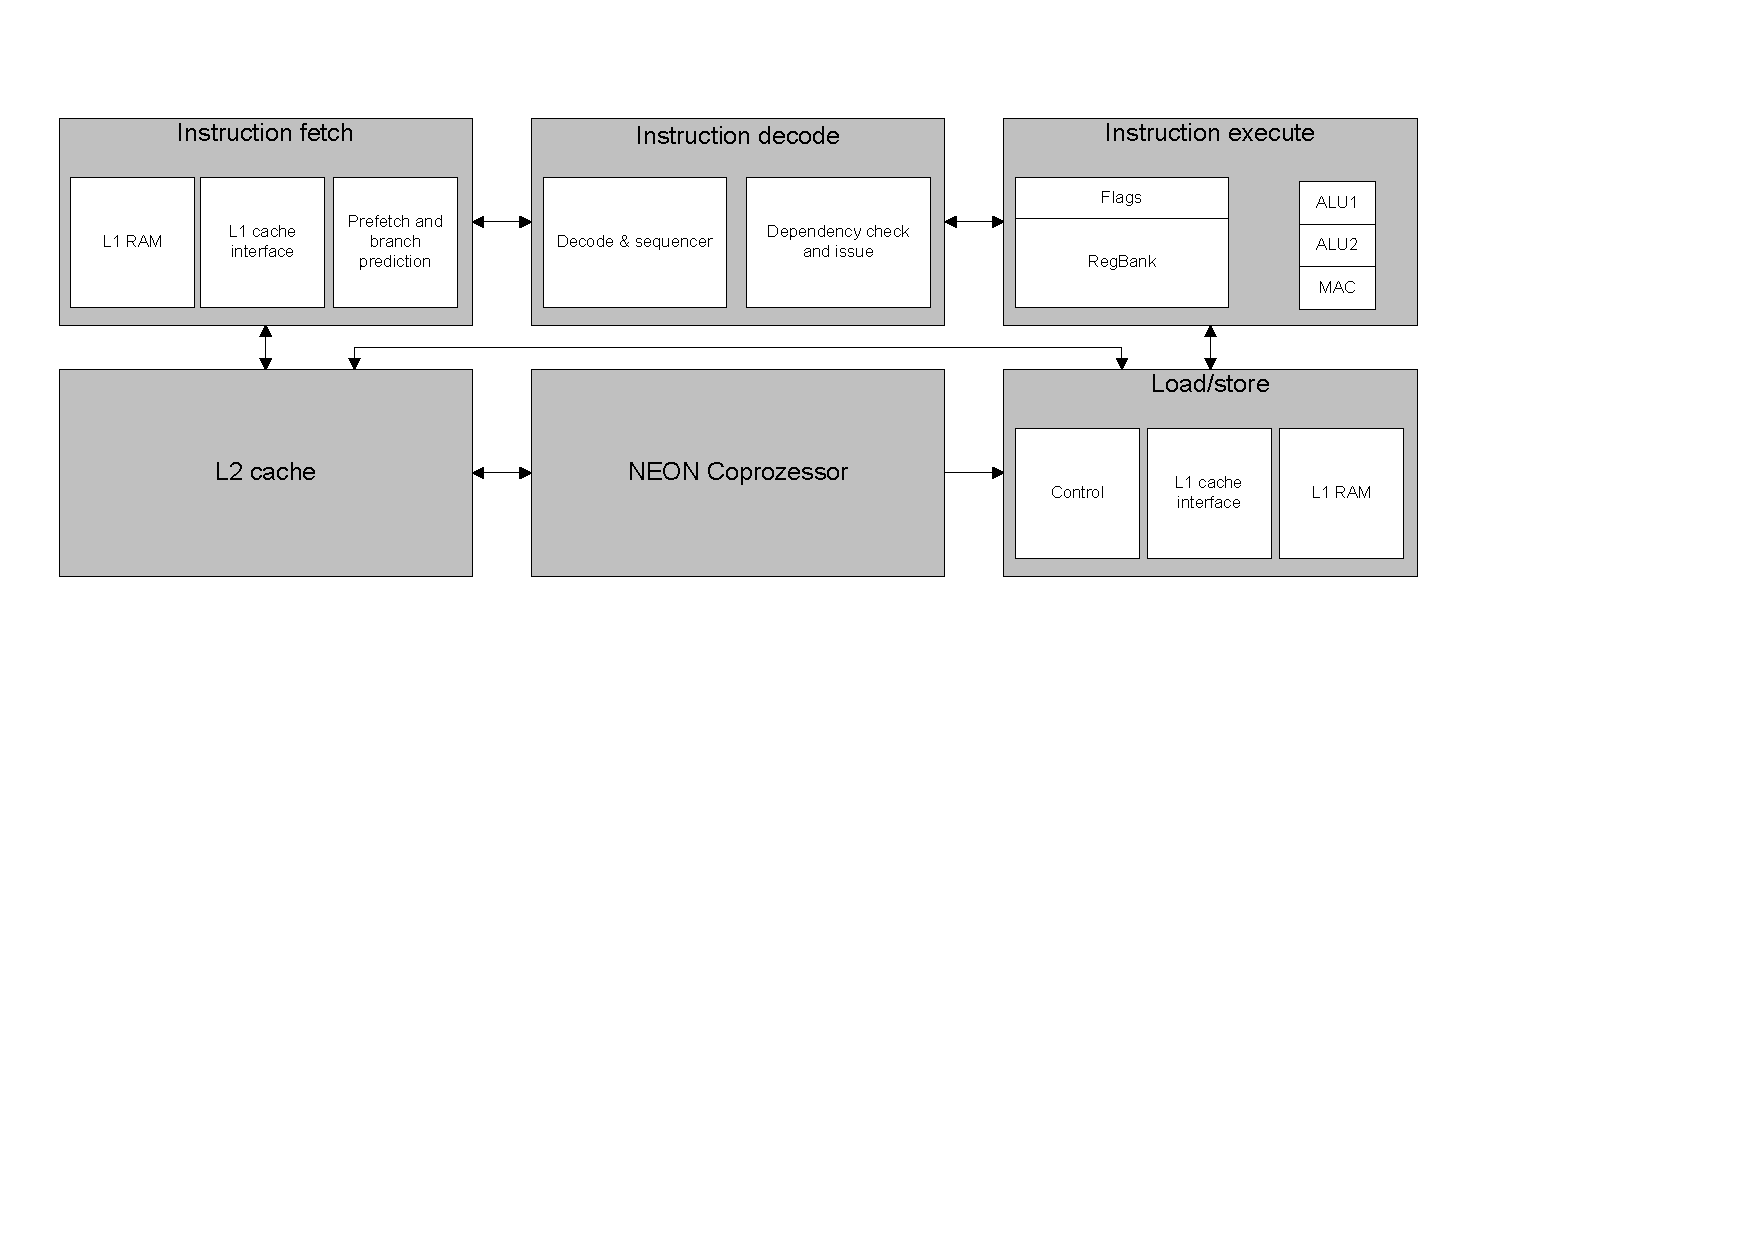
\includegraphics[width=1\textwidth]{../Pictures/cortexa8.pdf}
	\caption{Cortex-A8 Blockdiagramm\cite{cortexa8}}
	\label{fig:a8}
\end{figure} 
%
Wie in der Abbildung zu sehen ist, besteht der Cortex-A8 aus zwei wesentlichen Teilen:
\begin{itemize}
\item ARMv7 Prozessorkern (\textbf{\ref{subsubsec:armv7}})
\item NEON-Coprozessor (\textbf{\ref{subsubsec:neon}})
\end{itemize}

Diese beiden Prozessorkerne teilen sich Instruction Fetch, Instruction Decode, Instruction Execute, Load/Store und L2 Cache.\\

\subsubsection{ARMv7-A Prozessorkern}\label{subsubsec:armv7}
Der ARMv7-A Prozessorkern besitzt neben Operationen f�r Spr�nge, etc. nur Operationen f�r die Berechnung von Integerwerten.\\
Die Caches dieses Prozessorkerns besitztem folgende Eigenschaften:
\begin{itemize}
\item separate L1 Instruktions- und Datencaches
\begin{itemize}
\item Harvard Architektur
\item Gr��e von 32 KB
\item 64 Bytes Zeilenl�nge
\item vierfach assoziative Cachestruktur
\end{itemize}
\item L2 Cache
\begin{itemize}
\item Gr��e von 256KB
\item 64 Bytes Zeilenl�nge
\item achtfach assoziative Cachestruktur
\end{itemize}
\end{itemize}
Instruktionen werden in einer dreiphasigen Pipeline abgearbeitet, die wiederum in 13 Stufen unterteilt ist.\\
Die Fetch-Phase besitzt drei Stufen. In ihr werden ben�tigte Befehle aus dem L1-Instruction-Cache geladen, der sich in der Instruction Fetch-Einheit befinden (vgl. \textbf{Abbildung \ref{fig:a8}}).\\
Diese Instruktionen werden in einen Buffer geladen, welcher in der Decode-Phase, welche in f�nf Stufen unterteilt ist, ausgelesen wird und die Instruktionen decodiert werden. Au�erdem wird in der Decode-Phase die Ausf�hrungsreihenfolge der geladenen Befehle festgelegt. Diese Reihenfolge h�ngt von Datenabh�ngigkeiten und Ausf�hrungszeiten der einzelnen Operationen ab, die f�r die Ausf�hrung ben�tigt werden (eine �bersicht der Instruktionen wird im Anhang gegeben).\\
In der Execute-Phase werden anschlie�end die Befehle an die entsprechenden Funktionseinheiten weitergeleitet. Dieses geschieht in sechs Stufen.\\
Wie schon erw�hnt ist dieser Prozessorkern auf Integeroperationen ausgelegt, wird aber bei der Kompilierung eines Programms f�r den Cortex-A8 dem Compiler nicht die Benutzung einer Floating Point-Einheit vorgeschrieben (vgl. \textbf{Kapitel \ref{subsubsec:neon}}) werden auch entsprechende Befehle auf den Integeroperationen des ARMv7-A Prozessorkerns emuliert, was zu langen Ausf�hrungszeiten f�hren kann. Derartige Floating Point Instruktionen sind durch das Pr�fix \textit{\_\_aeabi\_} im Assembler-Code gekennzeichnet. Dieses bedeutet, dass Floating Point-Operationen nicht auf Hardware-, sondern auf Softwareebene berechnet werden.\\
Die \textbf{Tabelle \ref{tab:aeabi}} gibt einen �berblick �ber die in Software hinterlegten Floating Point-Operationen des ARMv7 Prozessorkerns.\\
%
\begin{table}[h]
\centering
\begin{tabular}{|c|c|}
\hline
Befehl & Beschreibung\\
\hline\hline
float \_\_aeabi\_fadd(float a, float b) & single-precision Addition\\
float \_\_aeabi\_fdiv(float n, float d) & single-precision Division, n/d\\
float \_\_aeabi\_fmul(float a, float b) & single-precision Multiplikation\\
float \_\_aeabi\_frsub(float x, float y) & single-precision umgekehrte Subtaktion, y - x\\
float \_\_aeabi\_fsub(float x, float y) & single-precision Subtraktion, x - y\\
int \_\_aeabi\_fcmpeq(float a, float b) & 1, wenn a = b\\
int \_\_aeabi\_fcmplt(float a, float b) & 1, wenn a < b\\
int \_\_aeabi\_fcmple(float a, float b) & 1, wenn a <= b\\
int \_\_aeabi\_fcmpge(float a, float b) & 1, wenn a >= b\\
int \_\_aeabi\_fcmpgt(float a, float b) & 1, wenn a > b\\
\hline
\end{tabular}
\caption{Auszug der Floating Point-Operationen des ARMv7\cite{aeabi}}
\label{tab:aeabi}
\end{table}
%
Der Instruktionssatz des ARMv7-A Prozessorkerns besitzt des weiteren Operationen die f�r die Kommunikation zwischen ihm und angeschlossenen Coprozessoren benutzt werden k�nnen. Diese Funktionen werden mir MCR und MRC bezeichnet und weisen je nach angesprochenem Coprozessor unterschiedliche Ausf�hrungszeiten auf, diese Operationen ben�tigen aber immer mindestens 60 Takte.

\subsubsection{Der NEON-Coprozessor}\label{subsubsec:neon}
Dieser Coprozessor beherbergt zwei Einheiten zur Berechnung von Floating Point-Operationen. Zum Einen ist das die VFPv3-Einheit (\textbf{\ref{ph:vfp}}) und zum Anderen die NEON-SIMD-Einheit (\textbf{\ref{ph:neon}}). 
%
\begin{figure}[h]
	\centering
		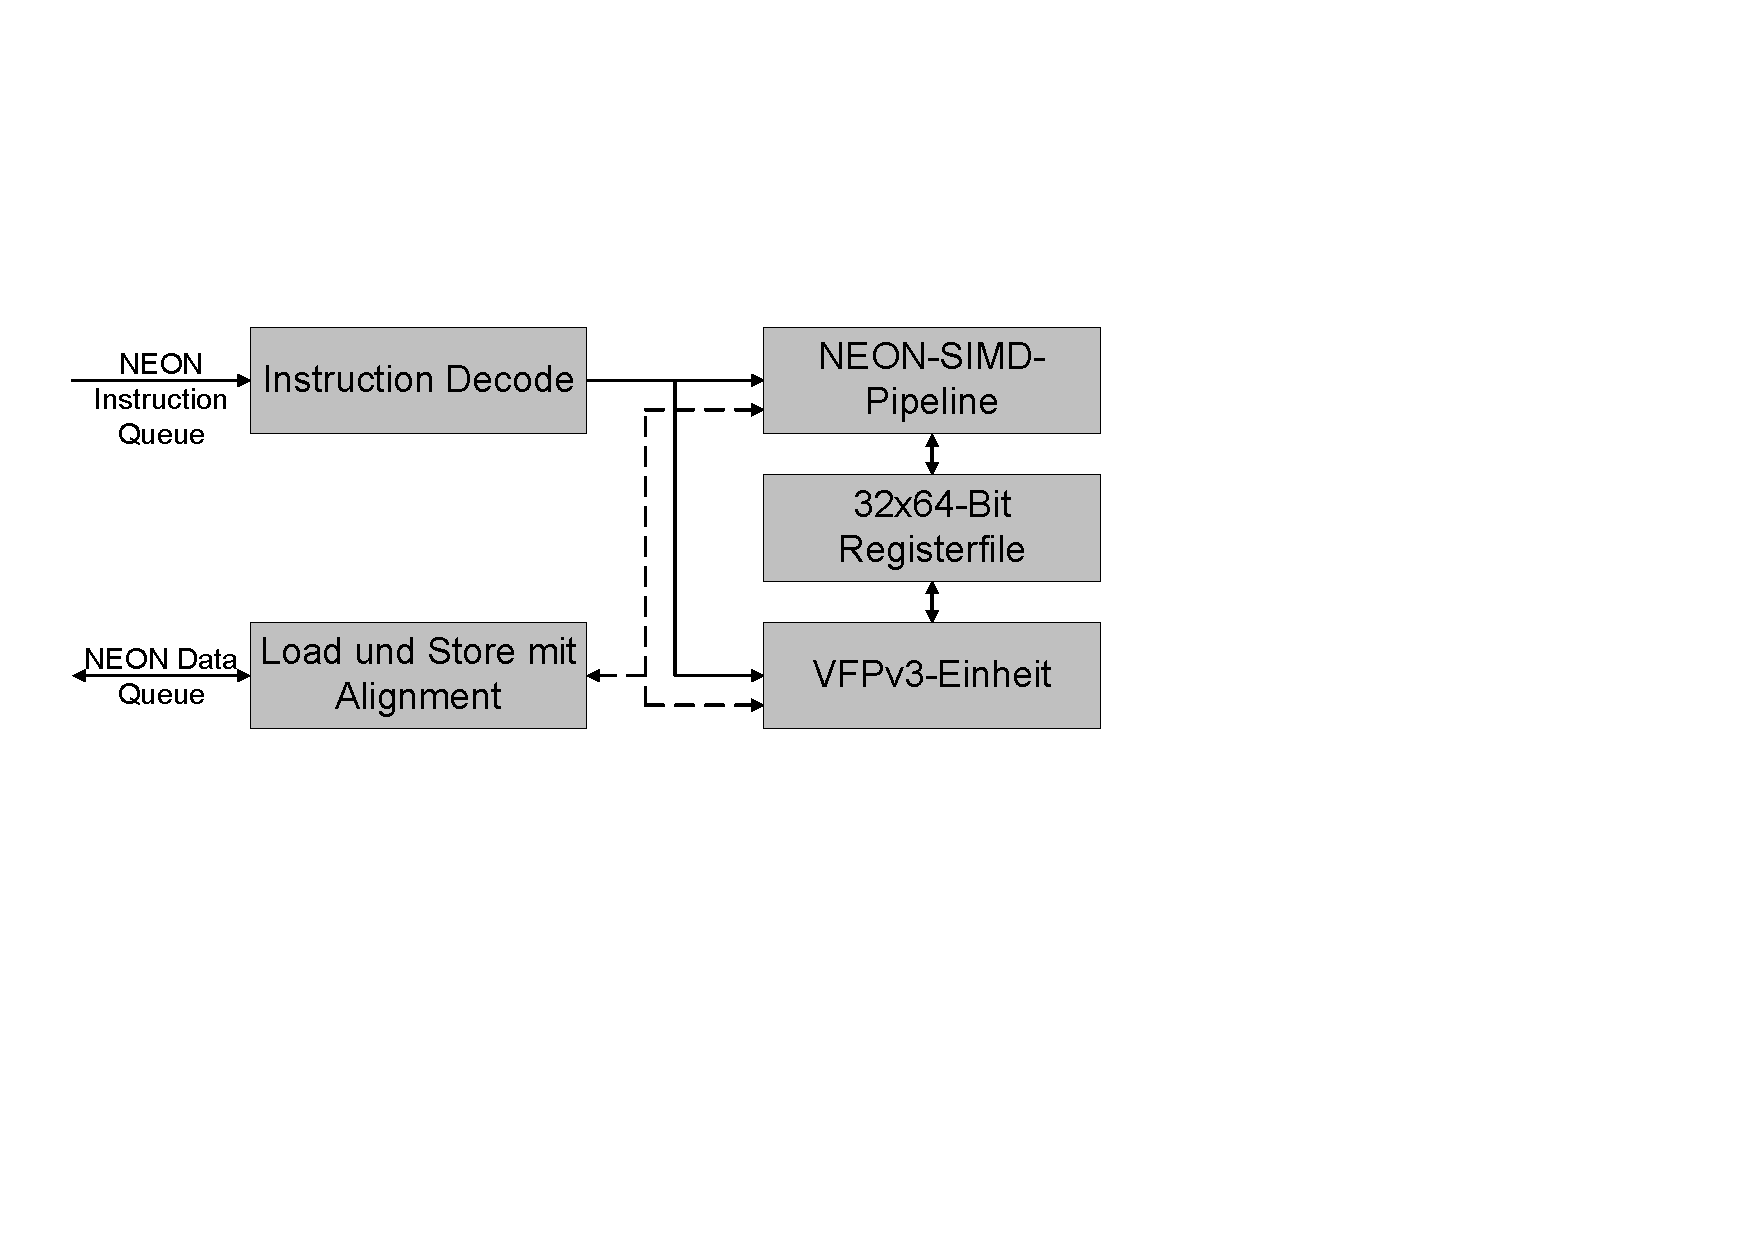
\includegraphics[scale=0.8]{../Pictures/NEON.pdf}
	\caption{Vereinfachtes Blockdiagramm des NEON-Coprozessors}
	\label{fig:neon}
\end{figure} 
%

Des weiten sind noch:
\begin{itemize}
\item Eine NEON-Registerbank mit 32x64-bit General-purpose Registern,
\item eine NEON Integer Execute Pipeline (ALU,Shift,MAC),
\item eine NEON Double- und Single-Precision Floating Point Execute Pipeline (FADD, FMUL)
\item und eine NEON Load/Store und Permute Pipeline vorhanden.
\end{itemize}
Die 32x64-bit Register liegen in einer Registerbank, die unabh�ngig von der Registerbank des ARMv7 Prozessorkerns ist, \textbf{Abbildung \ref{fig:neonbank}} zeigt die Sicht von der VFPv3- und der NEON-SIMD-Einheit auf dieses Register.\\
%
\begin{figure}[h]
	\centering
		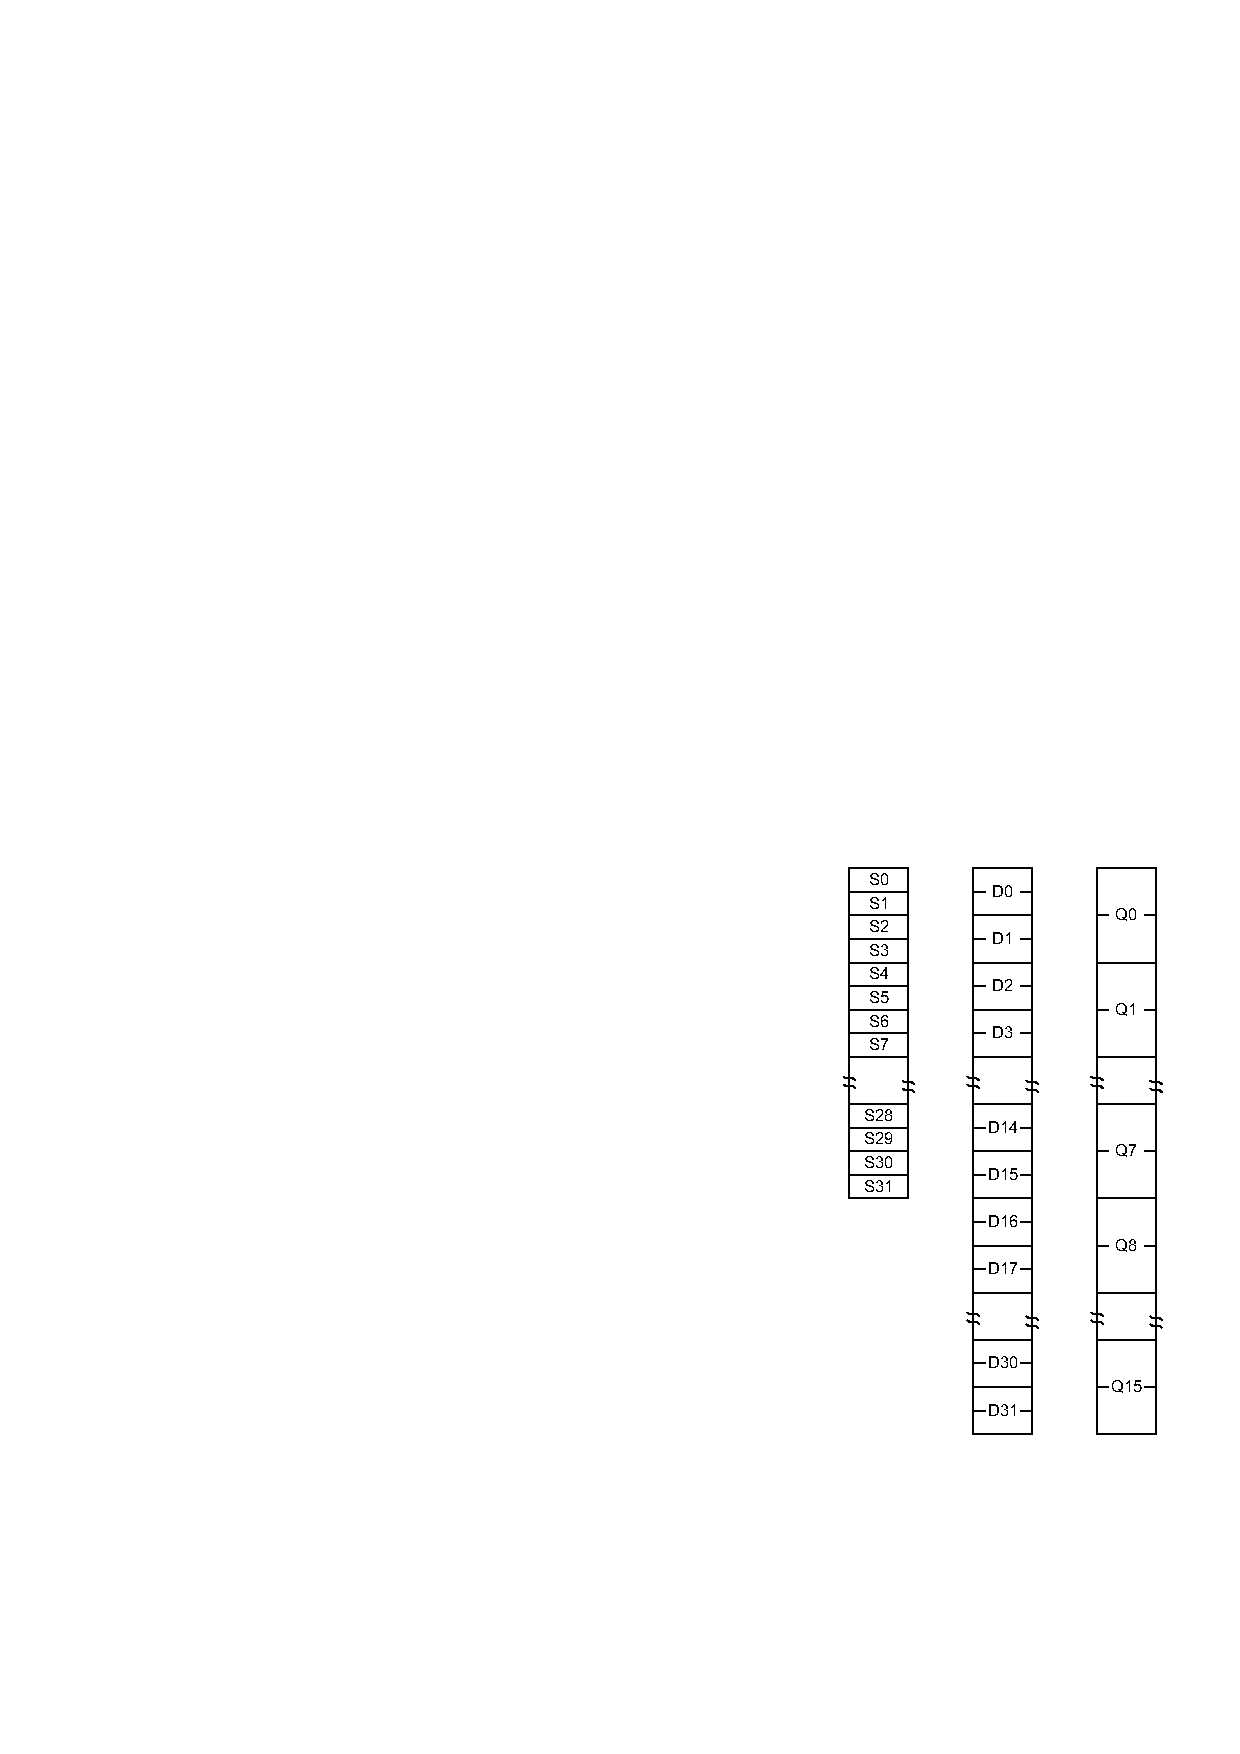
\includegraphics[scale=0.8]{../Pictures/neonbank.pdf}
	\caption{Register der NEON-SIMD- und der VFPv3-Einheit\cite{cortexa8}}
	\label{fig:neonbank}
\end{figure} 
%
Die Kommunikation zwischen ARM und NEON-Einheit geschieht l�sst sich in zwei Teile unterteilen:
\begin{itemize}
\item Weiterleitung von Befehlen
\item Weiterleitung von Daten
\end{itemize}

Die Weiterleitung von Befehlen vom ARM zum NEON-Coprozessor geschieht in folgenden Schritten:

\begin{enumerate}
\item NEON-SIMD- und VFPv3-Befehle durchlaufen die gesamte ARM-Pipeline und werden am Ende der Execute-Phase in eine NEON Instruction Queue geladen, welche 16 Eintr�ge halten kann. Danach gelten die NEON- und VFPv3-Befehle als abgearbeitet und er kann wieder ARM-Befehle ausf�hren. Eine Ausnahme bildet hier der Fall, dass die 
\item Der NEON-Coprozessor lie�t aus dieser Queue und muss die Befehle nochmals Dekodieren und ihre Abarbeitungsreihenfolge festlegen NEON Instruction Queue voll ist. Sollte dieses geschehen muss der ARM warten bis wieder Eintr�ge in diese Queue geschrieben werden k�nnen.
\item Die NEON-SIMD- und VFPv3-Befehle werden auf dem NEON-Coprozessor verarbeitet
\item Mit dem MRC-Befehl lie�t der ARM die Ergebnisse des NEON-Coprozessors aus, dieses dauert mindestens 20 Takte
\end{enumerate}

Die Weiterleitung von Daten an den NEON-Coprozessor kann auf zwei Arten geschehen:

\begin{itemize}
\item Der ARM Prozessor schreibt mit dem MCR-Befehl Daten in die NEON Daten Queue, welch e12 Eintr�ge halten kann
\item oder der NEON-Coprozessor lie�t direkt aus dem L2 Cache.
\end{itemize}

Obwohl sich die NEON- und die VFP3-Einheit einige Befehle und die Registerbank teilen, haben sie doch entscheidende Unterschiede, die in den beiden folgenden Kapiteln erl�utert werden sollen.

\paragraph{VFPv3-Einheit}\label{ph:vfp}$\;$ \\\\
Die VFPv3-Einheit stellt einen Coprozessor, welcher auf der \textit{VFPv3-Architektur} basiert, zur Berechnung von Floating Point-Zahlen zur Verf�gung und unterst�tzt den \textit{ANSI/IEEE Standard 754-1985} in vollem Umfang.\\
Hierf�r stellt die VFPv3-Einheit Operationen zur Addition, Subtraktion, Multiplikation, Division, Multiply-and-Accumulate und zur Wurzelberechnung zur Verf�gung, die sowohl mit Single-Precision als auch Double-Precision berechnet werden k�nnen. Des weiteren werden Operationen zur Konvertierung zwischen Floating- und Fix-Point und Floating-Point und Konstanten bereitgestellt.\\
Die VFPv3-Einheit besitzt keine Pipeline-Struktur und ist nur in der Lage Anweisungen sequenziell abzuarbeiten.\\
Sie hat auf die in \textbf{Abbildung \ref{fig:neonbank}} abgebildete Registerbank Zugriff wie folgt:

\begin{itemize}
\item Als 32 32-bit Einzelwortregister, S0-S31, in dieser Sicht ist nur die halbe Registerbank zugreifbar,
\item Als 32 64-bit Doppelwortregister, D0-D31
\item und als Kombination dieser 32- und 64-bit Register
\end{itemize}

In \textbf{Tabelle \ref{tab:vfp}} sind wesentliche Instruktionen aus dem Instruktionssatz der VFPv3-Einheit mit Angabe der Ausf�hrungszeit in Takten gegeben. Hierbei ist zu erw�hnen, dass diese Ausf�hrungszeiten datenabh�ngig sind.

\begin{table}
\centering
\begin{tabular}{|c|c|c|}
\hline
Befehl & Single-Precision-Takte & Double-Precision-Takte\\
\hline\hline
FADD & 9-10 & 9-10\\
FSUB & 9-10 &9-10\\
FMUL \& FNMUL & 10-12 & 11-17\\
FMAC \& FNMAC & 18-21 & 19-26\\
FDIV & 20-37 & 29-65\\
FSQRT & 19-33 & 29-60\\
FABS & 4 & 4\\
FCMP & 4 oder 7 & 4 oder 7\\
FCPY & 4 & 4\\
\hline
\end{tabular}
\caption{Auszug aus dem Instruktionssatz der VFPv3-Einheit\cite{cortexa8}}
\label{tab:vfp}
\end{table}

\paragraph{NEON-SIMD-Einheit}\label{ph:neon}$\;$ \\\\
Die NEON-SIMD-Einheit ist eigentlich f�r die Ausf�hrung von Integeroperationen konzipiert, kann aber ebenfalls Floating Point-Operationen ausf�hren.\\
Diese Einheit basiert auf der \textit{Advanced SIMD Media Processing-Architektur}. SIMD steht hierbei f�r \textit{Single Input Multiple Data} und hei�t, dass ein und der selbe Befehle gleichzeitig auf mehrere Eingangsdaten angewendet werden kann. Der NEON-SIMD-Einheit ist es m�glich pro Operand 128 Bit gleichzeitig einzulesen und zu schreiben, allerdings kann sie nur 64 Bit gleichzeitig verarbeiten, woraus folgt, dass immer zwei Operationen parallel ausgef�hrt werden k�nnen.\\
Auch die NEON-SIMD-Einheit verwendet die in \textbf{Abbildung \ref{fig:neonbank}} abgebildete Registerbank und kann Operationen auf dieser mit folgenden Ein- und Ausgaberegistern ausf�hren:

\begin{itemize}
\item Mit 16 128-bit Quadwortregistern, Q0-Q15,
\item mit 32 64-bit Doppelwortregistern,D0-D31, die auch von der VFPv3-Einheit sichtbar sind
\item und mit Kombinationen aus den 128- und 64-bit Registern.
\end{itemize}
Die Einheit kann bis zu zwei Advanced SIMD Operationen pro Takt von der Integer Execution Einheit des ARMs empfangen und zus�tzlich noch 32-bit MCR oder MRC Daten mit dieser tauschen.\\
Des weiten werden NEON-SIMD-Befehle in einer 10-stufigen Pipeline abgearbeitet.\\
Au�erdem ist es der NEON-SIMD-Einheit m�glich Teile der VFPv3-Befehle in ihrer Pipeline auszuf�hren um die Abarbeitungszeit zu beschleunigen.\\
In \textbf{Tabelle \ref{tab:neon}} ist ein Auszug des NEON-SIMD-Befehlssatzes mit Ausf�hrungszeiten in  Takten angegeben. Sigle-Precision-Befehle sind im sp�teren Assemblercode durch den Zusatz \textit{.f32} hinter dem Befehlsnamen gekennzeichnet.

\begin{table}[hpt]
\centering
\begin{tabular}{|c|c|c|}
\hline
Befehl & Takte\\
\hline\hline
VADD & 1-2\\
VSUB & 1-2\\
VMUL & 1-2\\
VABS & 1-2\\
VRSQRT&1-2\\
VMLA&1-2\\
VMLS&1-2\\
VMOV & 1\\
VLDR  & 1-2\\
VSTR  & 1-2\\
\hline
\end{tabular}
\caption{Auszug aus dem Floating Point-Befehlssatz der NEON-SIMD-Einheit\cite{cortexa8}}
\label{tab:neon}
\end{table}

\subsubsection{Ansteuerungsm�glichkeiten}
Wird beider Kompilierung nicht spezifiziert, wie Floating Point-Operationen behandelt werden sollen, werden diese immer mit den in \textbf{Tabelle \ref{tab:aeabi}} angegeben Softwarefunktionen emuliert.\\
Sollen solche Operationen auf der VFPv3-Einheit ausgef�hrt werden muss lediglich das Flag \textit{\-mfpu=vfp} gesetzt werden.\\
Die NEON-SIMD-Einheit kann auf den �blichen vier wegen Angesprochen werden:
\begin{itemize}
\item Ansteuerung durch den Compiler
\item Unterst�tzung des Compilers durch Umstrukturierung des Codes
\item Einf�gen von Intrinsics in den Code
\item Algorithmen direkt in NEON-Assembler schreiben
\end{itemize}
Da diese vier Optionen f�r die sp�tere Optimierung verwendet werden, soll zu jeder dieser Varianten auch noch ein Beispiel gegeben werden. Wichtig ist, dass bei allen vier Varianten das Compilerflag \textit{-mfpu=neon} gesetzt sein muss.
 
\paragraph{Compiler}\label{ph:neoncomp}$\;$ \\\\
Die erste Variante ist die am leichtesten Umzusetzende. Hierbei wird nur das vorher erw�hnte Compilerflag gesetzt und der Compiler f�gt w�hrend der Kompilierung an ihm sinnvoll erscheinenden Stellen NEON-Assembler-Code ein.\\
Als Beispiel soll hier ein einfacher Beipielcode verwendet werden der in den \textbf{Listings \ref{code:spfc} - \ref{code:spfneon}} in C, ARM-Assembler und in ARM+NEON-Assembler angegeben wird.

\begin{lstlisting}[caption=1. einfaches Beispiel in C, label=code:spfc]
 int i;
 for (i = 0; i < 200; i++) {
 z[i] = a[i] * b[i];
 }
\end{lstlisting}

\begin{lstlisting}[caption=ARM-Assembler, label=code:spfarm]
	PUSH     {r4,r5,lr}
	MOV      r3,#0
|L1.8|:
	ADD      r4,r0,r3,LSL #1
	ADD      r5,r1,r3,LSL #1
	LDRH     r4,[r4,#0]		;Laden von a[i];
	LDRH     r5,[r5,#0]		;Laden von b[i];
	SMULBB   r4,r4,r5
	ADD      r5,r2,r3,LSL #1
	ADD      r3,r3,#1
	CMP      r3,#0xc8		;200 Iterationen;
	STRH     r4,[r5,#0]     ;Speichern in z[i];
	BLT      |L1.8|
	POP      {r4,r5,pc}
\end{lstlisting}

\begin{lstlisting}[caption=ARM+NEON-Assembler, label=code:spfneon]
	MOV      r3,#0x19 		;nur noch 25 Iterationen;
|L1.4|
	VLD1.16  {d0,d1},[r0]!	;Laden von a;
	SUBS     r3,r3,#1
	VLD1.16  {d2,d3},[r1]!  ;Laden von b;
	VMUL.I16 q0,q0,q1		;a*b;
	VST1.16  {d0,d1},[r2]!	;Speichern in z;
	BNE      |L1.4|
	BX       lr
\end{lstlisting}

Hierbei sieht man, dass sowohl die Lade und Speicheroperationen, als auch, dass die Multiplikation an sich parallelisiert wurden.

\paragraph{C-Code}\label{ph:neonc}$\;$ \\\\
Die zweite Variante erfordert ein Eingreifen in die Code-Struktur. Hierbei geht es darum, kritische Stellen im Code zu identifizieren und zu isolieren, die es dem Compiler nicht erlauben eine auf den NEON abbildbare Codestelle zu erkennen. Dieses kommt insbesondere bei verschachtelten Anweisungen und bei unklaren Datenabh�nigikeiten vor.

\paragraph{Intrinsics}$\;$ \\\\
Eine weitere Variante bietet das Ersetzten von Berechnungen durch Intrinsics, die die entsprechende Berechnung auf Assembler-Ebene darstellen. Eine Liste der vorhandenen Intrinsics ist in \cite{intrinsics} zu finden.\\
Eine solche Ersetzung von Berechnungen durch Intrinsics soll an einem weiteren einfachen  Beispiel in den \textbf{Listings \ref{code:hamc} - \ref{code:hamneon}} verdeutlicht werden.

\begin{lstlisting}[caption=2. einfaches Beispiel in C, label=code:hamc]
	int i;
 	for(i=0;i<200;i++) {
 	z[i] = x[i] + y[i];
 	}
\end{lstlisting}

\begin{lstlisting}[caption=2. einfaches Beipiel mit Intrinsics, label=code:hamcv]
	int i;
	uint32x4_t x4,y4; // Hier werden 128 bit Register definiert, die die Operanten halten 
	uint32x4_t z4;    // Hier wird ein 128 bit Register definiert, dass das Ergebnis h�lt 
	uint32_t *ptra = x; //x,y und z sind die Eingangs-, bzw. Ausgangsarrays 
	uint32_t *ptrb = y; 
	uint32_t *ptrz = z; 

	for(i=0; i < 200/4; i++)
	{
        x4 = vld1q_u32(ptra);  // Intrinsic um x4 mit 4 Werten von x zu laden
        y4 = vld1q_u32(ptrb);  // Intrinsic um y4 zu laden
        z4=vaddq_u32(x4,y4);   // Intrinsic um z4=x4+y4 zu addieren
        vst1q_u32(ptrz, z4);   // Speicher die 4 Ergebnisse in z
        ptra+=4; // Pointer inkrementieren
        ptrb+=4;
        ptrz+=4;
	}
\end{lstlisting}

\begin{lstlisting}[caption=ARM+NEON-Assembler, label=code:hamneon]
        add      r3, r1, #800
.L2:
        vld1.32  {d4-d5}, [r1] ;Zeile 10;
        add      r1, r1, #16
        vld1.32  {d6-d7}, [r0] ;Zeile 11;
        cmp      r1, r3
        vadd.i32 q3, q3, q2    ;Zeile 12;
        vst1.32  {d6-d7}, [r2] ;Zeile 13;
        add      r0, r0, #16
        add      r2, r2, #16
        bne      .L2
        bx       lr
\end{lstlisting}

In \textbf{Listing \ref{code:hamneon}} sind alle Instruktionen wiederzufinden, die in \textbf{Listing \ref{code:hamcv}} definiert wurden.

\paragraph{Assembler}\label{ph:neonasm}$\;$ \\\\
Als letzte Variante soll die direkte Umsetzung einer Berechnung in NEON-Assembler vorgestellt werden. Hierbei werden einzelne Methoden oder ganze Programmteile nicht in einer Hochsprache wie C/C++ geschrieben sondern in NEON-Assembler.\\
Als Beispiel soll hier eine Methode aus der FFT der Libav-Bibliothek angef�hrt werden. Die Libav-Bibliothek wird im Optimierungskapitel vorgestellt.\\
Die \textbf{Linstings \ref{code:fft4c}} und \textbf{\ref{code:fft4neon}} zeigen einmal die Methode \textit{FFT4} in C-Code und in NEON-Assembler.

\begin{lstlisting}[caption= FFT4 in C, label=code:fft4c]
static void fft4(FFTComplex *z)
{
#define BF(x, y, a, b) do {                     \
        x = a - b;                              \
        y = a + b;                              \
    } while (0)

    FFTDouble t1, t2, t3, t4, t5, t6, t7, t8;

    BF(t3, t1, z[0].re, z[1].re);
    BF(t8, t6, z[3].re, z[2].re);
    BF(z[2].re, z[0].re, t1, t6);
    BF(t4, t2, z[0].im, z[1].im);
    BF(t7, t5, z[2].im, z[3].im);
    BF(z[3].im, z[1].im, t4, t8);
    BF(z[3].re, z[1].re, t3, t7);
    BF(z[2].im, z[0].im, t2, t5);
}
\end{lstlisting}

\begin{lstlisting}[caption=FFT4 in NEON-Assembler, label=code:fft4neon]
function fft4_neon
        vld1.32         {d0-d3}, [r0,:128]

        vext.32         q8,  q1,  q1,  #1       @ i2,r3 d3=i3,r2
        vsub.f32        d6,  d0,  d1            @ r0-r1,i0-i1
        vsub.f32        d7,  d16, d17           @ r3-r2,i2-i3
        vadd.f32        d4,  d0,  d1            @ r0+r1,i0+i1
        vadd.f32        d5,  d2,  d3            @ i2+i3,r2+r3
        vadd.f32        d1,  d6,  d7
        vsub.f32        d3,  d6,  d7
        vadd.f32        d0,  d4,  d5
        vsub.f32        d2,  d4,  d5

        vst1.32         {d0-d3}, [r0,:128]

        bx              lr
endfunc
\end{lstlisting}

Hierbei werden immer zwei Berechnungen parallel durchgef�hrt. Jedes BF() in \textbf{Listing \ref{code:fft4c}} besteht aus einer Addition und einer Subtraktion, es werden also insgesamt acht Additionen und 8 Subtraktionen durchgef�hrt. Im NEON-Assembler-Code aus \textbf{Listing \ref{code:fft4neon}} befinden sich vier VADDs und vier VSUBs, die jeweils f�r 2 parallele Berechnungen stehen. Also kommen wir auch hier wieder auf acht Additionen und acht Subtraktionen.

\subsection{Der C674x-DSP-Prozessor}\label{subsec:dsp}
Der C674x-DSP der Firma Texas Instruments geh�rt zur C6000-Familie und ist VLIW DSP mit Floating Point-Hardware. \textbf{Abbildung \ref{fig:DSPblock}} zeigt das Blockdiagramm des DSPs.
%
\begin{figure}[h]
	\centering
		\includegraphics[width=1\textwidth]{../Pictures/DSPblock.pdf}
	\caption{C674x Blockdiagramm\cite{evm8168}}
	\label{fig:DSPblock}
\end{figure} 
%
\subsubsection{Hardware}
Aus \textbf{Abbildung \ref{fig:DSPblock}} lassen sich folgende Hardwarekomponenten entnehmen:
\begin{itemize}
\item C674x+ CPU
\item 32kB L1 Programm (L1P) RAM und Cache (bis zu 32kB) mit Error Detection Code (EDC)
\item 32kB L1 Daten (L1D) RAM und Cache (bis zu 32kB)
\item 256kB zusammenh�ngender L2 RAM und Cache mit Error Correction Code (ECC)
\item External Memory Controller (EMC)
\item Interleaving Domain Multiple Access (IDMA)
\end{itemize}

Die Registerarchitektur innerhalb der C674x+ CPU, ihr Instruktionssatz und die Pipelinestruktur soll im Nachfolgenden n�her erl�utert werden.

\paragraph{Registerarchitektur und Instruktionssatz}\label{ph:reginst}$\;$ \\\\
Wie ebenfalls in \textbf{Abbildung \ref{fig:DSPblock}} zu sehen ist, besitzt die C674x+ CPU zwei parallele Datenpfade, die mit Register File A und B bezeichnet sind. Beide Datenpfade sind mit je mit einer 64 Bit-Leitung an den L1D-Cache angeschlossen, k�nnen also parallel 64 Bit lesen oder schreiben.\\
Innerhalb dieser Datenpfade befinden sich acht Ausf�hrungseinheiten zur Bearbeitung von Befehlen, je vier pro Datenpfad. Jeder Ausf�hrungseinheit ist hierbei ein Teil des Instruktionssatzes zugeordnet.\\
Daraus folgt, dass im Idealfall acht Befehle parallel pro Takt ausgef�hrt werden k�nnen.\\
\textbf{Abbildung \ref{fig:Register}} zeigt den Aufbau der beiden Datenpfade Register File A und B, nicht eingezeichnet sin die beiden sogenannten Crosspaths, die es Operationen aus dem Datenpfad A erlauben ein Datum pro Takt aus Register File B zu lesen und umgekehrt. Diese Crosspaths sind im Assembler-Code durch ein X hinter der Ausf�hrungseinheit gekennzeichnet.Insgesamt besitzt der DSP 64 32 Bit-Register, je 32 in A und B.
Auch wenn einige Befehle auf mehreren Ausf�hrungseinheiten ausgef�hrt werden k�nnen, lassen sich sich diese wie folgt grob unterteilen: 
\begin{itemize}
\item .M f�hrt Multiplikationen aus,
\item .L und .S sind prim�r alle anderen arithmetischen Operationen zust�ndig
\item und .D ist prim�r f�r das Laden und Speichern von Daten verantwortlich. 
\end{itemize}
%
\begin{figure}[h]
	\centering
		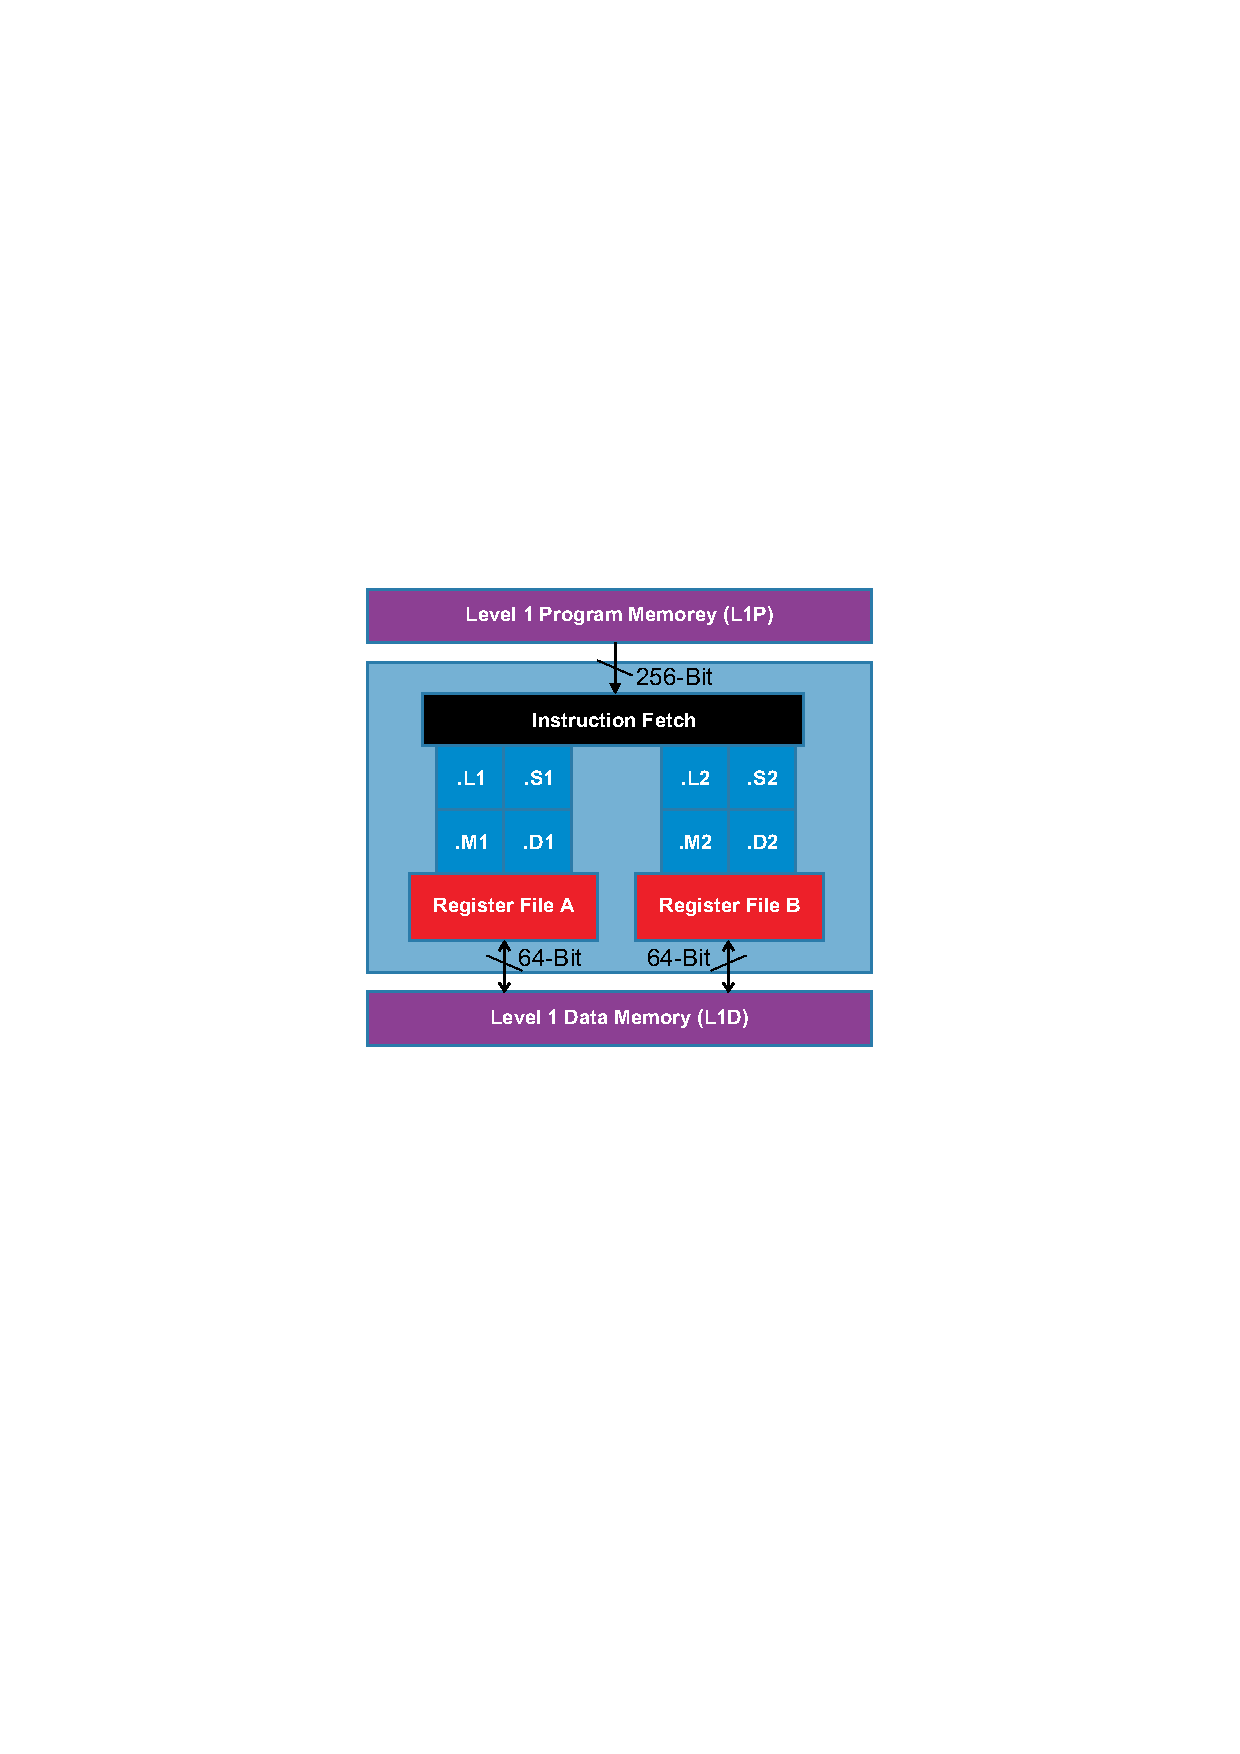
\includegraphics[scale=0.7]{../Pictures/Register.pdf}
	\caption{Stuktur der parallelen Datenpfade des C674x\cite{sprabf2}}
	\label{fig:Register}
\end{figure} 
%
\textbf{Tabelle \ref{tab:c674x}} gibt einen �berlick �ber die vorhandenen Befehle, in welcher Gruppe sie liegen, wieviele Takte sie ben�tigen und ihrer  Functional Unit Latency (FUL) und Delayslots, welche f�rs Pipelining wichtig sind. Hierbei gibt die Functional Unit Latency die Anzahl an Takten an, die eine Einheit nach Abschluss einer Berechnung ben�tigt, bis sie eine neue Berechnung annehmen kann. Die Delayslots geben die Takte an, die zwischen Einlesen der Operanden und dem Abschluss der Berechnung vergehen. Der Instruktionssatz besitzt keine Befehle f�r Divisionen oder Wurzeloperationen. Diese werden nach dem Newton-Raphson-Verfahren in Software emuliert.

\begin{table}[ht]
\centering
\begin{tabular}{|c|c|c|c|c|}
\hline
Befehl & Gruppe & Takte & Delayslots & FUL\\
\hline\hline
ADD & .D,.L\&.S & 1 & 0 & 0\\
ADDSP & .L\&.S & 4 & 3 & 1\\
ADDDP & .L\&.S & 7 & 6 & 2\\
LDW & .D & 5 & 4 & 0\\
MPY & .M & 2 & 1 & 0\\
MPYSP & .M & 4 & 3 & 1\\
MPYSPDP & .M & 7 & 6 & 3\\
MPYSP2DP & .M & 5 & 4 & 2\\
MPYDP & .M & 10 & 9 & 4\\
RSQRSP & .S & 1 & 0 & 1\\
RSQRDP & .S & 2 & 1 & 1\\
SUB & .D,.L\&.S & 1 & 0 & 0\\
SUBSP & .L\&.S & 4 & 3 & 1\\
SUBDP & .L\&.S & 7 & 6 & 2\\
\hline
\end{tabular}
\caption{Auszug aus dem Instruktionssatzssatz des C674x\cite{sprufe8b}}
\label{tab:c674x}
\end{table}

\paragraph{Pipelining auf dem C674x}\label{ph:dsppipe}$\;$ \\\\
Generell besitzt die Pipeline des C674x drei Phasen:

\begin{enumerate}
\item Fetch
\item Decode
\item Execute
\end{enumerate}

Die Fetch-Phase besitzt vier Stufen, die Decode-Phase zwei Stufen und die Execute-Phase maximal 10 Stufen (vgl. \textbf{Abbildung \ref{fig:dsppipe}}), hierbei ist eine Stufe immer einen Takt lang.
%
\begin{figure}[htb]
	\centering
		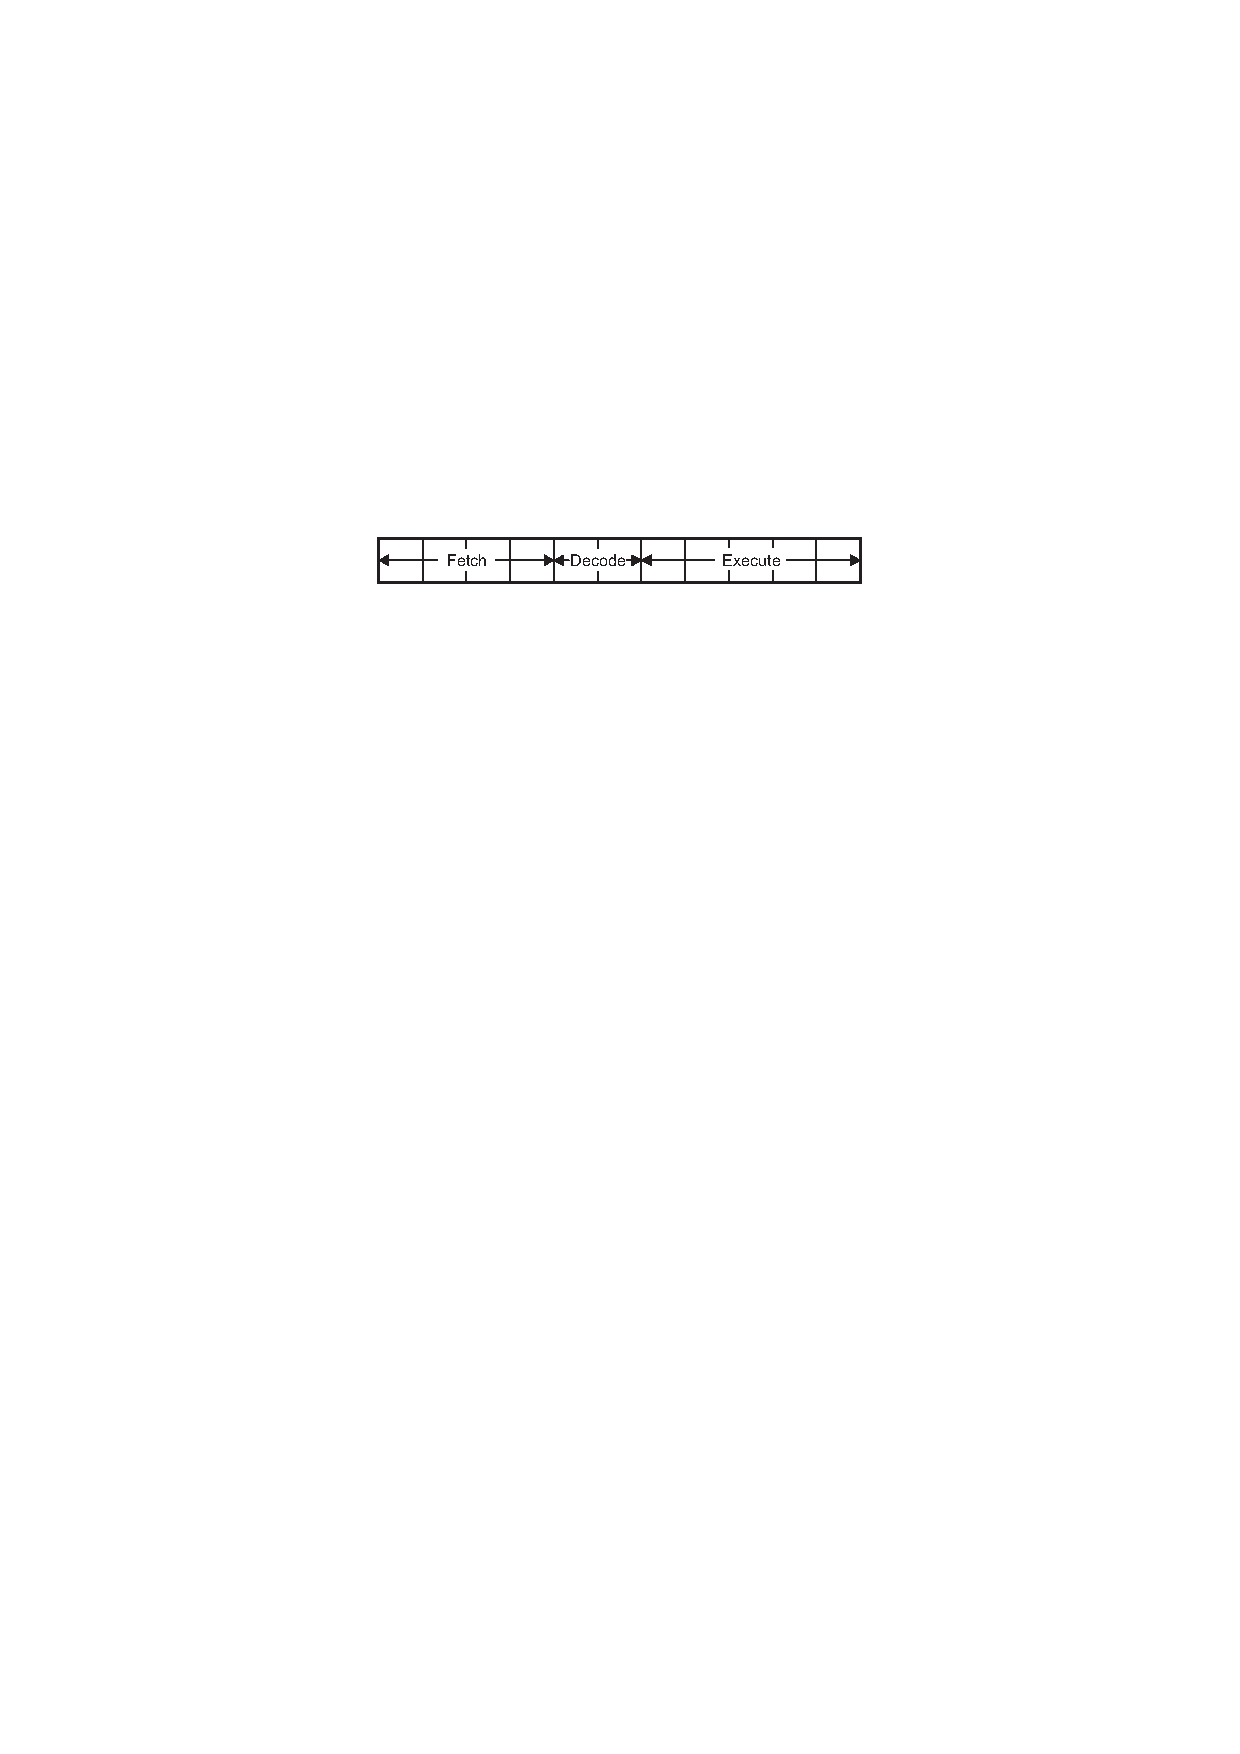
\includegraphics[width=1\textwidth]{../Pictures/dsppipe.pdf}
	\caption{Pipelinestufen und -phasen des C674x\cite{sprufe8b}}
	\label{fig:dsppipe}
\end{figure} 
% 
\subparagraph{Die Fetch-Phase}\label{subph:fetch}$\;$ \\\\
In der Fetch-Phase werden Befehle aus dem Instruktionscache geladen. Dieses ist wie bereits erw�hnt in vier Stufen unterteilt:

\begin{enumerate}
\item PG: Program address generate
\item PS: Program address send
\item PW: Program access ready wait
\item PR: Pregram fetch packet receive
\end{enumerate}

Zum Laden von Befehlen aus dem Instruktionscache wird ein sogenanntes Fetch Packet (FP) verwendet, welches aus acht Befehlen besteht. In einem Fetch Paket sind neben den acht Befehlen auch noch Informationen dar�ber enthalten, welche Befehle parallel ausgef�hrt werden k�nnen.

\subparagraph{Die Decode-Phase}$\;$ \\\\
Die Decode-Phase besteht aus zwei Stufen:
\begin{enumerate}
\item DP: Instruction dispatch
\item DC: Instruction decode
\end{enumerate}

In der DP-Phase werden die vorher geladenen Fetch Packets in sogenannte Execute Packets zerlegt. Hierbei stellt ein Execute Packet Befehle dar, die parallel auf den acht vorhandenen Ausf�hrungseinheiten bearbeitet werden k�nnen, daraus folgt, dass ein Execute Packet immer mindestens aus einem und maximal aus acht Befehlen bestehen kann. Au�erdem werden in dieser Phase den einzelnen Befehlen eines Execute Packets die Ausf�hrungseinheiten zugeordnet, die sie bearbeiten werden. Hierbei muss beachtet werden, dass Ausf�hrungseinheiten noch auf Grund von Latenzen belegt sein k�nnen (siehe \textbf{\ref{ph:reginst}}). Operationen die parallel bearbeitet werden sind im sp�teren Assembler-Code mit einem \glqq ||\grqq\  gekennzeichnet.\\
W�hrend der DC-Phase werden die Quell- und Zielregister und gegebenenfalls zugewiesene Crosspaths dekodiert, welche bei der sp�teren Ausf�hrung ben�tigt werden. 

\subparagraph{Die Execute-Phase}$\;$ \\\\
In der Execute-Stufe werden die vorher geladenen und decodierten Befehle auf den Hardwareeinheiten ausgef�hrt. Diese Stufe wird formell in zehn Stufen unterteilt, E1-E10, in denen je nach Befehl Lade- und/oder Schreiboperationen ausgef�hrt werden. Hierbei kann es allerdings passieren, dass bei manchen Befehlen eine bestimmte Zeit vergeht, bis das Ergebnis am Ausgang anliegt, diese Zeit wird als Delayslots bezeichnet und welche ab der Phase E1 gez�hlt werden (vgl. \textbf{Tabelle \ref{tab:c674x}}). Die maximale Anzahl an Delayslots im Instruktionssatz des C674x betr�gt 9.\\

\subparagraph*{Die Execute-Phase bei Double-Precision}$\;$ \\\\
Durch die Besonderheit von Double-Precision-Funktionen Operanden und Ergebnisse in zwei Schritten zu lesen, bzw. zu schreiben, ergeben sich M�glichkeiten diese beim Scheduling solcher Funktionen auszunutzen. Hierbei werden immer erst die LSBs gelesen, bzw. geschrieben und einen Takt sp�ter die MSBs.\\
Soll zum Beispiel erst eine Multiplikation (MPYSP2DP) und danach eine Addition (ADDDP) dieses Ergebnisses mit einem andern Wert geschehen, so kann die Addition bereits in dem Takt mit der Bearbeitung anfangen, in dem das LSB des Ergebnisses der Multiplikation geschrieben wurde.

\subsubsection{Code Parallelisierung durch Software Pipelined Loop (SPLOOP)}\label{ph:sploop}
Wenn Schleifen optimiert werden sollen gibt es neben Loop-Unrolling meistens keine andere M�glichkeit. Dieses Unrolling nutzt aber nicht effektiv alle acht Ausf�hrungseinheiten des DSPs aus.
Hier kommt die Software Piplined Loop ins spielt.\\ 
SPLOOP besteht zum einen Teil aus Hardware und zum anderen Teil aus Planungsarbeit, die w�hrend der Kompilierung vom Compiler aufgebracht wird.\\
Hierbei wird eine M�glichkeit geboten, Schleifen, welche im Programm vorkommen, in Form einer Pipeline abzuarbeiten. Hierf�r sind Hardwarekomponenten innerhalb des C674x vorhanden:

\begin{itemize}
\item Loop Buffer
\item Loop buffer count register (LBC)
\item Inner loop count register (ILC)
\item Reload inner loop count register (RILC)
\item Task state register (TSR)
\item Interrupt task state register (ITSR)
\item NMI/Exception task state register (NTSR)
\end{itemize}

Als erstes wird w�hrend der Kompilierung ein Ausf�hrungsplan aufgestellt, wodurch sequentiell kodierte Befehle aus verschiedenen Iterationsschritten parallel verarbeitet werden.\\
Hierf�r wird ein Iterationsschritt in sogenannte Stages unterteilt. Eine Stage bezeichnet hierbei einen Teil des sequentiell auszuf�hrenden Codes eines Interationsschritts, der sich dadurch auszeichnet, dass er eine vorgegebene Ausf�hrungszeit in Takten besitzt. Diese Ausf�hrungszeit wird als Iterationsintervall bezeichnet.\\
Wenn die Pipeline der SPLOOP vollst�ndig gef�llt ist, werden alle Stages parallel ausgef�hrt und jede Stage ist einem anderen Iterationsschritt zugeordnet. Dieses wird als Kernel bezeichnet. Die Phase vor dem Kernel wird als Prolog bezeichnet, die nach diesem als Epilog. \textbf{Abbildung \ref{fig:sploop}} soll dieses verdeutlichen.\\
%
\begin{figure}[htb]
	\centering
		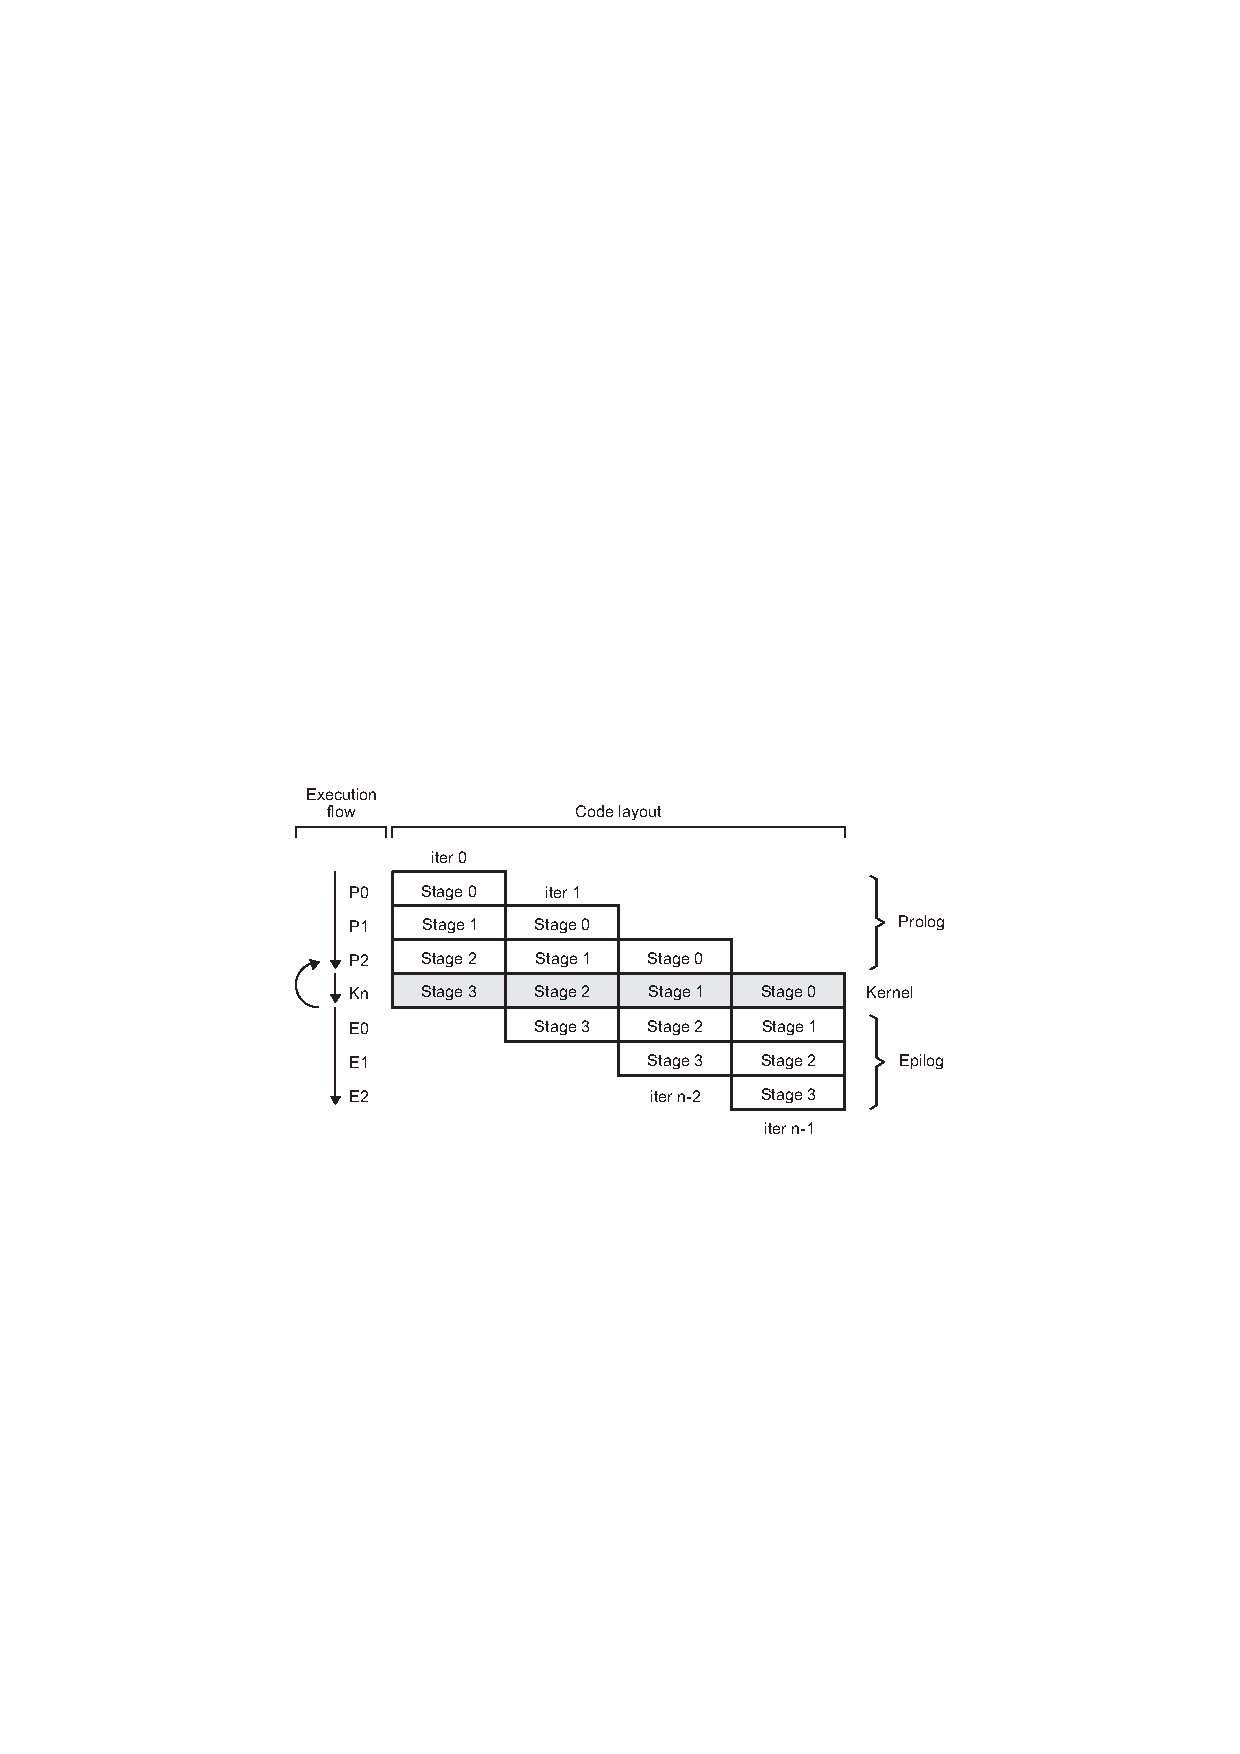
\includegraphics[width=1\textwidth]{../Pictures/sploop.pdf}
	\caption{Software Pipelined Execution Flow\cite{sprufe8b}}
	\label{fig:sploop}
\end{figure} 
% 
Um SPLOOP w�hrend der Ausf�hrung zu erm�glichen werden, SPLOOP-spezifische Befehle in den Assemblercode eingef�gt, die der zugrundeliegenden Hardware erm�glichen, Stages etc. zu erkennen. Diese Befehle lassen sich grob in drei Gruppen unterteilen:

\begin{itemize}
\item SPLOOP(D/W): Diese Befehlsgruppe l�sen den Loop Buffer Mechanismus aus
\item SPKERNEL(R): Diese Befehle markieren das Ende einer SPLOOP
\item SPMASK(R): Mit dieser Befehlsgruppe lassen sich einzelne Operationen auf Ausf�hrungseinheiten innerhalb eines Execute Packets sperren
\end{itemize}

\paragraph{Loop Buffer}$\;$ \\\\
Im Loop Buffer werden die f�r die Schleife ben�tigten Instruktionen, Informationen, ob diese momentan aktiv oder inaktiv sind und Informationen �ber ihre Abarbeitungsreihenfolge gespeichert. Diese Instruktionen werden in Form von Execute Packets gespeichert und es k�nnen bis zu 14 solcher Pakete hinterlegt werden.\\
Die Speicherung von Instruktionen im Loop Buffer bietet den Vorteil, dass sie nicht f�r jede Ausf�hrung neu die Fetch-Stufe durchlaufen m�ssen, sondern einfach aus dem Loop Buffer geladen werden k�nnen.\\
Aus diesem Buffer lie�t die Hardwareeinheit, der SPLOOP, die die parallele Abbarbeitung erm�glicht.

\paragraph{Loop buffer count register (LBC)}$\;$ \\\\
Das LBC fungiert als Inhaltsverzeichnis f�r den Loop Buffer und gibt an, welche Stages ausgef�hrt werden m�ssen. Das LBC wird in zwei F�llen auf null zur�ckgesetzt. Entweder wenn ein Befehl aus der SPLOOP(D/W)-Befehlsgruppe ausgef�hrt wird, oder wenn der Iterationsintervall-Wert erreicht ist, der beim letzten Befehl der eben genannten Gruppe mit �bergeben wurde. Sollte der zweite Fall eintreten, wird das ILC um 1 dekrementiert.\\
Es sind zwei LBCs vorhanden um eine Unterst�tzung f�r verschachtelte Schleifen zu gew�hrleisten.

\paragraph{Inner loop count register (ILC)}$\;$ \\\\
Im ILC ist die Gesamtzahl der Durchl�ufe hinterlegt, die f�r die Ausf�hrung der Schleife erforderlich sind. Erreicht das LBC den Iterationsintervall-Wert, wird das ILC dekrementiert, erreicht das ILC den Wert 0, endet die SPLOOP.

\paragraph{Reload inner loop count register (RILC)}$\;$ \\\\
Das RILC ist daf�r zust�ndig den ILC f�r die n�chste Ausf�hrung einer verschachtelten Schleife zur�ckzusetzen.

\paragraph{TSR, ITSR und NTSR}$\;$ \\

Diese drei Register sind f�r den Status der SPLOOP zust�ndig.\\
TSR zeigt an, ob eine SPLOOP momentan ausgef�hrt wird.\\
Sollte ein Interrupt kommen, wird der Inhalt des TSR in das ITSR kopiert.\\
Sollte ein Fehler oder ein nicht maskierbarer Interrupt auftreten, wird der Inhalt von TSR in NTSR kopiert.

\paragraph{Beispiel des Software-Pipelinings (SPLOOP)}\label{ph:bspsploop}$\;$ \\\\
Die Funktionsweise von SPLOOP soll nachfolgend am Beispiel der Schleife innerhalb der Berechnung des \textit{Spectral Centroids} erl�utert werden. \textbf{Listing \ref{code:scc}} zeigt den C-Code dieser Schleife und \textbf{Listing \ref{code:scasm}} den entsprechenden Assembler-Code.

\begin{lstlisting}[caption=C-Code der Schleife des Spectral Centroids, label=code:scc]
	for (k = 0; k < scsize; ++k) {
		weighted += A[k] * ((realv) k);
		total += A[k];
	}
\end{lstlisting}

\begin{lstlisting}[caption=Assembler-Code der Schleife des Spectral Centroids, label=code:scasm]
;** --------------------------------------------------------------------------*
$C$L1:    ; PIPED LOOP PROLOG

           SPLOOPD 4       ;12               ; (P) 
||         MV      .L1     A4,A6
||         MV      .S1X    B7,A8
||         MVC     .S2     B5,ILC

;** --------------------------------------------------------------------------*
$C$L2:    ; PIPED LOOP KERNEL

           INTSP   .L1     A8,A4             ; |2| (P) <0,0> 
||         LDW     .D1T1   *A6++,A5          ; |2| (P) <0,0> 

           NOP             2
           ADD     .S1     1,A8,A8           ; |1| (P) <0,3> Define a twin register
           NOP             1

           ADDSP   .L2X    A5,B4,B4          ; |3| (P) <0,5>  ^ 
||         MPYSP   .M1     A5,A4,A3          ; |2| (P) <0,5> 

           NOP             2
           NOP             1
	
           SPKERNEL 1,2
||         ADDSP   .L1     A3,A7,A7          ; |2| <0,9>  ^ 

;** --------------------------------------------------------------------------*
$C$L3:    ; PIPED LOOP EPILOG
;** --------------------------------------------------------------------------*
\end{lstlisting}
In diesem speziellen Beispiel ist der Epilog leer, dieses gilt aber nicht f�r die Allgemeinheit.\\
Wie durch den Befehl \textit{SPLOOPD 4} angegeben ist, betr�gt die L�nge eines Iterationsintervals vier Takte. Des weiteren sind sechs Stages vorhanden (innerhalb des Codes durch Leerzeilen getrennt), die jeweils vier Takte lang sind. Die einzige Ausnahme ist der Befehl \textit{LDW}, dieser wird in f�nf Takten ausgef�hrt, da allerdings nicht direkt nach dem 5. Takt aus A5 gelesen wird, stellt das kein Problem dar. Der Befehl \textit{SPKERNEL} markiert das Ende des Kernels, die Argumente dieses Befehls geben an, wie lange nach dem letzten Durchlauf gewartet werden muss, bis wieder Operationen ausgef�hrt werden k�nnen, in diesem Fall muss die Laufzeit einer Stage und 2 Takte gewartet werden, also insgesamt 6 Takte.\\
Die Konstante \textit{scsize} steht f�r die halbe Breite eines betrachteten Fensters. Die Berechnung der Gesammtlaufzeit einer Schleife mit SPLOOP wird nach \textbf{Formel \ref{eqn:sploop}} berechnet. Im Fall des \textit{Spectral Centroids} mit einer Fensterbreite von 512, betr�gt die Gesamtlaufzeit in Takten 976.

\begin{equation}\label{eqn:sploop}
Zeit~=~ \left[\overbrace{\#Stages}^{Einschwung}+\overbrace{\left(\frac{\#Durchl"aufe - 2 \cdot \#Stages}{\#Stages}\right)}^{Eingeschwungen}+\overbrace{\#Stages}^{Ausschwung}\right] \cdot Iterationsinterval
\end{equation}

\subsubsection{Compileroptimierungsstufen}
In diesem Kapitel sollen die Optimierungsstufen des DSP-Compilers aus dem bereits vorgestellten C6EZRun-Framework (siehe \textbf{Kapitel \ref{sec:c6run}}) erl�utert werden.\\
Da dieser Compiler auf dem C6000-DSP-Compiler aufsetzt, k�nnen auch die Compileroptimierungen des C6000-Compilers verwendet werden, Diese Optimierungsstufen optimieren auf Geschwindigkeit.\\
Dieser besitzt neben den g�ngigen Optimierungsstufe O0-O3, auch die M�glichkeit eine softwarebasierte Pipelinestruktur zu verwenden, die sich Software Pipelined Loop oder kurz SPLOOP nennt.

\paragraph{Optimierungsstufe \-O0}$\;$ \\\\
In der niedrigsten Optimierungsstufe, welche entweder durch das Compilerflag \textit{\-opt\_level=0} oder \textit{\-O0} aufgerufen wird, werden nur einfache Optimierungen des Codes durchgef�hrt:

\begin{itemize}
\item Kontrollfluss-Graph-Vereinfachung
\item Allokierung von Variablen auf Register
\item Loop Rotation 
\item Eliminierung von unbenutztem Code
\item Vereinfachung von Ausdr�cken und Statements
\item Unterst�tzung von Inline-Funktionen 
\end{itemize}

\paragraph{Optimierungsstufe \-O1}$\;$ \\

Die n�chst h�here Optimierungsstufe wird mit dem Compilerflag  \textit{\-opt\_level=1} oder \textit{\-O1} aufgerufen. Diese Stufe schlie�t alle Optimierungen der Stufe 0 ein und erweitert diese um:

\begin{itemize}
\item Durchf�hrung von lokalen Kopier- und Konstantenpropagation
\item Entfernung von �berfl�ssigen Anweisungen
\item Lokale Eliminierung von mehrfach verwendeten Ausdr�cken
\end{itemize}

\paragraph{Optimierungsstufe \-O2}$\;$ \\

Die Optimierungsstufe 2 wird mit dem Compilerflag \textit{\-opt\_level=2} oder \textit{\-O3} aufgerufen und erweitert die Optimierungsstufe 1 um:

\begin{itemize}
\item Optimierung f�r Verwendung der Software Pipelined Loop (\textbf{\ref{ph:sploop}})
\item Schleifenoptimierung
\item Eliminierung von globalen verbreiteten Ausdr�cken
\item Eliminierung von globalen �berfl�ssigen Ausdr�cken
\item Konvertierung von Arrayreferenzen in Schleifen zu Pointerarithmetik
\item Loop Unrolling
\end{itemize}

\paragraph{Optimierungsstufe \-O3}\label{ph:o3}$\;$ \\

Die letzte Optimierungsstufe wird mit \textit{\-opt\_level=3} oder \textit{\-O3} aufgerufen. Auch diese schlie�t alle Optimierungen der vorherigen Stufen ein, au�erdem kommen folgende dazu:

\begin{itemize}
\item Entfernung von unverwendeten Funktionen
\item Vereinfachung von Funktionen, deren R�ckgabewert nie verwendet wird
\item Inline Calls zu kleinen Funktionen
\item Neusortierung von Funktionsdeklarationen
\item Propagierung von Argumenten in den Funktionsk�rper, wenn alle Aufrufe den selben Wert an der selben Position besitzen
\item Identifizierung von File-Level Charakteristiken von Variablen
\end{itemize}

\paragraph{Beispiel der Compileroptimierung}\label{ph:bspcomp}$\;$ \\\\
Anhand des \textit{Root Mean Square} soll hier die Optimierung O3 des C6EZRun-Compilers verdeutlicht werden. Hierf�r soll neben den Optimierungen aus \textbf{Kapitel \ref{ph:o3}} auch die Pipeline aus \textbf{Kapitel \ref{ph:dsppipe}} gezeigt werden.\\
\textbf{Listing \ref{code:rmsc}} zeigt den C-Code des \textit{Root Mean Square} und \textbf{Listing \ref{code:rmsasm}} den daraus Kompilierten Assembler-Code.

\begin{lstlisting}[caption=C-Code des Root Mean Square, label=code:rmsc]
	for (n = 0; n < rmsinfo.N; ++n) {
		mean += ((realv) signal[n] / (realv) rmsinfo.N)
		* (realv) signal[n];

	}

	rms[run] = sqrt(mean);
\end{lstlisting}

\begin{lstlisting}[caption=Assembler-Code des Root Mean Square, label=code:rmsasm]
           CMPGT   .L1     A3,0,A0           ; |1| 
||         INTSP   .L2X    A3,B10
||         MV      .S1     A3,A10            ; |2| 
   [!A0]   BNOP    .S1     $C$L2,5           ; |1| 
|| [ A0]   LDW     .D1T1   *A13++,A15        ; |2| 
	   CALL    .S1     __c6xabi_divf     ; |2| 
           MV      .L2     B10,B4            ; |2| 
           MV      .L1     A15,A4            ; |2| 
           NOP             2
           MPYSP   .M1     A15,A4,A3         ; |2| 
||         SUB     .L1     A10,1,A0          ; |1| 
   [ A0]   LDW     .D1T1   *A13++,A15        ; |2| 
|| [ A0]   B       .S1     $C$L1             ; |1| 
   [ A0]   CALL    .S1     __c6xabi_divf     ; |2| 
   [ A0]   MV      .L2     B10,B4            ; |2| 
           ADDSP   .L1     A3,A14,A14        ; |1| 
           SUB     .L1     A10,1,A10         ; |1| 
   [ A0]   MV      .L1     A15,A4            ; |2|  
	   CALLP   .S2     sqrt,B3
||         SPDP    .S1     A14,A5:A4         ; |7|   
           DPSP    .L1     A5:A4,A3          ; |7| 
           NOP             1
           STW     .D1T1   A3,*+A12[A11]     ; |7| 
\end{lstlisting}

Zur Erl�uterung der Leseweise des Assembler-Codes, sei gesagt, dass ein || am Anfang einer Zeile bedeutet, dass der folgende Befehl parallel zum Befehl der vorherigen Zeile ausgef�hrt wird. Die vierte Spalte gibt den Datenpfad und die entsprechende Ausf�hrungseinheit an, so wird zum Beispiel das \textit{Zero} aus Zeile 11 im Datenpfad 1 auf der L-Einheit ausgef�hrt, |n| steht f�r die Entsprechende Zeile aus dem C-Code in \textbf{Listing \ref{code:rmsc}} (Zeile 2 und 3 werden als Zeile 2 gewertet).\\
Wie in \textbf{Kapitel \ref{subph:fetch}} bereits erw�hnt, werden immer acht Befehle zu einem Fetch Packet zusammen gefasst, so das die 23 Befehle zu drei solchen Paketen zusammen gefasst werden k�nnen (vgl. \textbf{Tabelle \ref{tab:fetch}}).

\begin{table}[ht]
\centering
\begin{tabular}{|c|c|c|c|c|c|c|c|c|}
\hline
FP Nummer & Slot 1 & Slot 2 & Slot 3 & Slot 4 & Slot 5 & Slot 6 & Slot 7 & Slot 8\\
\hline\hline
1 & cmpgt & intsp & mv & bnop & ldw & call & mv & mv\\
2 & nop & mpysp & sub & ldw & b &call& mv &addsp\\
3 & sub & mv & callp & spdp & dpsp & nop &stw &nop\\
\hline
\end{tabular}
\caption{Fetch Pakets des Root Mean Square Assembler-Codes}
\label{tab:fetch}
\end{table}

W�hrend der Decode-Stufe werden danach Zuordnungen zu Execute Pakets durchgef�hrt, wo zum Beispiel f�r Fetch Paket 1 festgestellt wurde, dass es in f�nf solcher Execute Pakets gesplittet werden kann. Diese Execute Pakets wurden danach den Ausf�hrungseinheiten zugeordnet und in der Execute-Stufe ausgef�hrt.\\
An Optimierungen lassen sich hierzum Beispiel nennen: 
\begin{itemize}
\item Die Inline Calls zu \textit{sqrt} und \textit{\_\_c6xabi\_dif}
\item Die Konvertierung von Array-Aufrufen in Pointerarithmetiken, z.B. in Zeile 5.
\item Die Propagation von Konstanten in Register, z.B. rmsinfo.N in A0
\end{itemize} 

\subsubsection{Optimierte Bibliotheken f�r den C674x}
Texas Instruments bietet zu seinen DSPs der C6000-Reihe auch noch eine Reihe Bibliotheken an, diese enthalten Algorithmen die speziell f�r DSPs dieser Baureihe optimiert wurden. Einige dieser optimierten Bibliotheken sind im Umfang des EZSDK (siehe \textbf{Kapitel \ref{sec:ezsdk}})enthalten. Im Folgenden werden zwei dieser Bibliotheken n�her vorgestellt, zum einen die DSPLIB mit Algorithmen aus der Signalverarbeitung und zum anderen die MATHLIB mit optimierten mathematischen Funktionen.

\paragraph{DSPLIB}$\;$ \\\\
Wie schon erw�hnt ist die DSPLIB-Bibliothek eine Zusammenfassung von Algorithmen aus der Signalverarbeitung, die f�r den Gebrauch auf DSPs der C6000-Reihe optimiert wurde und direkt von Texas Instruments stammt. Diese liegen innerhalb dieser Bibliothek sowohl als C- als auch als Assembler-Code vor.

\paragraph{MATHLIB}$\;$ \\

Die MATHLIB-Bibliothek ist ebenfalls f�r die Verwendung auf DSPs der C6000-Reihe optimiert. Auch diese Bibliothek stammt von Texas Instruments. F�r diese Bibliothek liegen der Quellcode ebenfalls sowohl als C- als auch als Assembler-Code vor.\\
Die mathematischen Funktionen sind sowohl f�r Double-Precision als auch f�r Single-Precision vorhanden und bieten neben der Option einzelne Aufrufe auszuf�hren, auch die M�glichkeit Operationen auf Arrays auszuf�hren. Werden diesen Arrayoperationen zum Beispiel die Array a und b �bergeben, wird immer das n-te Element von a mit dem n-ten Element von b verrechnet.

\section{Linux EZ Software Development Kit (EZSDK)}\label{sec:ezsdk}
Das Linux EZ Software Development Kit (EZSDK) ist eine von Texas Instruments zum EVM816x-Board mitgelieferte Sammlung von wichtigen und n�tzlichen Tools. Das EZSDK (gesprochen: \textit{EasySDK}) l�sst sich grob in vier Softwaregruppen unterteilen:

\begin{itemize}
\item Board Support
\begin{itemize}
\item Kernel f�r embedded Linux Version 2.6.37
\item U-Boot (Bootloader)
\item Sammlung von Tools auf System-on-Chip-Ebene
\end{itemize}
\item Component Sources
\begin{itemize}
\item Optimierte Bibliotheken f�r den DSP
\item Kommunikationsframeworks zwischen ARM und DSP
\item DSP-Betriebssystem
\item weitere Tools
\end{itemize}
\item DSP Development Kit (DSP-Toolchain)
\item Linux Development Kit (Linux-Toolchain)
\end{itemize}

F�r diese Arbeit wurde die EZSDK-Version 5.02 verwendet.

\section{C6EZRun}\label{sec:c6run}

C6EZRun ist ein Framework, welches f�r die Kommunikation zwischen ARM und DSP entwickelt wurde. Dieses Framework nimmt dem Programmierer wesentliche Aspekte der Kommunikation zwischen diesen beiden Prozessoren ab, zum Beispiel Kommunikationswege, Latenzzeiten, Speicherverwaltung, Pointerkonvertierungen, etc.\\
Hierbei sind zwei unterschiedliche M�glichkeiten zur Kommunikation zwischen ARM und DSP vorhanden:

\begin{itemize}
\item C6Runlib
\item C6Runapp
\end{itemize}

C6runlib bietet die M�glichkeit Teile des Programmcodes auf den DSP auszulagern. Hierbei werden die entsprechenden Programmteile in C-Code geschrieben und mit dem C6Runlib-Compiler zu einer Bibliothek compiliert. Diese Bibliothek kann anschlie�end in das bestehende Projekt eingef�gt und die in ihr enthaltenen Funktionen so aufgerufen werden, als wenn sie auf dem ARM laufen w�rden.\\
C6Runapp hingegen bietet die M�glichkeit ein komplettes Programm auf dem DSP auszuf�hren, dieses aber �ber die Konsole des ARM aufzurufen. Hierf�r wird der Programm-Code ebenfalls in C-Code beschrieben und mit dem C6Runapp-Compiler kompiliert.\\
Die in dieser Arbeit verwendete Version von C6EZRun ist 0.98.

\section{Optimierung des ARM}
In diesem Kapitel sollen die Anfangsbedingungen, die Ansatzpunkte, die Konzepte der durchgef�hrten Optimierungen am ARM-Code des \textit{Music Classificators} vorgestellt werden.\\
Hierzu sollen in \textbf{Kapitel \ref{sec:fset}} zuerst die Featuresets vorgestellt werden, welche f�r die Messungen der Laufzeit des Programms verwendet wurden, aus denen in \textbf{Kapitel \ref{sec:ansatz}} die wesentlichen
Bottlenecks und Optimierungspotenziale auf dem DaVinci\texttrademark extrahiert werden sollen. \textbf{Kapitel \ref{sec:optFFT}} befasst sich daraufhin den Konzepten und der Durchf�hrung von Optimierungen der FFT.
\subsection{Laufzeitmessung des Gesammtprogramms}

\subsection{Laufzeitmessung der Extraktion}

\subsection{Ansatzpunkte und Bottlenecks}\label{sec:ansatz}

Auf Basis der in \textbf{Kapitel \ref{sec:fset}} vorgestellten Featuresets sollen nun die vor Beginn der Optimierung durchgef�hrten Laufzeitmessungen vorgestellt und er�rtert werden. Es wurden zwei unterschiedliche Messreihen durchgef�hrt, die sich in den gew�hlten Optimierungen unterscheiden, die vom Compiler zur Compilezeit automatisch durchgef�hrt werden k�nnen. F�r die erste Messreihe wurde lediglich der Compilerflag \textit{-O3} verwendet, welches f�r die h�chste automatische Compileroptimierung steht, diese Messreihe soll f�r weitere Betrachtungen als \textit{Unoptimized} bezeichnet werden. \\
Die zweite Messreihe schlie�t die in \textbf{Kapitel \ref{subsec:neon}} vorgestellte NEON-Einheit ein. Auch f�r diese Messreihe wurden keine NEON-spezifischen Optimierungen des Codes vorgenommen, sondern nur die vom Compiler angebotene Option aktiviert, den Code w�hrend des Compilings selber f�r den NEON zu optimieren, im Weiteren wird diese Messreihe als \textit{NEON Autocompiler} bezeichnet. \\
Die Laufzeitanteile der drei Programmteile \textit{Extraction}, \textit{Processing} und \textit{Classification} sind in \textbf{Abbildung \ref{fig:ResultsMCL}} dargestellt.\\
%
\begin{figure}[htbp]
	\centering
		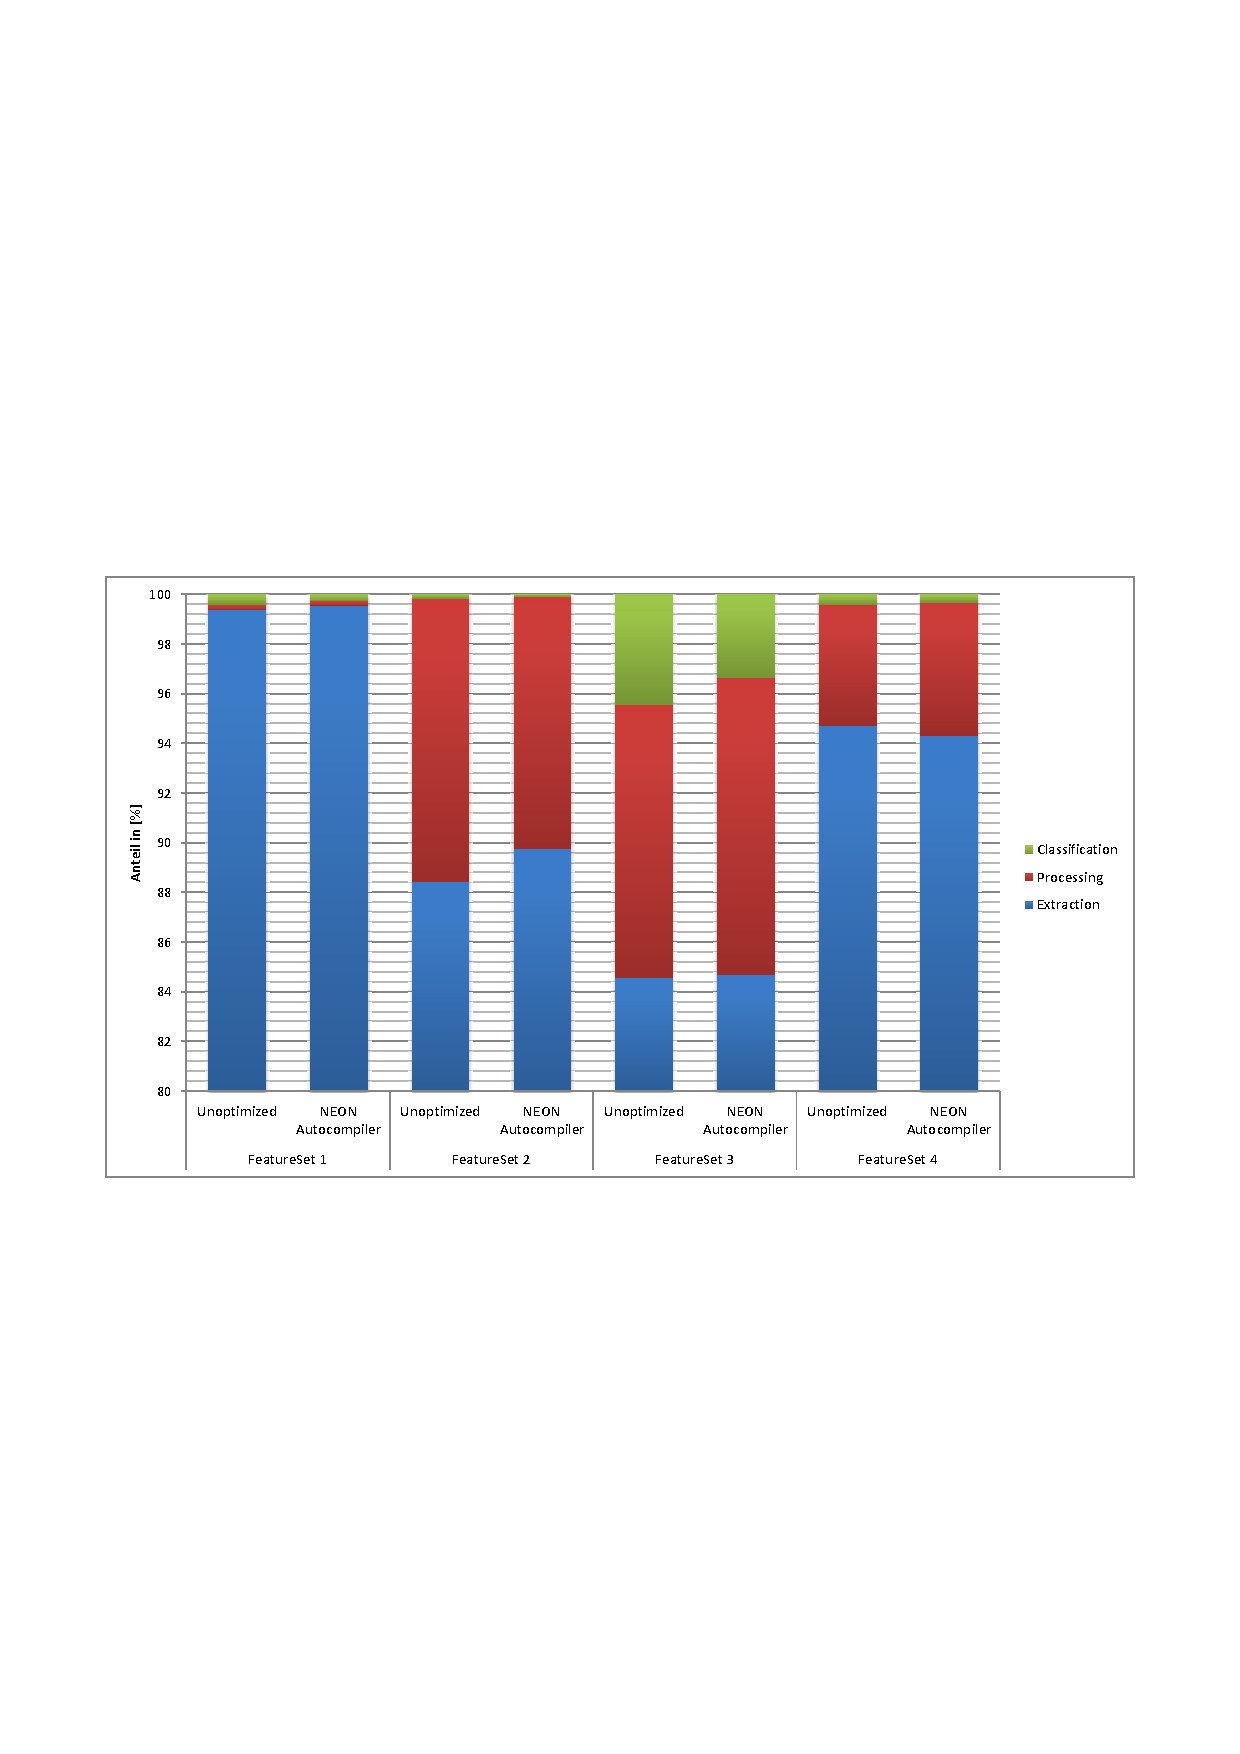
\includegraphics[width=1.00\textwidth]{../Pictures/ResultsMCL.pdf}
	\caption{Laufzeitanteile ohne manuelle Optimierung}
	\label{fig:ResultsMCL}
\end{figure}
%
Wie man leicht erkennen kann hat die Extraktion bei allen vier Featuresets mit teilweise weit �ber 80\% den gr��ten Anteil an der Laufzeit des Programms, daher wird im Nachfolgenden die Extraktion noch etwas detaillierter betrachtet werden. \\
\textbf{Abbildung \ref{fig:ResultsExtraction}} zeigt die Anteile der einzelnen Features an der Gesamtlaufzeit der Extraktion. Hier soll daran erinnert werden, dass \textit{FSet1}, \textit{FSet2} und \textit{FSet4} aus Features bestehen, die aus dem Frequenzbereich stammen, wodurch vor der Extraktion erst eine Fourier-Transformation vom Zeitbereich in diesen stattfinden muss, weshalb als weiteres "`Feature"' die FFT in der Abbildung auftaucht. Des weiteren arbeitet das Feature \textit{Ampitude of Maximum In Chromagram} aus \textit{FSet4} auf dem in \textbf{Kapitel \ref{subsubsec:cv}} vorgestellten \textit{Chroma Vector}, was dazuf�hrt, dass auch dieser in der Abbildung auftaucht.\\
%
\begin{figure}[htbp]
	\centering
		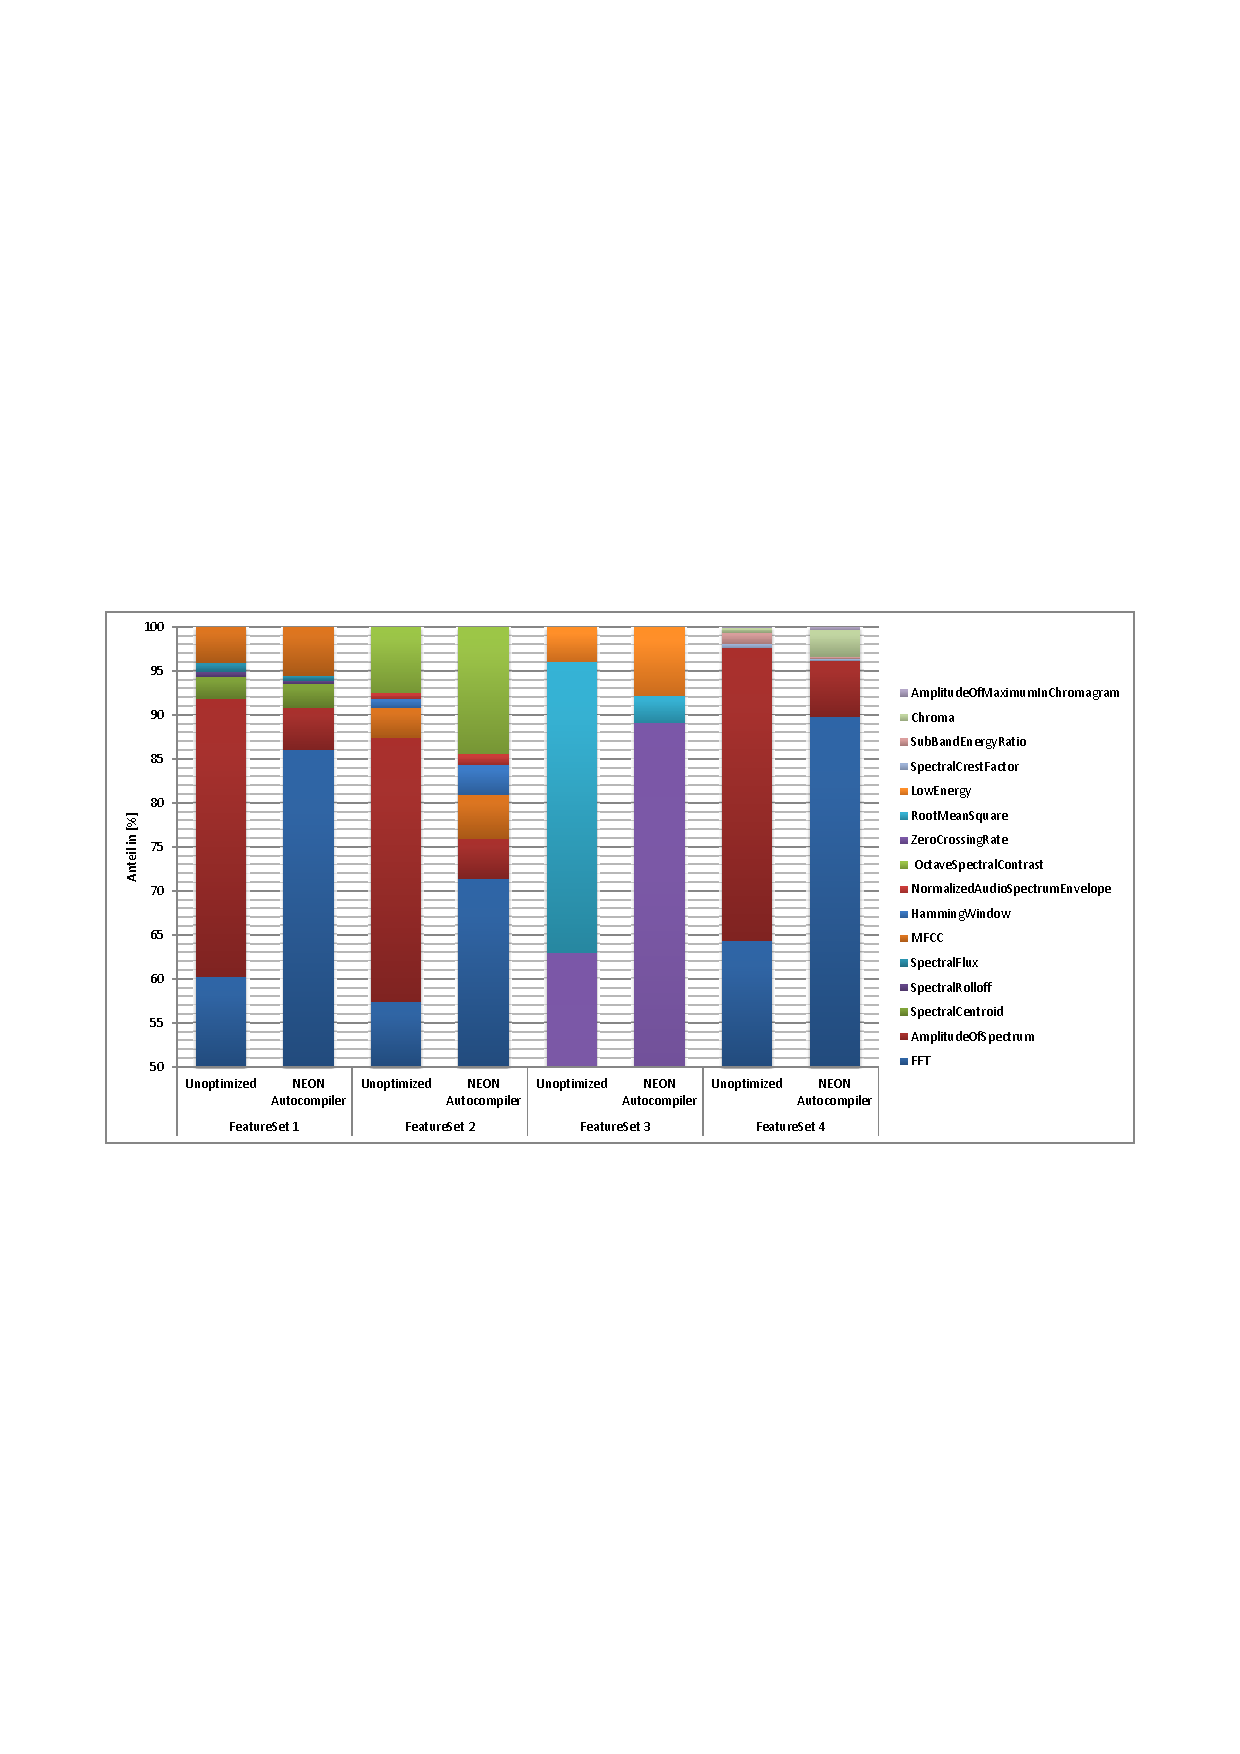
\includegraphics[width=1.00\textwidth]{../Pictures/ResultsExtraktion.pdf}
	\caption{Detaillierte Laufzeitenanteile der Extraktion ohne manuelle Optimierung}
	\label{fig:ResultsExtraction}
\end{figure}
%
Wie man der \textbf{Abbildung \ref{fig:ResultsExtraction}} entnehmen kann, hat gerade diese Transformation vom Zeit- in den Frequenzbereich den gr��ten Laufzeitbedarf, ihr Anteil liegt immer �ber 50\%. Um Irritationen zu vermeiden, soll darauf hingewiesen werden, dass sich die Laufzeit der FFT in \textit{NEON Autocompiler} nicht, wie es in der Abbildung den Anschein hat, drastisch verschlechtert hat, sondern die Verbesserungen der tats�chlichen Feature-Extraktionen sich dahingehend verbessert haben, dass die \textit{FFT} dadurch einen prozentual gr��eren Anteil einnimmt. Um genauer zu sein, hat sich in den Experimenten gezeigt, dass sich die Laufzeit der \textit{FFT} in nahezu allen F�llen fast halbiert hat.\\
Da sich gezeigt hat, dass die \textit{FFT} den gr��ten Anteil an der Laufzeit hat und das diese durch die NEON-Einheit vom Compiler schon gut optimiert werden konnte, soll im n�chsten Kapitel betrachtet werden, ob dieses durch gezielte Optimierungen bez�glich der NEON-Einheit im Code noch weiter verbessert werden kann.

\subsubsection{FFT}


\subsection{Libav als Optimierung der FFT}\label{subsec:optFFT}
\subsubsection{Laufzeitmessung}
\subsubsection{Aufbau der FFT}
\subsubsection{Einbindung}

\subsection{Optimierung der Amplitude of Spectrum}\label{subsec:optAOS}
\subsubsection{Laufzeitmessung}
\subsubsection{Codeanpassung}

\subsection{Optimierung von MFCC}

\subsection{Optimierung der Zero Crossing Rate}



 
\chapter{Optimierung des DSP-Codes}
\label{ch:optdsp}
\rm

In diesem Kapitel soll die Planung und Optimierung des DSP-Codes beschreiben werden.\\
Wie bereits in \textbf{Kapitel \ref{sec:ansatz}} gezeigt wurde, nimmt die Extraktion der zu untersuchenden Features einen Gro�teil der Laufzeit des Programmes ein.
Unter diesem Gesichtspunkt und der in \textbf{Kapitel \ref{sec:davinci}} gezeigten zugrundeliegenden heterogenen Architektur des zu betrachtenden Systems, liegt es nahe, die Extraktion auf dem DSP auszuf�hren.\\
In den nun folgenden Abschnitten sollen daher, wie schon im vorhergehenden Kapitel erst die Bottlenecks identifiziert (\textbf{\ref{sec:ansatzdsp}}) und dannach die durchgef�hrten Optimierungen beschrieben werden (\textbf{\ref{sec:mathlib}} - \textbf{\ref{sec:compiler}}).

\section{Bottlenecks des DSP-Codes}\label{sec:ansatzdsp}

F�r die Laufzeitmessungen des DSP-Codes wurden wie schon im vorherigen Kapitel die FeaturesSets 1-4 (\textbf{\ref{subsec:fset1}} - \textbf{\ref{subsec:fset4}}) verwendet.
Die ben�tigen Zeiten wurden auch hier wieder mit der Gesammtzeit in verh�ltnis gesetzt, wodurch die aus \textbf{Abbildung \ref{fig:dsp}} zu entnehmenden Anteile der einzelnen Features an der Gesammtlaufzeit errechnet wurden.

\begin{figure}
	\centering
		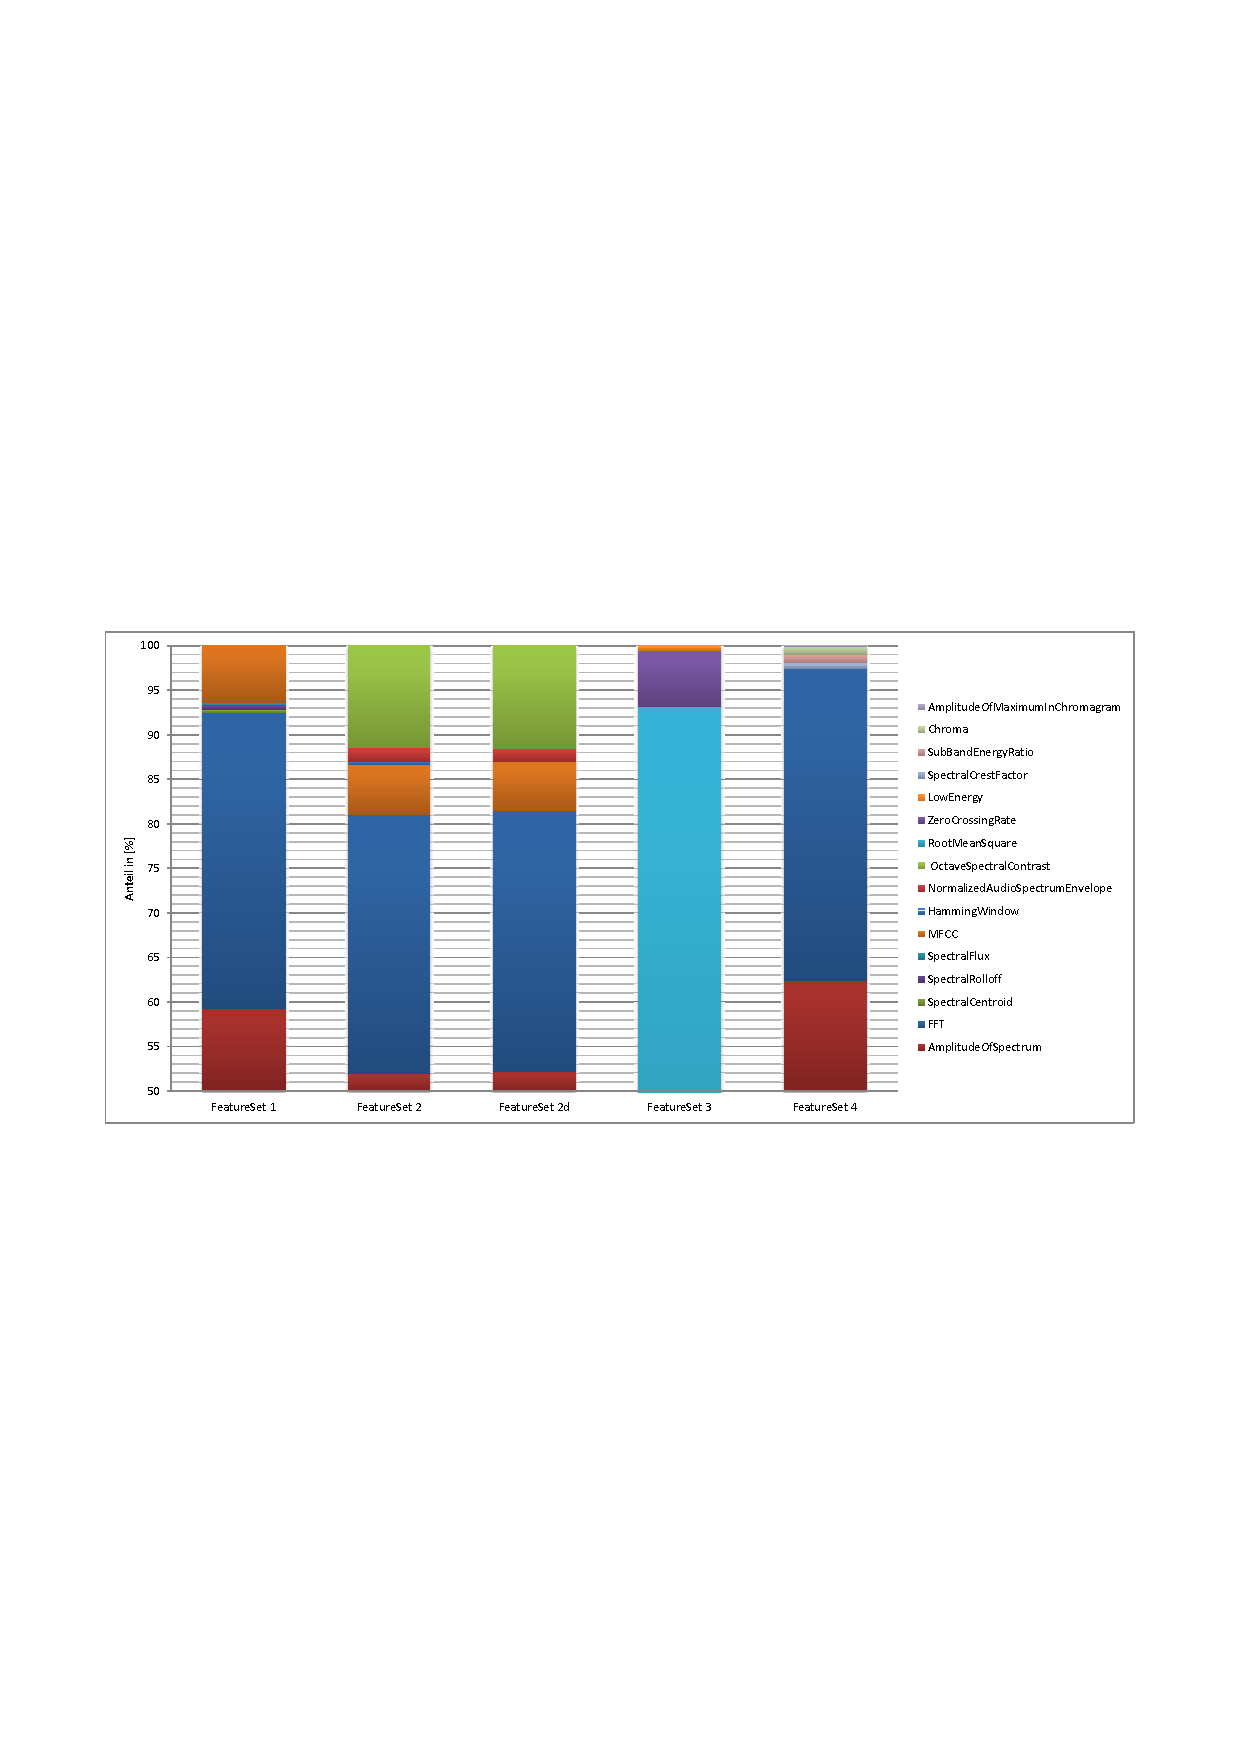
\includegraphics[width=1.00\textwidth]{../Pictures/ResultsExtraktionDSP.pdf}
	\caption{Laufzeitanteile der Features auf dem DSP}
	\label{fig:dsp}
\end{figure}

Es ist deutlich zu erkennen, dass in den FeatureSets 1 - 2d und 4 \textit{Amplitude of Spectrum} (\textbf{\ref{subsubsec:aos}}) und im FeatureSet 3 \textit{Root Mean Square} (\textbf{\ref{subsubsec:rms}}) die meiste Laufzeit in Anspruch nehmen, teilweise mit Anteilen weit �ber 50\%. Da beide Features eigentlich nur aus Summationen, Divisionen und der Bildung von Quadratwurzeln bestehen, die Bestandteil der Standartbibliotheken sind, scheint bei der Ausf�hrung von mathematischen Funktionen ein Bottleneck zu entstehen. Desweiteren ist zu sehen, dass auch bei der Umsetzung des Codes auf dem DSP ein weiterer Bottleneck bei der Ausf�hrung der FFT zu bestehen scheint, da auch diese mit ca. 30\% der Ausf�hrungszeit zu Buche schl�gt.

\section{Optimierung der Rechenfunktionen mit MATHLIB}\label{sec:mathlib}

\section{Optimierung der FFT mit DSPLIB}\label{sec:dsplib}

\section{Optimierung f�r den Compiler}\label{sec:compiler} 
\chapter{Evaluation}
\label{ch:results}
\rm
\chapter{Zusammenfassung und Ausblick}
\label{ch:sum}
\rm

\section{Zusammenfassung}\label{sec:summary}
Am Institut f�r Mikroelektronische System der Leibniz Universit�t Hannover werden in einem Projekt Algorithmen und Architekturen zur Konzeption Energie-effizienter Systeme zur Audio-Signalklassifikation untersucht. Hierbei wird der Entwurfsraum von Hardware-Architekturen zur Audio-Signalklassifikation insbedondere f�r mobile Endger�te exploriert.

Im Rahmen dieser Arbeit wurde eine heterogene Prozessorarchitektur der Firma Texas Instruments hinsichtlich der Laufzeiten und der Energie-Effizienz bei Anwendung der inhaltsbasierten Musikklassifikation untersucht. Hierbei wurde die rechenintensive Merkmalsextraktion von vier verschiedenen Musikklassififkationsmethoden f�r den ARM- und den DSP-Kern optimiert.

Nach der Optimierung wurden die Extraktionen auf dem Cortex A8 um Faktoren zwischen 2,5 (MCL3) und 22,5 (MCL4) beschleunigt. Die Beschleunigung der Extraktion auf dem C674x DSP geschah mit Faktoren zwischen 4,2 (MCL3) und 10,5 (MCL4)schneller als das portierte Referenz-Programm. Allgemeinen wird die Merkmalsextraktion auf dem DSP schneller ausgef�hrt als auf dem ARM Cortex A8.\\
Eine Musikklassifikation wird auf dem heterogenen System um das 1,2- bis 3,1-fache schneller verarbeitet als auf dem Cortex A8. Daraus folgt, dass unter dem Aspekt der Verarbeitungszeit das heterogene System das effektivere ist.\\
Wird die Energie-Effizienz betrachtet, so wurde festgestellt, dass ... um das ... effizienter ist als ... .\\

%\section{Ausblick}\label{sec:vista}
%
%Innerhalb dieser Arbeit wurde eine parallele Nutzung der beiden Prozessorkerne nicht betrachtet. Weiteres Forschungen sollten daher in Richtung des parallelen Einsatzes von ARM und DSP gehen. Hierbei sollte eine Verwendung des DSP zur Merkmalsextraktion angestrebt werden, bei der der DSP mehrere Musikst�cke verarbeitet und danach der ARM eine Prozessierung und Klassifikation dieser durchf�hrt, w�hrend weitere Musikst�cke auf dem DSP extrahiert werden.\\
%Des weiteren wurden nicht alle Optimierungsm�glichkeiten in vollem Ausma� ausgesch�pft, so dass auch in diese Richtung weitere Forschung geschehen sollte. Ans�tze f�r weiteres Optimierungspotenzial der Merkmalsextraktion auf ARM Cortex A8 und TI C674x DSP wurden in der Evaluation herausgestellt.

%bibtex Referenzen in bib datei
\bibliography{References/references}
\bibliographystyle{Macros/unsrtdin}
%\bibliographystyle{unsrt}
%Literaturverzeichnis ins Inhaltsverzeichnis
\addcontentsline{toc}{chapter}{Literaturverzeichnis}

\appendix %%Anhang
\renewcommand{\chaptermark}[1]{\markright{Appendix \thechapter\ \it #1}}
\renewcommand{\sectionmark}[1]{\markright{Appendix \thechapter\ \it #1}}
\renewcommand{\appendixname}{Anhang}
\renewcommand{\tablename}{Table}
\renewcommand{\figurename}{Figure}

\newpage
\thispagestyle{empty}
\mbox{}

\end{document}

